%%%%%%%%%%%%%%%%%%%%%%%%%%%%%%%%%%%%%%%%%%%%%%%%%%%%%%%%%%%%%%%%%%%%%%%%%%%
%%
%% Filename: 	spec.tex
%% {{{
%% Project:	ZipCPU -- a small, lightweight, RISC CPU soft core
%%
%% Purpose:	This LaTeX file contains all of the documentation/description
%%		currently provided with this ZipCPU soft core.  It supersedes
%%	any information about the instruction set or CPUs found elsewhere.
%%	It's not nearly as interesting, though, as the PDF file it creates, so
%%	I'd recommend reading that before diving into this file.  You should
%%	be able to find the PDF file in the git repository together with this
%%	PDF file and a copy of the GPL-3.0 license this file is distributed
%%	under.  If not, just type 'make' in the doc directory and it (should)
%%	build without a problem.
%%
%%
%% TODO:
%% - Discuss how we handle big vs little endian
%% - Update ZipCPU philosophy
%% - Update CPU Status register
%% - Rearrange how the ZipCPU peripherals are presented
%%	Should be in their own section, since not all peripherals are in the
%%	ZipSystem
%% - Rewrite the debugging port section
%% - Examples of using the ZipCPU's debugging port
%%	Resetting the CPU
%%	Halting the CPU
%%	Reading registers from the CPU
%%	Writing/updating registers within the CPU (only supports full word writ)
%%	Breakpoint handling
%%	Stepping through an instruction
%% How does the assembler generate compressed instructions?
%% The wrapper should leave cpu_break set if the CPU halts on a break, rather
%%	than trusting the user to read it on that particular clock cycle
%% The ZipDMA control bits are ... incorrect.
%%
%% Creator:	Dan Gisselquist
%%		Gisselquist Technology, LLC
%%
%%%%%%%%%%%%%%%%%%%%%%%%%%%%%%%%%%%%%%%%%%%%%%%%%%%%%%%%%%%%%%%%%%%%%%%%%%%
%% }}}
%% Copyright (C) 2015-2024, Gisselquist Technology, LLC
%% {{{
%% This program is free software (firmware): you can redistribute it and/or
%% modify it under the terms of the GNU General Public License as published
%% by the Free Software Foundation, either version 3 of the License, or (at
%% your option) any later version.
%%
%% This program is distributed in the hope that it will be useful, but WITHOUT
%% ANY WARRANTY; without even the implied warranty of MERCHANTIBILITY or
%% FITNESS FOR A PARTICULAR PURPOSE.  See the GNU General Public License
%% for more details.
%%
%% You should have received a copy of the GNU General Public License along
%% with this program.  (It's in the $(ROOT)/doc directory, run make with no
%% target there if the PDF file isn't present.)  If not, see
%% <http://www.gnu.org/licenses/> for a copy.
%% }}}
%% License:	GPL, v3, as defined and found on www.gnu.org,
%% {{{
%%		http://www.gnu.org/licenses/gpl.html
%%
%%
%%%%%%%%%%%%%%%%%%%%%%%%%%%%%%%%%%%%%%%%%%%%%%%%%%%%%%%%%%%%%%%%%%%%%%%%%%%
%
%
%
% From TI about DSPs vs FPGAs:
%	www.ti.com/general/docs/video/foldersGallery.tsp?bkg=gray
%	&gpn=35145&familyid=1622&keyMatch=DSP Breaktime Episode Three
%	&tisearch=Search-EN-Everything&DCMP=leadership
%	&HQS=ep-pro-dsp-leadership-problog-150518-v-en
%
%	FPGA's are annoyingly faster, cheaper, and not quite as power hungry
%	as they used to be.
%
%	Why would you choose DSPs over FPGAs?  If you care about size,
%	if you care about power, or happen to have a complicated algorithm
%	that just isn't simply doing the same thing over and over
%
%	For complex algorithms that change over time.  Each have their strengths
%	sometimes you can use both.
%
%	"No assembly required" -- TI tools all C programming, very GUI based
%	environment, very little optimization by hand ...
%
%
% The FPGA's Achille's heel: Reconfigurability.  It is very difficult, although
% I'm sure major vendors will tell you not impossible, to reconfigure an FPGA
% based upon the need to process time-sensitive data.  If you need one of two
% algorithms, both which will fit on the FPGA individually but not together,
% switching between them on the fly is next to impossible, whereas switching
% algorithm within a CPU is not difficult at all.  For example, imagine 
% receiving a packet and needing to apply one of two data algorithms on the
% packet before sending it back out, and needing to do so fast.  If both
% algorithms don't fit in memory, where does the packet go when you need to
% swap one algorithm out for the other?  And what is the cost of that "context"
% swap?
%
% }}}
\documentclass{gqtekspec}
%% {{{
\usepackage{import}
\usepackage{bytefield}	% Install via apt-get install texlive-science
% \graphicspath{{../gfx}}
\project{ZipCPU}
\title{Specification}
\author{Dan Gisselquist, Ph.D.}
\email{dgisselq (at) ieee.org}
\revision{Rev.~3.0}
\definecolor{webred}{rgb}{0.5,0,0}
\definecolor{webgreen}{rgb}{0,0.4,0}
\hypersetup{
	hypertexnames,
	pdfauthor={Dan Gisselquist},
	pdfsubject={ZipCPU},
	anchorcolor= black,
	colorlinks = true,
	linkcolor  = webred,
	citecolor  = webgreen
}
%% }}}
\begin{document}
\pagestyle{gqtekspecplain}
\titlepage
\begin{license}
%% {{{
Copyright (C) \theyear\today, Gisselquist Technology, LLC

This project is free software (firmware): you can redistribute it and/or
modify it under the terms of the GNU General Public License as published
by the Free Software Foundation, either version 3 of the License, or (at
your option) any later version.

This program is distributed in the hope that it will be useful, but WITHOUT
ANY WARRANTY; without even the implied warranty of MERCHANTIBILITY or
FITNESS FOR A PARTICULAR PURPOSE.  See the GNU General Public License
for more details.

You should have received a copy of the GNU General Public License along
with this program.  If not, see \hbox{$<$http://www.gnu.org/licenses/$>$} for
a copy.
\end{license}
%% }}}
\begin{revisionhistory}
%% {{{
% Revision History
3.01 & 6/26/2022 & Gisselquist & Removed the last remains of the (unused) cpudefs macro file\\\hline
3.0 & 6/18/2022 & Gisselquist & New ZipDMA, debug interface, multi-bus support and bus width independence\\\hline
2.01 & 10/19/2019 & Gisselquist & Fixed CIS OpCode Table\\\hline
2.0 & 1/18/2017 & Gisselquist & Switched from 32--bit to 8--bit bytes.\\\hline
1.1 & 11/28/2016 & Gisselquist & Moved the ZipSystem address to {\tt 0xff000000} base.\\\hline
1.0 & 11/4/2016 & Gisselquist & Major rewrite,
			includes compiler info\\\hline
0.91& 7/16/2016 & Gisselquist & Described three more CC bits\\\hline
0.9 & 4/20/2016 & Gisselquist & Modified ISA: LDIHI replaced with MPY,
	MPYU and MPYS replaced with MPYUHI, and MPYSHI respectively.  LOCK
	instruction now permits an intermediate ALU operation. \\\hline
0.8 & 1/28/2016 & Gisselquist & Reduced complexity early branching \\\hline
0.7 & 12/22/2015 & Gisselquist & New Instruction Set Architecture \\\hline
0.6 & 11/17/2015 & Gisselquist & Added graphics to illustrate pipeline discussion.\\\hline
0.5 & 9/29/2015 & Gisselquist & Added pipelined memory access discussion.\\\hline
0.4 & 9/19/2015 & Gisselquist & Added DMA controller, improved stall information, and self--assessment info.\\\hline
0.3 & 8/22/2015 & Gisselquist & First completed draft\\\hline
0.2 & 8/19/2015 & Gisselquist & Still Draft, more complete \\\hline
0.1 & 8/17/2015 & Gisselquist & Incomplete First Draft \\\hline
\end{revisionhistory}
%% }}}
% Table of Contents, named Contents
\tableofcontents
\listoffigures
\listoftables
\begin{preface}
%% {{{
Many people have asked me why I am building the ZipCPU. ARM processors are
cheap and effective and ASIC processors will always have a better performance
than an FPGA soft-core processor.  Xilinx makes and markets Microblaze, Altera
Nios, and both have better toolsets than the ZipCPU.  The RISC--V ISA is
now well known among soft-core circles.  So, why build a new processor?

% Reason #1: Because I can
The easiest, most obvious answer is the simple one: Because I can.

% Reason #2: Open source, and vendor independance
There's more to it though. There's a lot of things that I would like to do with
a processor, and I want to be able to do them in a vendor independent fashion.
%%
%% 1.
First and foremost, I would like to be able to both simulate this processor
and place it inside an FPGA.  Without paying royalties, gate level ARM
simulations are out of the question.
%%
%% 2.
I would also like to be able to generate Verilog code, both for the processor
and the system it sits within, that can run equivalently on both Xilinx,
Altera, and Lattice chips, and that can be easily ported from one
manufacturer's logic architecture to another.
%%
%% 3.
Even more, before purchasing a chip or a board, I would like to know that my
soft core works.  That means that I'd like to build a test bench to test
components with, and Verilator is my chosen simulation tool. This forces me to
use all Verilog, and it prevents me from using any proprietary cores. For this
reason, ARM, Microblaze and Nios are out of the question.

% Reason #3: Light weight
Why not OpenRISC? Because the ZipCPU has different goals.  OpenRISC is designed
to be a full featured CPU.  The ZipCPU was designed to be a simple, resource
friendly, CPU.  The result is that it is easy to get a ZipCPU program running
on bare hardware for a special purpose application--such as what FPGAs were
designed for, although getting a full featured operating system on the ZipCPU
remains one of my eventual goals.  Further, the OpenRISC ISA is very complex,
defining over 200~instructions (even though most of them have has never been
fully implemented \ldots).  The ZipCPU on the other hand has only a small
handful of instructions, and all but the Floating Point instructions have
already been fully implemented.

% Reason #4: Learning
My final reason is that I'm building the ZipCPU as a learning experience. The
ZipCPU has allowed me to learn a lot about how CPUs work on a very micro
level. For the first time, I am beginning to understand many of the Computer
Architecture lessons from years ago.  Even at its third version, the ZipCPU
has continued to teach me more advanced topics such as verification and
regression testing.

To summarize: Because I can, because it is open source, because it is light
weight, and as an exercise in learning. 

% Reason #5: Update
Since building the ZipCPU initially in 2015, I've continued to work with it and
update it for many of the reasons above.  Now, however, I have a couple of new
reasons for using the ZipCPU as well.  For example, the ZipCPU has now formed
the basis for many contracts and as a portion of the deliverables within those
contracts.  The ZipCPU has also been a focus for learning about Verilog
simulation environments, formal verification, and how various bus structures
work.  For example, starting with version~3.0, the ZipCPU now supports
both AXI4 and AXI4-lite interfaces.

% Reason #6: Unfunded
Finally, let me say that even though the ZipCPU project has been unfunded, the
work that I have placed into it has been paid back nicely.  While working on
the ZipCPU, I have learned how to build a back end for GCC.  I later received
a contract for building a special GCC work-around to (post build) ``fix'' a
RISC--V processor that had made it into silicon, but with some instructions
not working.  Also, the ZipCPU's instruction fetch routines have formed the
basis for a scatter gather DMA implementation, for a scripted SONAR
transmitter, and will likely form the basis in the near future for a small
(I2C+SPI) telemetry system.  These facts now witness to the truth of the
Proverb, ``In all labour there is profit: but the talk of the lips tendeth
only to penury.'' (Prov 14:23)
\end{preface}
%% }}}

\chapter{Introduction}
%% {{{
\pagenumbering{arabic}
\setcounter{page}{1}

The ZipCPU is a soft--core CPU.  It has been designed to be small in area,
with only a minimal instruction set.

The basic philosophy of the ZipCPU is driven from a desire to minimize
logic, while maintaining the ability to be a fully pipelined, 32--bit
CPU capable of running a modern operating system (sans MMU).  It should run
nicely in a small area, while maintaining compatibility with many FPGA
architectures.

You might think of the ZipCPU as a poor man's alternative to the larger
architectures prevalent today.
%% }}}
\chapter{Key Features}\label{chap:features}
%% {{{
Some of the Key Features of the ZipCPU are listed below:

\begin{itemize}
\item 32--bit Architecture: All registers are 32-bits, addresses are 32-bits,
		instructions are 32-bits wide, etc.

\item A RISC CPU.  There is no microcode for executing instructions.
	Where possible, all instructions have been designed to be completed
	in a single clock cycle.

\item A Load/Store architecture.  Only load and store instructions
	can access memory.

\item There are no I/O instructions.  Attached peripherals are memory
	mapped, and external to the CPU.

\item Big Endian

\item A compressed instruction subset provides some amount of instruction
	compression for the most commonly used instructions.

\item A Von-Neumann architecture.  Both instructions and data share a 
	common addressing space.

\item A pipelined architecture, having stages for {\bf Prefetch},
	{\bf Decode}, {\bf Read-Operand}, a combined stage containing
	the {\bf ALU}, {\bf Memory}, and {\bf Divide} units, and then the
	final {\bf Write-back} stage.  See Fig.~\ref{fig:cpu}
\begin{figure}\begin{center}
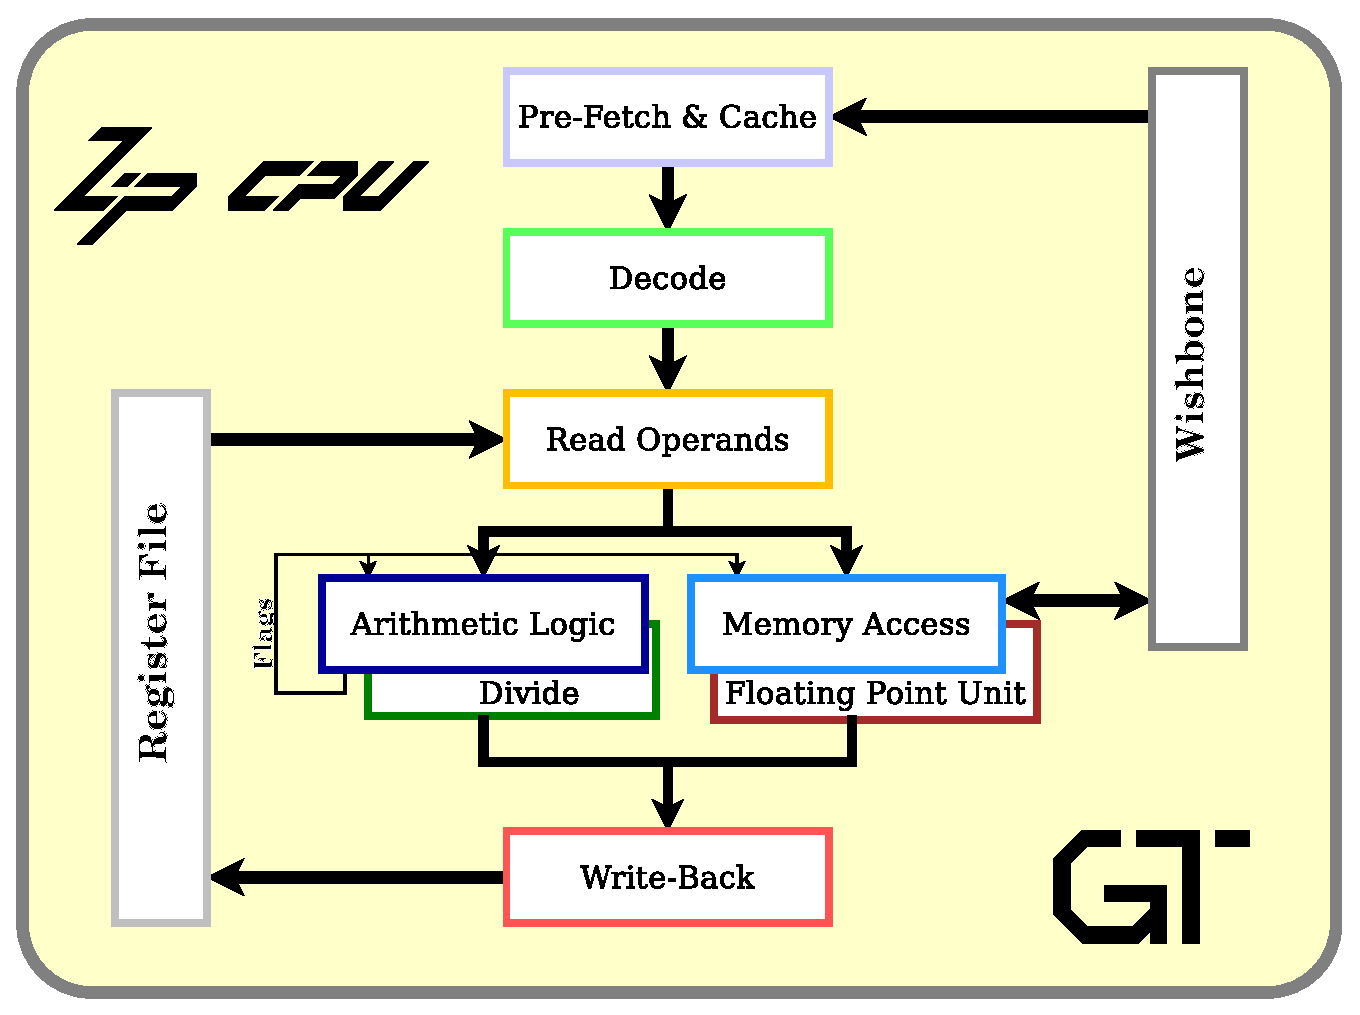
\includegraphics[width=3.5in]{../gfx/cpu.eps}
\caption{ZipCPU internal pipeline architecture}\label{fig:cpu}
\end{center}\end{figure}
	for a diagram of this structure.

\item Completely open source, licensed and released under the GPL v3.

\item The ZipCPU has several memory controllers.  These support Wishbone,
	AXI4--lite, and AXI4 bus structures, and may or may not provide a
	cache of user configurable size depending upon its configuration.

\item Bus-width agile.  The ZipCPU's memory controllers can handle any bus
	width of at least 32-bits.  Bus width configuration is parameterizable.

\item There is an (optional) external interface for debugging the CPU.  This
	allows an external debugger the ability to start, and stop the CPU,
	read and adjust its registers, or to step through any piece of software
	one instruction at a time.

\item The ZipCPU is also highly configurable, having optional support for
	clock gating, an external trace port, profiler, 
	multi-tasking, multiple multiply configurations, divide instruction
	support, early branching, and more.
\end{itemize}
%% }}}
\chapter{CPU Architecture}\label{chap:arch}
%% {{{
This chapter describes the general architecture of the ZipCPU.  It starts
with a description of the ZipCPU's instruction set.  From there, it moves
on to discuss how the ZipCPU handles interrupts, its pipeline, and then
the various memory controller options available to it.

\section{Instruction Set Architecture}\label{sec:isa}
%% {{{
The general form of (most) ZipCPU instructions is shown in
Tbl.~\ref{tbl:gen-insn}.
\begin{table}\begin{center}
\begin{tabular}{ll}
	{\tt OP.C}&{\tt Rb+\#Imm,Ra } \\
\end{tabular}%
\caption{The form of a generic ZipCPU instruction}\label{tbl:gen-insn}%
\end{center}\end{table}
In other words, the ZipCPU will apply some operation, {\tt OP}, to a register
plus an immediate, {\tt Rb+\#Imm}, and a second register, {\tt Ra},
while leaving the result in the same second register, {\tt Ra}.  If the
condition {\tt C} is present, the instruction will only complete if the
condition holds.

Unconditional ALU operations will set the condition code flags based upon
applying the operation to {\tt Rb+\#Imm} and {\tt Ra}.  Any overflow or
carry conditions due to adding {\tt Rb} and the immediate together will be
lost.

If the source register, {\tt Rb}, is the program counter register, {\tt PC},
than the immediate will be multiplied by four prior to adding it's value to
{\tt PC} to generate the {\tt Rb} value.

The next several sections will go into detail describing the register
set, instruction encoding, available operations, condition codes, and more.

\subsection{Operating Modes}
%% {{{
Before introducing the register set, it's important to know that
the ZipCPU supports two separate operating modes, a supervisor mode and a user
mode.  These modes are connected to interrupt handling: when operating in user
mode, interrupts are always enabled.\footnote{Interrupts may still be disabled
in the interrupt controller.}  When operating in supervisor mode,
interrupts are always disabled.

The CPU boots into supervisor mode.  The supervisor program can then cause
the CPU to switch to user mode by executing a special {\tt RTU} (return to
userspace) instruction.  When the CPU then encounters either an interrupt or
a fault, the CPU will return to supervisor mode {\em at the instruction where
it left off}.  This also means that the ZipCPU does not support any
interrupt vectors.
%% }}}
\subsection{Register Set}
%% {{{
The ZipCPU has two sets of sixteen 32-bit registers, one for supervisor mode
and the other for user mode.  These registers are shown in
Fig.~\ref{fig:regset}.
\begin{figure}\begin{center}
\begin{tabular}{|c|c|c|c|c|}
\multicolumn{2}{c}{Supervisor Register Set} &
	\multicolumn{1}{c}{} &
	\multicolumn{2}{c}{User Register Set} \\
\multicolumn{2}{c}{\#'s 0-15} & \multicolumn{1}{c}{} &
	\multicolumn{2}{c}{\#'s 16-31} \\\hline\hline
sR0(LR)	& sR8	&& uR0(LR) &	uR8	\\\cline{1-2}\cline{4-5}
sR1	& sR9	&& uR1	&	uR9	\\\cline{1-2}\cline{4-5}
sR2	& sR10	&& uR2	&	uR10	\\\cline{1-2}\cline{4-5}
sR3	& sR11	&& uR3	&	uR11	\\\cline{1-2}\cline{4-5}
sR4	& sR12(FP)&& uR4&	uR12(FP)\\\cline{1-2}\cline{4-5}
sR5	& sSP	&& uR5	&	uSP	\\\cline{1-2}\cline{4-5}
sR6	& sCC	&& uR6	&	uCC	\\\cline{1-2}\cline{4-5}
sR7	& sPC	&& uR7	&	uPC	\\\hline\hline
\multicolumn{2}{c}{Interrupts Disabled} &
	\multicolumn{1}{c}{} &
	\multicolumn{2}{c}{Interrupts Enabled} \\
\end{tabular}
\caption{ZipCPU Register File}\label{fig:regset}
\end{center}\end{figure}
Any switch from supervisor mode to user mode or back will also cause a sudden
shift from one register set to the other.  A special form of the {\tt MOV}
instruction exists to allow the supervisor access to user registers, but
otherwise the two register sets don't interact at all.  This effectively
means that the compiler knows nothing about the second register set.

Registers in either set may be referenced as {\tt R0} through {\tt R15}.
When running in supervisor mode, {\tt MOV} operand references to {\tt uR0}
through {\tt uR15} will be understood by the assembler as references to
user registers.  We'll discuss this further in subsection.~\ref{sec:isa-mov}.
In all other cases, any register reference refers to the currently active set.

Because the register sets are maintained when not in use, switching operating
modes has the consequence that the CPU maintains the appearance of continuing
where it left off when it last switched modes.  Similarly, the supervisor
may adjust the user register set to perform a task swap if and when desired.

Two registers in each set are special within the hardware.  These are the
Program Counter (PC, or R15), and the status register (CC, or R14).  When
using the compressed instruction set representation, offsets to R13 are
optimized within the instruction set to facilitate stack pointer accesses.
All other registers are identical in their hardware functionality.

By convention, the tool suite assigns a special meaning to three other
registers.  As mentioned above, the compiler reserves {\tt R13} for the
stack pointer.  This also has the mnemonic {\tt SP}.  By convention, {\tt R0}
is used to maintain the return address of a subroutine, sometimes called the
link register or {\tt LR}.  Finally, if the compiler requires a frame pointer,
then {\tt R12} (or {\tt FP}) is available to it for that purpose.
%% }}}
\subsection{The Status Register, CC}
%% {{{
As mentioned above, the status register (CC) is special.  The bit fields within
this register have special meaning, and so it really requires its own section.
These special bit-fields are shown in Fig.~\ref{tbl:cc-register},
\begin{table}\begin{center}
\begin{bitlist}
31\ldots 23 & R & Reserved\\\hline
22\ldots 16 & R/W & Reserved\\\hline
15 & W & Clear D-Cache command bit, always reads zero\\\hline
14 & W & Clear I-Cache command bit, always reads zero\\\hline
13 & R & Set if processing the first half of a compressed instruction\\\hline
12 & R & (Reserved for) Floating Point Exception\\\hline
11 & R & Division by Zero Exception\\\hline
10 & R & Bus-Error Flag\\\hline
9 & R & Trap Flag (or user interrupt).  Cleared on any return to user mode.\\\hline
8 & R & Illegal Instruction Flag\\\hline
7 & R/W & Break--Enable (sCC), or user break (uCC) encountered\\\hline
6 & R/W & Step\\\hline
5 & R/W & User mode / Global Interrupt Enable (GIE) bit\\\hline
4 & R/W & Sleep.  When GIE is also set, the CPU waits for an interrupt.\\\hline
3 & R/W & Overflow flag.  The last ALU operation produced an arithmetic
	overflow.\\\hline
2 & R/W & Negative.  The sign bit was set as a result of the last ALU
	instruction.\\\hline
1 & R/W & Carry.  The last ALU operation set the carry bit.\\\hline
0 & R/W & Zero.  The last ALU operation produced a zero.\\\hline
\end{bitlist}
\caption{Condition Code Register Bit Assignment}\label{tbl:cc-register}
\end{center}\end{table}
and occupy the lower sixteen bits of the status register.

Of the condition codes, the bottom four bits are the current flags from the
last ALU instruction that set flags.  These are:
		Zero (Z),
		Carry (C),
		Negative (N),
		and Overflow (V).
These flags maintain their usual definition from other CPUs that use them, for
all but the shift right instructions.  For example, if the result of the last
ALU operation is zero, the 'Z' flag will be set.  If the result of the last
ALU operation sets the most significant bit, then the 'N' flag will be set.
Carry is set according to unsigned operation overflow, and the overflow bit
is set according signed arithmetic overflow.

Local and arithmetic shift operations also use the carry bit to capture the
last bit shifted off the register.  This functionality isn't well supported
by the compiler, but can be used in assembly to implement extended shift
instructions.

We'll walk through the next many bits of the status register in order from
least significant to most significant.

\begin{enumerate}
	\setcounter{enumi}{3}
\item Bit 4 is the sleep bit.  When set, the CPU will enter into a sleep mode.
	The CPU will wake up and exit from sleep mode on any
	interrupt if interrupts are enabled.

	This means that this bit can be used to implement two functionalities.
	There's the {\tt WAIT} for interrupt instruction, whereby the CPU
	simply sleeps as discussed above in user mode.  This bit can also be
	used to {\tt HALT} the CPU should it ever be set while the CPU is in
	supervisor mode.  (The {\tt WAIT} instruction will place the CPU in
	user mode, independent of the mode it was in when executed.)

	If the {\tt OPT\_CLKGATE} parameter is set, the CPU will also turn off
	its clock once it finishes entering sleep mode.

\item Bit 5 is a global interrupt enable bit (GIE).
	When this bit is set, interrupts will be enabled, otherwise they are
	disabled.  When interrupts are disabled, the CPU will be in supervisor
	mode, otherwise it is in user mode.  This bit also forms the fifth bit
	of any register address, controlling which register set the CPU reads
	from by default.  Thus, to execute a context switch from supervisor
	mode to user mode, all one needs to do is to set this bit.  Then, on
	a subsequent interrupt or CPU exception, this bit will be automatically
	cleared and the CPU will return to supervisor mode.

	Logic within the CPU will prevent user mode software from setting
	the sleep register and clearing the GIE register at the same time,
	with clearing the GIE register taking precedence.  This keeps the
	user from halting the CPU, thus restricting the halt instruction to
	supervisor mode only.

	Whenever read, the supervisor CC register will always have this bit
	cleared, whereas the user CC register will always read this bit set.

\item Bit 6 is a step bit in the user's CC register, and zero in the
	supervisor's CC register.  It can only be read or set from supervisor
	mode.  When set, any switch to user mode will limit processing in user
	mode to a single instruction before returning to supervisor mode.

	There are two exceptions to this single instruction rule: a usermode
	program executing a compressed instruction will complete the full
	two-instruction sequence, and any usermode program executing a
	{\tt LOCK} instruction will complete an additional three instruction
	atomic sequence before concluding the step instruction.

	This functionality was added to allow one software program to debug
	a second program running in user space.

	While the CPU can also be stepped in supervisor mode, the supervisor's
	step bit is not used in that process.  Rather, that is accomplished
	via the CPU debug port.

\item Bit 7 is a break bit.

	In the user register set, this bit is a status bit that will be set if
	the user mode program encounters a {\tt BREAK} instruction.  It will
	automatically be cleared upon any release from interrupt.

	In the supervisor register set, this becomes the break enable control
	bit.  This bit determines if a usermode {\tt BREAK} instruction should
	generate an external break (break enabled), or just return processing
	to the supervisor mode.

	A break in supervisor mode will also cause an ``external break'',
	independent of the break enable bit.

	External breaks are handled by the CPU's wrapper.  If the CPU is set to
	{\tt START\_HALTED}, such breaks will halt the CPU.  Otherwise, they
	will cause the CPU to reboot.

	This functionality was added to enable a (potential) external debugger
	to set and manage software breakpoints.

\item Bit 8 is an illegal instruction bit.  When the CPU attempts to
	execute either a non-existent instruction, or an instruction from
	an address that produced a bus error when read, this bit will
	get set.  If set in user mode, the CPU will switch to supervisor mode.
	If an illegal instruction is encountered in supervisor mode,
	the CPU will issue an external break as described by the break
	handling section above.

\item Bit 9 is a trap bit.  This bit is shared between both user and supervisor
	{\tt CC} registers.  It may be set by a usermode process to request a
	switch to supervisor mode--a soft interrupt if you will.  It is
	then cleared upon any subsequent return to user space.

	This bit allows a supervisor mode process to determine, following any
	switch to supervisor mode, if the switch was caused by a user request.

\item Bit 10 is a bus error flag.  This bit will be set following any bus
	error return response to either a load or store instruction.

	If such a bus error is encountered in user mode, then this bit will be
	set in the user's CC register and the CPU will switch to supervisor
	mode.  It will be cleared by any subsequent return to user mode
	instruction.

	If the bus error is instead encountered in supervisor mode, then this
	bit will be set in the supervisor's CC register and the CPU will
	generate an external break.

	Bus errors encountered by the instruction fetch pipeline are returned
	as illegal instructions, and therefore will not affect this bit.

\item Bit 11 is a division by zero exception flag.  This operates
	in a fashion similar to the bus error flag.  If the user attempts
	to use the divide instruction with a zero denominator, the system
	will switch to supervisor mode and set this bit in the user CC
	register.  The bit is automatically cleared upon any return to user
	mode, although it can also be manually cleared by the supervisor.  In
	a similar fashion, if the supervisor attempts to execute a divide by
	zero, the CPU will issue an external break and set this division by
	zero exception flag in the supervisor's CC register for the debugger
	to inspect.  This bit will automatically be cleared upon any CPU
	reset, or it may be manually cleared by the external debugger writing
	to this register.

\item Bit 12 is reserved for a hardware accelerated floating point error.
	This will operate in a similar fashion to both the bus error and
	the division by zero flags, only it will be set upon a (yet to
	be determined) floating point error.

\item Bit 13 is the compressed instruction set phase register.  This
	bit will be set on the first instruction of any compressed instruction
	set pair.  It can be used to capture whether or not a CPU fault
	occurred following the first instruction in a compressed instruction
	set pair.  This is a status bit only.

	The CPU (currently) has no ability to restart an operation in the
	middle of a compressed instruction set pair.

\item Bit 14 is a clear instruction cache bit.  The supervisor may write a one
	to this bit in order to cause the CPU instruction cache to be cleared.
	The bit always reads as a zero.

	Writing to this bit from user mode has no effect.

\item Bit 15 is a clear data cache bit.  The supervisor may write a one
	to this bit in order to cause the CPU data cache to be cleared.
	The bit always reads as a zero.

	Writing to this bit from user space has no effect.
\end{enumerate}

The upper 16-bits of this register a reserved.
%% }}}
\subsection{Instruction Format}\label{sec:isa-fmt}
%% {{{
In general, ZipCPU instructions fit in one of the formats shown in
Fig.~\ref{fig:iset-format}.
\begin{figure}\begin{center}
\begin{bytefield}[endianness=big]{32}
\bitheader{0-31}\\
\begin{leftwordgroup}{Standard}\bitbox{1}{0}\bitbox[tlr]{4}{}
		\bitbox[lrt]{5}{OpCode}
		\bitbox[lrt]{3}{}
		\bitbox{1}{0}
		\bitbox{18}{18-bit Signed Immediate} \\
\bitbox{1}{0}\bitbox[lr]{4}{DR}
		\bitbox[lrb]{5}{}
		\bitbox[lr]{3}{Cnd}
		\bitbox{1}{1}
		\bitbox{4}{BR}
		\bitbox{14}{14-bit Signed Immediate}\end{leftwordgroup} \\
\begin{leftwordgroup}{MOV}\bitbox{1}{0}\bitbox[lr]{4}{}
		\bitbox[lrt]{5}{5'hd}
		\bitbox[lrb]{3}{}
		\bitbox{1}{A}
		\bitbox{4}{BR}
		\bitbox{1}{B}
		\bitbox{13}{13-bit Signed Immediate}\end{leftwordgroup} \\
\begin{leftwordgroup}{LDI}\bitbox{1}{0}\bitbox[lrb]{4}{}
		\bitbox{4}{4'hc}
		\bitbox{23}{23-bit Signed Immediate}\end{leftwordgroup} \\
\begin{leftwordgroup}{NOOP}\bitbox{1}{0}\bitbox{3}{3'h7}
		\bitbox{1}{}
		\bitbox{2}{11}
		\bitbox{3}{xxx}
		\bitbox{22}{Ignored}
		\end{leftwordgroup} \\
\end{bytefield}
\caption{Zip Instruction Set Format}\label{fig:iset-format}
\end{center}\end{figure}
The basic format is that some operation, defined by the OpCode, is applied
if a condition, Cnd, is true in order to produce a result which is placed in
the destination register (DR).  The destination register also forms the "A"
operand of any instruction.  The ``B'' operand is formed from either an
18--bit signed immediate, or a 14--bit signed immediate plus the value
contained within a second register.

There are a couple of exceptions to this general instruction model.  The
first is the {\tt MOV} instruction, which steals bits~13 and~18 to allow
supervisor access to user registers.  In supervisor mode, these are set to
one to reference user registers, zero otherwise.  They are ignored in user
mode.  The second exception is the load 23--bit signed immediate instruction
({\tt LDI}).  This instruction accepts no conditions and uses only a 4-bit
opcode.  The third exception is the {\tt NOOP} instruction group, encoding the
{\tt BREAK}, {\tt LOCK}, {\tt SIM}, and {\tt NOOP} instructions.  These
instructions ignore their register and immediate settings.  Further, the
immediate bits used by these opcodes are available for simulation or debug
facilities, but otherwise ignored by the CPU.  Finally, there is an (optional)
compressed instruction format that we'll cover later.
%% }}}
\subsection{Instruction OpCodes}\label{sec:isa-opcodes}
%% {{{
32 possible instructions can be generated from a 5--bit opcode field.
Tbl.~\ref{tbl:iset-opcodes}.
\begin{table}\begin{center}
\begin{tabular}{|l|l|l|l|c|} \hline \rowcolor[gray]{0.85}
OpCode & & A-Reg & Instruction &Sets CC \\\hline\hline
5'h00 & {\tt SUB} & \multicolumn{2}{l|}{Subtract} &   \\\cline{1-4}
5'h01 & {\tt AND} & \multicolumn{2}{l|}{Bitwise And} &   \\\cline{1-4}
5'h02 & {\tt ADD} & \multicolumn{2}{l|}{Add two numbers} &   \\\cline{1-4}
5'h03 & {\tt OR}  & \multicolumn{2}{l|}{Bitwise Or} & Y \\\cline{1-4}
5'h04 & {\tt XOR} & \multicolumn{2}{l|}{Bitwise Exclusive Or} &   \\\cline{1-4}
5'h05 & {\tt LSR} & \multicolumn{2}{l|}{Logical Shift Right} &   \\\cline{1-4}
5'h06 & {\tt LSL} & \multicolumn{2}{l|}{Logical Shift Left} &   \\\cline{1-4}
5'h07 & {\tt ASR} & \multicolumn{2}{l|}{Arithmetic Shift Right} &   \\\hline

5'h08 & {\tt BREV} & \multicolumn{2}{l|}{Bit Reverse B operand into result}&  \\\cline{1-4}
5'h09 & {\tt LDILO} & \multicolumn{2}{l|}{Load Immediate Low} & N\\\hline
5'h0a & {\tt MPYUHI} & \multicolumn{2}{l|}{Upper 32 of 64 bits from an unsigned 32x32 multiply} &  \\\cline{1-4}
5'h0b & {\tt MPYSHI} & \multicolumn{2}{l|}{Upper 32 of 64 bits from a signed 32x32 multiply} & Y \\\cline{1-4}
5'h0c & {\tt MPY} & \multicolumn{2}{l|}{Lower 32 of 64 bits from a 32x32 bit multiply} & \\\hline
5'h0d & {\tt MOV} & \multicolumn{2}{l|}{Move OpB into Ra} & N \\\hline
5'h0e & {\tt DIVU} & R0-R13 & Divide, unsigned & Y \\\cline{1-4}
5'h0f & {\tt DIVS} & R0-R13 & Divide, signed &  \\\hline\hline
%
5'h10 & {\tt CMP} & \multicolumn{2}{l|}{Compare (Ra-OpB) to zero} & Y \\\cline{1-4}
5'h11 & {\tt TST} & \multicolumn{2}{l|}{Test (AND w/o setting result)} &   \\\hline
5'h12 & {\tt LW} & \multicolumn{2}{l|}{Load a 32-bit word from memory (OpB) into Ra} & \\\cline{1-4}
5'h13 & {\tt SW} & \multicolumn{2}{l|}{Store a 32-bit word from Ra into memory at (OpB)} &  \\\cline{1-4}
5'h14 & {\tt LH} & \multicolumn{2}{l|}{Load 16-bits from memory (opB) into Ra, clear upper 16 bits} & N \\\cline{1-4}
5'h15 & {\tt SH} & \multicolumn{2}{l|}{Store the lower 16-bits of Ra into memory at (OpB)} &  \\\cline{1-4}
5'h16 & {\tt LB} & \multicolumn{2}{l|}{Load 8-bits from memory (OpB) into Ra, clear upper 24 bits} & \\\cline{1-4}
5'h17 & {\tt SB} & \multicolumn{2}{l|}{Store the lower 8-bits of Ra into memory at (OpB)} &  \\\hline\hline
5'h18/9 & {\tt LDI} & \multicolumn{2}{l|}{Load 23--bit signed immediate} & N \\\hline\hline
5'h1a & {\tt FPADD} & R0-R13 & (Reserved for) Floating point add &  \\\cline{1-4}
5'h1b & {\tt FPSUB} & R0-R13 & (Reserved for) Floating point subtract &   \\\cline{1-4}
5'h1c & {\tt FPMPY} & R0-R13 & (Reserved for) Floating point multiply & Y \\\cline{1-4}
5'h1d & {\tt FPDIV} & R0-R13 & (Reserved for) Floating point divide &   \\\cline{1-4}
5'h1e & {\tt FPI2F} & R0-R13 & (Reserved for) Convert integer to floating point &   \\\cline{1-4}
5'h1f & {\tt FPF2I} & R0-R13 & (Reserved for) Convert floating point to integer &   \\\hline\hline
5'h1c & {\tt BREAK} &None(15)& Debugger break point & \\\cline{1-4}
5'h1d & {\tt LOCK} &None(15)& Begin an atomic access sequence & N\\\cline{1-4}
5'h1e & {\tt SIM}  &None(15)& Simulation--only instruction &\\\cline{1-4}
5'h1f & {\tt NOOP} &None(15)&&\\\hline
\end{tabular}
\caption{ZipCPU OpCodes}\label{tbl:iset-opcodes}
\end{center}\end{table}
shows how these 32--values have been allocated to implement 29~instructions.
An additional six instruction opcodes are reserved for a (potential, future,
optional) single precision floating point accelerator.

%% }}}
\subsection{Conditional Instructions}\label{sec:isa-cond}
%% {{{
Most, although not quite all, instructions may be conditionally executed.  
The 23--bit load immediate instruction, together with the special instructions,
{\tt NOOP}, {\tt SIM}, {\tt BREAK}, and {\tt LOCK}, are the exceptions to this
rule.  All other instructions may be conditionally executed.

From the four condition code flags, eight conditions are defined, as shown in
Tbl.~\ref{tbl:conditions}.
\begin{table}\begin{center}
\begin{tabular}{l|l|l}
Code & Mnemonic & Condition \\\hline
3'h0 & None & Always execute the instruction \\
3'h1 & {\tt .Z} & Zero.  Only execute when `Z' is set \\
3'h2 & {\tt .LT}& Less than.  Only execute when `N' is set \\
3'h3 & {\tt .C} & Carry set (Also known as less-than unsigned) \\
3'h4 & {\tt .V} & Overflow.  Only execute when `V' is set\\
3'h5 & {\tt .NZ}& Not zero.  Only execute when `Z' is clear \\
3'h6 & {\tt .GE}& Greater than or equal.  Executes when `N' is clear\\
3'h7 & {\tt .NC}& Not carry (also known as greater-than or equal, unsigned) \\
\end{tabular}
\caption{Conditions for conditional operand execution}\label{tbl:conditions}
\end{center}\end{table}
There are no condition codes for either less than or equal, or for greater
than, whether signed or unsigned.  In a similar fashion, there is no condition
code for not V.  Ways of handling non--supported conditions are discussed
in Sec.~\ref{sec:in-mcond}.

With the exception of \hbox{\tt CMP} and \hbox{\tt TST} instructions,
conditionally executed instructions will not further adjust the
condition codes.  This allows conditional instruction sequences to be
strung together.  Conditional \hbox{\tt CMP} or \hbox{\tt TST} instructions
will adjust conditions whenever they are executed.  In this way, multiple
conditions may be evaluated without branches, creating a sort of logical
and--but only if all the conditions are the same.  For example, to do
something if \hbox{\tt R0} is one and \hbox{\tt R1} is two, one might
implement the assembly shown in Tbl.~\ref{tbl:dbl-condition}.
\begin{table}\begin{center}
\begin{tabular}{l}
	{\tt CMP 1,R0} \\
	{\em ; Condition codes are now set based upon R0-1} \\
	{\tt CMP.Z 2,R1} \\
	{\em ; If R0 $\neq$ 1, conditions are unchanged, {\tt Z} is still false.} \\
	{\em ; If R0 $=$ 1, conditions are now set based upon R1-2.} \\
	{\em ; Now some instruction could be done based upon the conjunction} \\
	{\em ; of both of these conditions.} \\
	{\em ; While we use the example of a {\tt SW}, it could easily be any
		other instruction.} \\
	{\tt SW.Z R0,(R2)} \\
\end{tabular}
\caption{An example of a double conditional}\label{tbl:dbl-condition}
\end{center}\end{table}
This ability to generate double conditions is used heavily by the compiler
when comparing 64-bit numbers together.

The real utility of conditionally executed instructions is that, unlike
conditional branches, conditionally executed instructions will not clear the
pipeline if they are not executed.
%% }}}
\subsection{Modifying Conditions}\label{sec:in-mcond}
%% {{{
A quick look at the list of conditions supported by the ZipCPU and listed
in Tbl.~\ref{tbl:conditions} reveals that the ZipCPU does not have a full set
of conditions.  Tbl.~\ref{tbl:creating-conditions}, therefore,
\begin{table}\begin{center}
\begin{tabular}{|l|l|l|}\hline
Unsupported condition & Modified & Name \\\hline\hline
\parbox[t]{1.5in}{\tt CMP Imm,Ry\\BLE label} % If Ry <= Rx -> Ry < Rx+1
	& \parbox[t]{1.5in}{\tt CMP 1+Imm,Ry\\BLT label}
	& Less-than or equal (signed, {\tt Z} or {\tt N} set)\\[4mm]\hline
\parbox[t]{1.5in}{\tt CMP Rx,Ry\\BLE label} % If Ry <= Rx -> Ry < Rx+1
	& \parbox[t]{1.5in}{\tt CMP Rx,Ry\\BLT label\\BZ label}
	& Less-than or equal (signed, {\tt Z} or {\tt N} set)\\[4mm]\hline\hline
\parbox[t]{1.5in}{\tt CMP Imm,Ry\\BGT label}	% if (Ry > Rx) -> Rx < Ry
	& \parbox[t]{1.5in}{\tt CMP 1+Imm,Ry\\BGE label}
	& Greater-than (immediate) \\[4mm]\hline
\parbox[t]{1.5in}{\tt CMP Rx,Ry\\BGT label}	% if (Ry > Rx) -> Rx < Ry
	& \parbox[t]{1.5in}{\tt CMP Ry,Rx\\BLT label}
	& Greater-than (register) \\[4mm]\hline\hline
\parbox[t]{1.5in}{\tt CMP Imm,Ry\\BLEU label}
	& \parbox[t]{1.5in}{\tt CMP 1+Imm,Ry\\BC label}
	& Less-than or equal, unsigned immediate \\[4mm]\hline
\parbox[t]{1.5in}{\tt CMP Rx,Ry\\BLEU label}
	& \parbox[t]{1.5in}{\tt CMP Ry,Rx\\BNC label}
	& Less-than or equal unsigned register\\[4mm]\hline\hline
\parbox[t]{1.5in}{\tt CMP Imm,Ry\\BGTU label}	% if (Ry > Rx) -> Rx < Ry
	& \parbox[t]{1.5in}{\tt CMP 1+Imm,Ry\\BNC label}
	& Greater-than unsigned (immediate)\\[4mm]\hline
\parbox[t]{1.5in}{\tt CMP Rx,Ry\\BGTU label}	% if (Ry > Rx) -> Rx < Ry
	& \parbox[t]{1.5in}{\tt CMP Ry,Rx\\BC label}
	& Greater-than unsigned \\[4mm]\hline
\end{tabular}
\caption{Modifying conditions}\label{tbl:creating-conditions}
\end{center}\end{table}
shows examples of how these unsupported conditions can be created simply by
adjusting the compare instruction, for no extra cost in clocks.
Care needs to be taken to ensure that adding one to any immediates, as shown
above, does not overflow the size of the immediate field.

Many of these alternate conditions are chosen automatically by the ZipCPU
compiler.
%% }}}
\subsection{Operand B}\label{sec:isa-opb}
%% {{{
Many instruction forms have a 19-bit source ``Operand B'', or OpB for short,
associated with them.  This ``Operand B'' is shown in
Fig.~\ref{fig:iset-format} as part of the standard instruction format.  For
all but the {\tt MOV} instruction, an Operand B is either equal to a register
plus a 14--bit signed immediate offset, or an 18--bit signed immediate offset
by itself.  This value is encoded as shown in Tbl.~\ref{tbl:opb}.
\begin{table}\begin{center}
\begin{bytefield}[endianness=big]{19}
\bitheader{0-18}  \\
\bitbox{1}{0}\bitbox{18}{18-bit Signed Immediate} \\
\bitbox{1}{1}\bitbox{4}{Reg}\bitbox{14}{14-bit Signed Immediate}
\end{bytefield}
\caption{Bit allocation for Operand B}\label{tbl:opb}
\end{center}\end{table}
This format represents a deviation from many other RISC architectures that use
{\tt R0} to represent zero, such as OpenRISC and RISC-V.  Here, instead, we use
a bit within the instruction to note whether or not an immediate is used.
The result is that ZipCPU instructions can encode larger immediates within
their instruction space.

In those cases where a fourteen or eighteen bit immediate doesn't make sense,
such as for {\tt LDILO}, the extra bits associated with the immediate are
simply ignored.  (This rule does not apply to the shift instructions,
{\tt ASR}, {\tt LSR}, and {\tt LSL}--which all use all of their immediate bits.)
%% }}}
\subsection{Address Modes}\label{sec:isa-addr}
%% {{{
Load and store instructions use the OpB field for their address, whether
source or destination.  As a result, the ZipCPU can support both register plus
immediate addressing, as well as a limited amount of immediate addressing.
%% }}}
\subsection{Move Operands}\label{sec:isa-mov}
%% {{{
The {\tt MOV} instruction is the exception to operand B encoding, with the
purpose of providing the supervisor access to user mode registers while in
supervisor mode.  The two bits, shown as {\tt A} and {\tt B} in
Fig.~\ref{fig:iset-format} above, are designed to contain the high order bit
of the 5--bit register index.  If the {\tt B} bit is a `1', the source operand
comes from the user register set.  If the {\tt A} bit is a `1', the
destination operand is in the user register set.  A zero bit indicates the
current register set.

This encoding has been chosen to keep the compiler simple.  For the most part,
the extra bits are quietly set to zero.  Special assembly instructions,
or particular compiler built--in instructions, can be used to get access to
these cross register set move instructions.

Further, the {\tt MOV} instruction lacks the full OpB capability to use a
register or a register plus immediate as a source, since a load immediate
instruction, {\tt LDI}, already exists.  As a result, all moves come from a
register plus a potential offset.

This also creates a situation where a {\tt MOV} instruction may be used
like a 3-operand {\tt ADD} instruction.  Because the {\tt MOV} instruction
doesn't affect the condition codes, the compiler may use this instruction
during address calculation.
%% }}}
\subsection{Multiply Operations}\label{sec:isa-mpy}
%% {{{
The ZipCPU supports three separate 32x32-bit multiply instructions: {\tt MPY},
{\tt MPYUHI}, and {\tt MPYSHI}.  The first of these produces the low 32-bits
of a 32x32-bit multiply result.  The second two produce the upper 32-bits.
{\tt MPYUHI} produces the upper 32-bits assuming the multiply was unsigned,
whereas {\tt MPYSHI} produces the same bits for signed multiplication.  Each
multiply instruction is independent of every other in execution, although
the compiler is likely to use them as though they were dependent.

In an effort to maintain a fast clock speed, all three of these multiplies
have been slowed down in logic.  Thus, depending upon the setting of
the {\tt OPT\_MULTIPLY} parameter, the multiply instructions
will either 1)~cause an ILLEGAL instruction error ({\tt OPT\_MULTIPLY=0}, or
no multiply support), or take {\tt OPT\_MULTIPLY} additional clock
cycles to complete.

Several multiplication implementations exist, as shown in
Tbl.~\ref{tbl:opt-multiply}.
\begin{table}\begin{center}
\begin{tabular}{c|p{5in}}
{\tt OPT\_MULTIPLY} & Implementation\\\hline\hline
0 & No multiply support \\\hline
1 & Single clock multiply.  This implementation neither registers
	the inputs to the multiplier, nor the output prior to the ALU
	output result.\\\hline
2 & Two clock multiply.  This implementation registers the inputs to the
	multiply unit, but the outputs are not registered prior to the
	ALU mux.\\\hline
3 & Three clock multiply.  This implementation registers the inputs to the
	multiply unit as well as the outputs immediately following the
	multiply and prior to the final ALU register.  This is the workhorse
	of most FPGA DSP implementations, although it does require a DSP
	or DSP combination capable of implementing a 32x32 multiply in a single
	clock cycle.\\\hline
4 & Four clock multiply.  This implementation splits the multiply into
	multiple sixteen bit multiplies in a FOIL (first, outer, inner, last)
	binomial multiplication fashion.  The first clock registers the
	inputs.  The second clock calculates all FOIL values, and the third
	clock adds the results together to form a full 64-bit multiply result.
	This method is appropriate for DSP implementations that can handle
	16x16 bit multiplies but cannot be combined to implement a 32x32 bit
	multiply.
	\\\hline
5+ & Slow multiply.  This implementation uses (roughly) 32-cycles to achieve
	a full multiply result.  This is the one implementation that does not
	use hardware multiply (DSP) support.\\\hline
\end{tabular}
\caption{Multiply implementation choices}\label{tbl:opt-multiply}%
\end{center}\end{table}
%% }}}
\subsection{Divide Unit}
%% {{{
The ZipCPU also has an optional divide unit which can be built alongside the
ALU.  This divide unit provides the ZipCPU with another two instructions that
cannot be executed in a single cycle: {\tt DIVS}, or signed divide, and
{\tt DIVU}, the unsigned divide.  These are both 32--bit divide instructions,
dividing one 32--bit number by another.  In this case, the Operand B field,
whether it be register or register plus immediate, constitutes the denominator,
whereas the numerator is given by the other register.

As with the multiply, the divide instructions are also multi--clock
instructions.  While the divide is running, the ALU, any memory loads, and the
floating point unit (if installed) will all be idle.  Once the divide completes,
other units may be activated.

Should the divisor be zero, the divide will result in a division by zero
exception.  Upon exception, the divide by zero bit will be set in the
appropriate CC~register.  In the case of a user mode divide by zero, this will
be cleared by any return to user mode command.  The supervisor bit may be
cleared either by either a reboot or by a write from the external debugger.
%% }}}
\subsection{Compressed Instructions}
%% {{{
The ZipCPU also supports a compressed instruction set (CIS), as outlined in
Fig.~\ref{fig:iset-cis},
\begin{figure}\begin{center}
\begin{bytefield}[endianness=big]{16}
\bitheader{0-15}\\
\bitbox[lrt]{1}{}\bitbox[lrt]{4}{}
		\bitbox[lrt]{3}{COp}
		\bitbox{1}{0}
		\bitbox{7}{Imm.} \\
\bitbox[lr]{1}{1}\bitbox[lr]{4}{DR}
		\bitbox[lrb]{3}{}
		\bitbox{1}{1}
		\bitbox{4}{BR}
		\bitbox{3}{Imm} \\
\bitbox[lr]{1}{}\bitbox[lr]{4}{}
		\bitbox{3}{\tt LDI}
		\bitbox{8}{8'b Imm} \\
\bitbox[lrb]{1}{}\bitbox[lrb]{4}{}
		\bitbox{3}{\tt MOV}
		\bitbox{1}{1}
		\bitbox{4}{BR}
		\bitbox{3}{Imm} \\
\end{bytefield}
\caption{ZipCPU Compressed Instruction Set (CIS) Format}\label{fig:iset-cis}
\end{center}\end{figure}
when enabled via {\tt OPT\_CIS}.
This compressed instruction set packs two instructions per word.  Words
must still be aligned, and jumping into the middle of a compressed instruction
is not (currently) allowed.  Interrupts, therefore, are disabled between the
two instructions.  Further, the CIS only permits the encoding of 8~of the
32~opcodes available in the ISA.  These eight compressed opcodes are listed
in Tbl.~\ref{tbl:iset-cisops}.
\begin{table}\begin{center}
\begin{tabular}{|l|l|l|} \hline \rowcolor[gray]{0.85}
COp & & Instruction \\\hline\hline
3'h0 & {\tt SUB} & Subtract   \\\hline
3'h1 & {\tt AND} & Bitwise And   \\\hline
3'h2 & {\tt ADD} & Add two numbers   \\\hline
3'h3 & {\tt CMP}  & Compare \\\hline
3'h4 & {\tt LW} & Load 32-bit word\\\hline
3'h5 & {\tt SW} & Store 32-bit word\\\hline
3'h6 & {\tt LDI} & Load immediate\\\hline
3'h7 & {\tt MOV} & Move\\\hline
\end{tabular}
\caption{CIS OpCodes}\label{tbl:iset-cisops}
\end{center}\end{table}

A final feature of the compressed instruction set has to do with load and
store instructions.  All CIS load and store instructions use the form
{\tt Rb+\#Imm}.  The instruction encoding that would otherwise be for
an {\tt \#Imm} alone has been made into a shorthand for using the stack pointer
as {\tt Rb} with an offset.  Hence the compressed instruction set allows loads
and stores to offsets of the Stack Pointer of -128~octets on up to~127 octets.
In practice, this gives the compressed load and store instructions, when
referencing the stack, thirty--two words that they can reference.

This compressed instruction set is somewhat similar to other architectures that
have a thumb instruction set, with the difference that the ZipCPU can intermix
regular and compressed instructions at will.  When using the CIS, instructions
are still issued one at a time, however interrupts are disabled between
instruction halves in order to prevent the CPU from stopping and then needing
to re-start mid-instruction.  Further, it is the silent job of the assembler
to generate CIS instructions in an opportunistic fashion--unless this feature
has been disabled on the command line.

The disassembler represents CIS instructions by placing a vertical bar
between the two components, while still leaving them on the same line.

Compressed instructions do not support conditional execution.
%% }}}
\subsection{BREAK, Bus LOCK, SIM, and NOOP Instructions}
%% {{{
Four instructions within the opcode list in Tbl.~\ref{tbl:iset-opcodes}, have
been reserved for special operations.  These are the {\tt BREAK}, bus
{\tt LOCK}, {\tt SIM}, and {\tt NOOP} instructions.  These are encoded
according to Fig.~\ref{fig:iset-noop}.
\begin{figure}\begin{center}
\begin{bytefield}[endianness=big]{32}
\bitheader{0-31}\\
\begin{leftwordgroup}{BREAK}
\bitbox[lrt]{1}{}\bitbox[lrt]{3}{}
		\bitbox{1}{}\bitbox[lrt]{3}{}\bitbox{2}{00}\bitbox{22}{Reserved for debugger}
		\end{leftwordgroup} \\
\begin{leftwordgroup}{LOCK}
\bitbox[lr]{1}{0}\bitbox[lr]{3}{3'h7}
		\bitbox{1}{}\bitbox[lr]{3}{111}\bitbox{2}{01}\bitbox{22}{Ignored}
		\end{leftwordgroup} \\
\begin{leftwordgroup}{SIM}
\bitbox[lr]{1}{}\bitbox[lr]{3}{}\bitbox{1}{}
	\bitbox[lr]{3}{}\bitbox{2}{10}\bitbox[lrt]{22}{Reserved for Simulator} 
		\end{leftwordgroup} \\
\begin{leftwordgroup}{NOOP}
\bitbox[lrb]{1}{}\bitbox[lrb]{3}{}\bitbox{1}{}
	\bitbox[lrb]{3}{}\bitbox{2}{11}\bitbox[lrb]{22}{} 
	\end{leftwordgroup} \\
\end{bytefield}
\caption{NOOP/Break/LOCK Instruction Format}\label{fig:iset-noop}
\end{center}\end{figure}

The {\tt BREAK} instruction is useful for creating a debug instruction that
will halt the CPU without executing.  If in user mode, depending upon the
setting of the break enable bit, it will either switch to supervisor mode or
halt the CPU--depending upon where the user wishes to do his debugging.  The
lower 22~bits of this instruction are reserved for the debugger's use.

The {\tt LOCK} instruction forms the basis of the ZipCPU's atomic operation
support.  The {\tt LOCK} instruction is the first instruction of a four
instruction sequence that executes with interrupts disabled.  This sequence is
typically characterized by a {\tt LOCK} instruction, followed by a load
instruction, an ALU operation, and then a store instruction.  Using this four
instruction sequence, the
ZipCPU can perfom atomic ALU operations such as adds, subtracts, bit-wise
OR, bit-wise AND, and exclusive OR operations.  It can also be used to
implement atomic exchanges, test and set instructions, or compare and swap
instructions.  Since interrupts are disabled during {\tt LOCK} instructions,
the sequence can also be used for a short series of instructions in user mode
that need to execute with interrupts disabled.

The {\tt SIM} and {\tt NOOP} instructions need a touch more explaining.
These instructions have one meaning when run in simulation, and a separate
meaning when run in hardware.  From the CPU's standpoint, the {\tt SIM}
instruction is designed to be an illegal instruction in hardware (i.e. when the
{\tt OPT\_SIM} parameter is clear), and a {\tt NOOP} instruction when executed
in simulation.  When executed in hardware, the lower 22--bits of these
instructions are ignored.

In simulation, however, those lower 22--bits often have a meaning specifying
a simulation only instructions.

Both {\tt SIM} and {\tt NOOP} instructions, though, contain 22--bits that can
be used by a simulator if present.  The encoding of these 22-bits is identical,
so that programs that run in a simulator may run on actual hardware as well
(using the {\tt NOOP} encoding), or they may complain that they were unintended
to run on actual hardware, such as if the {\tt SIM} encoding were used.
Particular encodings allow for exiting the simulation with a known exit
code, {\tt $x$EXIT}, dumping either one or all registers, {\tt $x$DUMP}, 
or simpling sending a character to the simulator's standard output stream,
{\tt $x$OUT}--where $x$ is either {\tt N} for the {\tt NOOP} version of the
instruction, or {\tt S} for the {\tt SIM} version of the opcode.

The various {\tt NOOP} and {\tt SIM} encodings are listed in
Fig.~\ref{fig:iset-simop}.
\begin{figure}\begin{center}
\begin{bytefield}[endianness=big]{32}
\bitheader{0-31}\\
\begin{leftwordgroup}{$x$EXIT}
	%% {{{
		\bitbox{1}{0}
		%% Destination register
		\bitbox{1}{1}
		\bitbox{1}{1}
		\bitbox{1}{1}
		\bitbox{1}{}
		%% Op-Code
		\bitbox{1}{1}
		\bitbox{1}{1}
		\bitbox{1}{1}
		\bitbox{1}{1}
		\bitbox{1}{S}
		%% 22-bits
		\bitbox{2}{}
		\bitbox{12}{12'h01}
		\bitbox{8}{Rsrvd}
		\end{leftwordgroup} \\
	%% }}}
\begin{leftwordgroup}{$x$DUMP}
	%% {{{
		\bitbox{1}{0}
		%% Destination register
		\bitbox{1}{1}
		\bitbox{1}{1}
		\bitbox{1}{1}
		\bitbox{1}{}
		%% Op-Code
		\bitbox{1}{1}
		\bitbox{1}{1}
		\bitbox{1}{1}
		\bitbox{1}{1}
		\bitbox{1}{S}
		%% 22-bits
		\bitbox{2}{}
		\bitbox{12}{12'h02}
		\bitbox{8}{8'hff}
		\end{leftwordgroup} \\
	%% }}}
\begin{leftwordgroup}{$x$DUMP Rx}
	%% {{{
		\bitbox{1}{0}
		%% Destination register
		\bitbox{1}{1}
		\bitbox{1}{1}
		\bitbox{1}{1}
		\bitbox{1}{}
		%% Op-Code
		\bitbox{1}{1}
		\bitbox{1}{1}
		\bitbox{1}{1}
		\bitbox{1}{1}
		\bitbox{1}{S}
		%% 22-bits
		\bitbox{2}{}
		\bitbox{12}{12'h002}
		\bitbox{4}{0}
		\bitbox{4}{Reg}
		\end{leftwordgroup} \\
	%% }}}
\begin{leftwordgroup}{$x$DUMP uRx}
	%% {{{
		\bitbox{1}{0}
		%% Destination register
		\bitbox{1}{1}
		\bitbox{1}{1}
		\bitbox{1}{1}
		\bitbox{1}{}
		%% Op-Code
		\bitbox{1}{1}
		\bitbox{1}{1}
		\bitbox{1}{1}
		\bitbox{1}{1}
		\bitbox{1}{S}
		%% 22-bits
		\bitbox{2}{}
		\bitbox{12}{12'h02}
		\bitbox{4}{1}
		\bitbox{4}{uReg}
		\end{leftwordgroup} \\
	%% }}}
\begin{leftwordgroup}{$x$OUT Rx}
	%% {{{
		\bitbox{1}{0}
		%% Destination register
		\bitbox{1}{1}
		\bitbox{1}{1}
		\bitbox{1}{1}
		\bitbox{1}{}
		%% Op-Code
		\bitbox{1}{1}
		\bitbox{1}{1}
		\bitbox{1}{1}
		\bitbox{1}{1}
		\bitbox{1}{S}
		%% 22-bits
		\bitbox{2}{}
		\bitbox{12}{12'h02}
		\bitbox{4}{2}
		\bitbox{4}{Reg}
		\end{leftwordgroup} \\
	%% }}}
\begin{leftwordgroup}{$x$OUT uRx}
	%% {{{
		\bitbox{1}{0}
		%% Destination register
		\bitbox{1}{1}
		\bitbox{1}{1}
		\bitbox{1}{1}
		\bitbox{1}{}
		%% Op-Code
		\bitbox{1}{1}
		\bitbox{1}{1}
		\bitbox{1}{1}
		\bitbox{1}{1}
		\bitbox{1}{S}
		%% 22-bits
		\bitbox{2}{}
		\bitbox{12}{12'h02}
		\bitbox{4}{3}
		\bitbox{4}{uReg}
		\end{leftwordgroup} \\
	%% }}}
\begin{leftwordgroup}{$x$OUT \#Imm}
	%% {{{
		\bitbox{1}{0}
		%% Destination register
		\bitbox{1}{1}
		\bitbox{1}{1}
		\bitbox{1}{1}
		\bitbox{1}{}
		%% Op-Code
		\bitbox{1}{1}
		\bitbox{1}{1}
		\bitbox{1}{1}
		\bitbox{1}{1}
		\bitbox{1}{S}
		%% 22-bits
		\bitbox{2}{}
		\bitbox{12}{12'h004}
		\bitbox{8}{Imm}
		\end{leftwordgroup} \\
	%% }}}
\end{bytefield}
\caption{NOOP/SIM Sub-Instruction Format}\label{fig:iset-simop}
\end{center}\end{figure}
%% }}}
\subsection{Floating Point}
%% {{{
Although the ZipCPU does not (yet) have a floating point unit, the current
instruction set reserves six opcodes for floating point operations.  It also
reserves a bit in the CC register for treating floating point exceptions like
divide by zero errors.

This should allow a 32--bit floating point accelerator to be included within
the CPU, and to allow some amount of native support for 32--bit floating point
operations.  64--bit floating point instructions will still either need to be
emulated in software, or else they will need an external floating point
peripheral.

Until this FPU is built and integrated, or even afterwards if the floating
point unit is not installed by option, floating point instructions will
trigger an illegal instruction exception, which may be trapped and then
implemented in software.
%% }}}
\subsection{Derived Instructions}
%% {{{
The ZipCPU supports many other common instructions by construction, although
not all of them are single cycle instructions.  Tables~\ref{tbl:derived-1},
\ref{tbl:derived-2}, \ref{tbl:derived-3} and~\ref{tbl:derived-4} show how
many of these other instructions may be implemented on the ZipCPU.  Many of
these instructions will have assembly equivalents, such as the branch
instructions, to facilitate working with the CPU.
\begin{table}\begin{center}
\begin{tabular}{p{1.0in}p{1.5in}p{3in}}\\\hline
Mapped & Actual  & Notes \\\hline
{\tt ABS Rx}
	& \parbox[t]{1.5in}{\tt TST -1,Rx\\NEG.LT Rx}
	& Absolute value instruction.  This depends upon the derived
	{\tt NEG} instruction below, and so this expands into three
	instructions total.\\\hline
\parbox[t]{1.4in}{\tt ADD Ra,Rx\\ADDC Rb,Ry}
	& \parbox[t]{1.5in}{\tt Add Ra,Rx\\ADD.C \$1,Ry\\Add Rb,Ry}
	& Add with carry.  This capability does not extend easily past 64~bits.
	\\\hline
\hbox{\tt BRA.$x$ +/-\$Addr}
	& \hbox{\tt ADD.$x$ \$Addr+PC,PC}
	& Branch or jump on condition $x$.  Works for 18--bit
		signed address offsets.\\\hline
\hbox{\tt BZ \$Addr}
	& \hbox{\tt Add.Z \$Addr+PC,PC}
	& Branch on zero.  Also known as branch on equals.\\\hline
\hbox{\tt BNZ \$Addr}
	& \hbox{\tt Add.NZ \$Addr+PC,PC}
	& Branch on not-zero.  Also known as branch on not-equals.\\\hline
\hbox{\tt BLT \$Addr}
	& \hbox{\tt Add.LT \$Addr+PC,PC}
	& Branch on less than.\\\hline
\hbox{\tt BGE \$Addr}
	& \hbox{\tt Add.GE \$Addr+PC,PC}
	& Branch on greater than or equal to.\\\hline
\hbox{\tt BC \$Addr}
	& \hbox{\tt Add.C \$Addr+PC,PC}
	& Branch on carry, also known as branch on less-than unsigned.\\\hline
\hbox{\tt BNC \$Addr}
	& \hbox{\tt Add.NC \$Addr+PC,PC}
	& Branch on not carry.\\\hline
\hbox{\tt BV \$Addr}
	& \hbox{\tt Add.V \$Addr+PC,PC}
	& Branch on overflow.\\\hline

% {\tt BRA.Cond +/-\$Addr}
% 	& \parbox[t]{1.5in}{\tt LDI \$Addr,Rx \\ ADD.cond Rx,PC}
% 	& Branch/jump on condition.  Works for 23 bit address offsets, but
% 	costs a register and an extra instruction.  With LDIHI and LDILO
% 	this can be made to work anywhere in the 32-bit address space, but yet
% 	cost an additional instruction still. \\\hline
% {\tt BNC PC+\$Addr}
%	& \parbox[t]{1.5in}{\tt Test \$Carry,CC \\ ADD.Z PC+\$Addr,PC}
%	& Example of a branch on an unsupported
%		condition, in this case a branch on not carry \\\hline
{\tt BUSY } & {\tt ADD \$-1,PC} & Execute an infinite loop.\\
% {\tt CLRF Rx }	%% Has no assembler support
%	& {\tt XOR Rx,Rx}
%	& Clear Rx, while also setting the flags appropriately.\\\hline
{\tt CLR Rx}
	& {\tt LDI \$0,Rx}
	& Clears Rx, leaving the flags untouched.  This instruction can be
		compressed, but cannot be conditional. \\\hline
{\tt CLR.NZ Rx }
	& {\tt BREV.NZ \$0,Rx}
	& Clears Rx, leaving the flags untouched.  This instruction can be
		executed conditionally. The assembler will quietly choose
		between {\tt LDI} and {\tt BREV} depending upon the existence
		of the condition.\\\hline
{\tt HALT }
	& {\tt Or \$SLEEP,CC}
	& This only works when issued in interrupt/supervisor mode.  In user
	mode this is simply a wait until interrupt instruction.  \\\hline
\hbox{\tt JMP R6+\$Offset}
	& {\tt MOV \$Offset(R6),PC}
	& Only works for 15--bit aligned offsets.  Other offsets may require
		adding the offset first to R6 before jumping.\\\hline
\end{tabular}
\caption{Derived Instructions}\label{tbl:derived-1}
\end{center}\end{table}
\begin{table}\begin{center}
\begin{tabular}{p{1.1in}p{1.8in}p{3in}}\\\hline
Mapped & Actual  & Notes \\\hline
{\tt LJMP \$Addr}
	& \parbox[t]{1.5in}{\tt LW (PC),PC \\ {\em Address }}
	& Although this only works for an unconditional jump, and it only
	makes sense in an environment with a unified instruction and data
	address space, this instruction combination makes for a nice
	combination that can be adjusted by a linker at a later time.\\\hline
{\tt LJMP.$x$ \$Addr}
	& \parbox[t]{1.5in}{\tt LW.$x$ 4(PC),PC \\ ADD 4,PC \\ {\em Address }}
	& Implements a conditional long jump.\\\hline
{\tt LJSR \$Addr  }
	& \parbox[t]{1.5in}{\tt MOV \$8+PC,R0 \\ LW (PC),PC \\ {\em Address}}
	& Long jump-to-subroutine.  This is similar to the LJMP instruction,
	save that it stores the return address in {\tt R0}.
	\\\hline
{\tt JSR PC+\$Offset  }
	& \parbox[t]{1.5in}{\tt MOV \$4+PC,R0 \\ ADD \$Offset,PC}
	& This is similar to the jump and link instructions from other
	architectures, save only that it requires a specific link
	instruction, seen here as the {\tt MOV} instruction on the
	left.\\\hline
{\tt LDI \$val,Rx }
	& \parbox[t]{1.8in}{\tt BREV REV($val$)\&0x0ffff,Rx \\
			LDILO ($val$\&0x0ffff),Rx}
	& \parbox[t]{3.0in}{Since there's not enough instruction
		space to load a complete immediate value into any register,
		fully loading a register with a 32-bit value requires two
		cycles.  The {\tt LDILO} (load immediate low) instruction
		has been created to facilitate this together with {\tt BREV}.
		\\
	This is also the appropriate means for setting a register value
	to an arbitrary 32--bit value in a post--assembly link
	operation.}\\\hline
% \parbox[t]{1.5in}{\tt LSL \$1,Rx\\ LSLC \$1,Ry}
%	& \parbox[t]{1.5in}{\tt LSL \$1,Ry \\
%	LSL \$1,Rx \\
%	OR.C \$1,Ry}
%	& Logical shift left with carry.  Note that the
%	instruction order is now backwards, to keep the conditions valid.
%	That is, LSL sets the carry flag, so if we did this the other way
%	with Rx before Ry, then the condition flag wouldn't have been right
%	for an {\tt OR} correction at the end. \\\hline
% \parbox[t]{1.5in}{\tt LSR \$1,Rx \\ LSRC \$1,Ry}
%	& \parbox[t]{1.5in}{\tt BREV $1,Rz\\
%	LSR \$1,Ry \\
%	LSR \$1,Rx \\
%	OR.C Rz,Ry}
%	& Logical shift right with carry.  Again, notice the required backwards
%	ordering.\\\hline
{\tt NEG Rx} & \parbox[t]{1.5in}{\tt XOR \$-1,Rx \\ ADD \$1,Rx} & Negates Rx\\\hline
{\tt NEG.C Rx} & \parbox[t]{1.5in}{\tt MOV.C \$-1+Rx,Rx\\XOR.C \$-1,Rx}
	& Conditionally negates Rx\\\hline
{\tt NOT Rx } & {\tt XOR \$-1,Rx } & One's complement\\\hline
\end{tabular}
\caption{Derived Instructions, continued}\label{tbl:derived-2}
\end{center}\end{table}
\begin{table}\begin{center}
\begin{tabular}{p{1.0in}p{1.5in}p{3.2in}}\\\hline
{\tt POP Rx }
	& \parbox[t]{1.5in}{\tt LW \$(SP),Rx \\ ADD \$4,SP}
	& The compiler avoids the need for this instruction and the similar
	{\tt PUSH} instruction when setting up the stack by coalescing all
	the stack address modifications into a single instruction at the
	beginning of any stack frame.\\\hline
{\tt PUSH Rx}
	& \parbox[t]{1.5in}{\hbox{\tt SUB \$4,SP} 
	\hbox{\tt SW Rx,\$(SP)}}
	& Note that for pipelined operation, it helps to coalesce all the
	{\tt SUB}'s into one command, and place the {\tt SW}'s right
	after each other.
	\\\hline
% {\tt PUSH Rx-Ry}
%	& \parbox[t]{1.5in}{\tt SUB \$$4n$,SP \\
%	SW Rx,\$(SP)
%	\ldots \\
%	SW Ry,\$$4\left(n-1\right)$(SP)}
%	& Multiple pushes at once only need the single subtract from the
%	stack pointer.  This derived instruction is analogous to a similar one
%	on the Motorola 68k architecture, although the Zip Assembler
%	does not support the combined instruction.  This instruction
%	also supports pipelined memory access.\\\hline
% {\tt RESET}
%	& \parbox[t]{1in}{
%		\tt LDI~0xff000000,R2\\
%		LDI 1,R1\\
%		\hbox{SW R1,\$watchdog(R2)}\\BUSY}
%	& This depends upon the existence of a watchdog peripheral, and the
%	peripheral base address being preloaded into {\tt R12}.  The BUSY
%	instructions are required because the CPU will continue until the
%	{\tt SW} has completed.
%
%	Another opportunity might be to jump to the reset address from within
%	supervisor mode.\\\hline
{\tt RET} & {\tt MOV R0,PC}
	& This depends upon the return address either remaining in {\tt R0}
	from a prior {\tt JSR} instruction, or otherwise it needs to be
	restored prior to the return call.  \\\hline
{\tt SEXB Rx }
	& \parbox[t]{1.5in}{\tt LSL 24,Rx \\ ASR 24,Rx}
	& Signed extend an 8--bit value into a full word.\\\hline
{\tt SEXH Rx }	
	& \parbox[t]{1.5in}{\tt LSL 16,Rx \\ ASR 16,Rx}
	& Sign extend a 16--bit value into a full word.\\\hline
% {\tt STEPLSR Rr,Rt}
%	& \parbox[t]{1.5in}{\tt LSR \$1,Rr \\ XOR.C Rt,Rr}
%	& Step a Galois implementation of a Linear Feedback Shift Register, Rr,
%		using taps Rt \\\hline
{\tt STEP}
	& \parbox[t]{1.5in}{\tt OR \$Step|\$GIE,CC}
	& Steps a user mode process by one instruction\\\hline
{\tt SUBR Rx,Ry }
	% & \parbox[t]{1.5in}{\tt SUB 1+Rx,Ry\\ XOR -1,Ry} 
	& \parbox[t]{1.5in}{\tt XOR -1,Ry\\ADD 1+Rx,Ry} 
	& Ry is set to Rx-Ry, rather than the normal subtract which
	sets Ry to Ry-Rx. \\\hline
\parbox[t]{1.4in}{\tt SUB Ra,Rx\\SUBC Rb,Ry}
	& \parbox[t]{1.5in}{\tt SUB Ra,Rx\\SUB.C \$1,Ry\\SUB Rb,Ry}
	& Subtract with carry.  Note that the overflow flag may not be
	set correctly after this operation.\\\hline
% {\tt SWAP Rx,Ry }
%	& \parbox[t]{1.5in}{\tt XOR Ry,Rx \\ XOR Rx,Ry \\ XOR Ry,Rx} 
%	& While no extra registers are needed, this example
%	does take 3-clocks. \\\hline
{\tt TRAP \#X}
	& \parbox[t]{1.5in}{\tt LDI \$x,R1 \\ AND \textasciitilde\$GIE,CC }
	& This works because whenever a user lowers the \$GIE flag, it sets
	a TRAP bit within the uCC register.  Therefore, upon entering the 
	supervisor state, the CPU only need check this bit to know that it
	got there via a TRAP.  The trap could be made conditional by making
	the LDI and the AND conditional.  In that case, the assembler would
	quietly turn the LDI instruction into a {\tt BREV}/{\tt LDILO} pair,
	but the effect would be the same. \\\hline
{\tt TS Rx,Ry,(Rz)}
	& \hbox{\tt LDI 1,Rx}
		\hbox{\tt LOCK}
		\hbox{\tt LB (Rz),Ry}
		\hbox{\tt TEST Ry}
		\hbox{\tt SB.Z Rx,(Rz)}
	& A test and set instruction.  The {\tt LOCK} instruction insures
	that the next three instructions lock the bus between the instructions,
	so no one else can use it.  Thus guarantees that the operation is
	atomic.
	\\\hline
%
%
\end{tabular}
\caption{Derived Instructions, continued}\label{tbl:derived-3}
\end{center}\end{table}
\begin{table}\begin{center}
\begin{tabular}{p{1.0in}p{1.5in}p{3in}}\\\hline
{\tt TST Rx}
	& {\tt TST \$-1,Rx}
	& Set the condition codes based upon Rx without changing Rx.
	Equivalent to a CMP \$0,Rx.\\\hline
{\tt WAIT}
	& {\tt Or \$GIE | \$SLEEP,CC}
	& Wait until the next interrupt, then jump to supervisor/interrupt
	mode.
\end{tabular}
\caption{Derived Instructions, continued}\label{tbl:derived-4}
\end{center}\end{table}
%% }}}
%% }}}

\section{Interrupt Handling}
%% {{{
The ZipCPU does not maintain any interrupt vector tables.  If an interrupt
takes place, the CPU simply switches to from user to supervisor (interrupt)
mode.  Since getting to user mode in the first place required a return to
userspace instruction, {\tt RTU}, once the interrupt takes place the 
supervisor just simply starts executing code immediately after that
{\tt RTU} instruction.

Since the CPU may return from userspace after either an interrupt (hardware
generated), a trap (software generated), or an exception (a fault of some
type), it is up to the supervisor code that handles the transition to
determine which of the three has taken place.
%% }}}

\iffalse
\section{Pipeline Operation}	%% Do I still need this section?
%% FIXME
%% This section only applies to pipeline mode, and then only with *some*
%% prefetches.  It will be out of date the moment the MMU is added.
%% {{{
As mentioned in the introduction, and highlighted in Fig.~\ref{fig:cpu},
the ZipCPU supports a five stage pipeline.
\begin{enumerate}
\item {\bf Prefetch}: Reads instructions from memory.  If the CPU has been 
	configured with a cache, the cache has been integrated into the
	prefetch.  Stalls are also created here if the instruction isn't
	in the prefetch cache.

\item {\bf Decode}: Decodes an instruction into it's OpCode, register(s)
	addresses to be read, condition code, and immediate offset.  This
	stage also determines whether the flags will be read or set, whether
	registers will be read (and hence the pipeline may need to stall), or
	whether the result will be written back.  In many ways, simplifying
	the CPU has meant simplifying this particular pipeline stage and hence
	the instruction set architecture that it implements.

	This stage is also responsible for both normal and CIS decoding.
	Hence, following this stage, little information remains regarding
	whether or not the CPU was executing a CIS instruction.

\item {\bf Read Operands}: Read from the register file and applies any
	immediate values to the result.  There is no means of detecting or
	flagging arithmetic overflow or carry when adding the immediate to the
	operand.  This stage will stall if any source operand is pending
	and the immediate value is non--zero.

\item At this point, the processing flow splits into one of four tracks: An
	{\bf ALU} track which will accomplish a simple instruction, the
	{\bf MemOps} stage which handles load and store instructions, the
	{\bf divide} unit, and (eventually) the {\bf floating point} unit.
	\begin{itemize}
	\item Loads will stall non-load instructions in the read operands stage
		until the entire memory operation is complete, lest a register
		be read from the register file only to be updated unseen by the
		load.
	\item Condition codes are set upon completion of the ALU, divide,
		or FPU stage.  (Memory operations do not set conditions.)
	\item Issuing a non--pipelined memory instruction to the memory unit
		while the memory unit is busy will stall the entire pipeline
		until the memory unit is idle and ready to accept another
		instruction.
	\end{itemize}
\item {\bf Write-Back}: Conditionally writes the result of the instruction to
	the register file, applying the condition and any special CC logic.
	This routine is quad-entrant: either the ALU, the memory, the divide,
	or the FPU may commit a result.

	This is also the stage where any special condition code logic takes
	place such as controlling the {\tt SLEEP} or {\tt GIE} bits.
\end{enumerate}

The ZipCPU does not support out of order execution.  Therefore, if the memory
unit stalls, every other instruction stalls.  The same is true for divide or
floating point instructions--all other instructions will stall while waiting
for these to complete.  Memory stores, however, may take place concurrently
with non--memory operations, although memory reads (loads) cannot.

% \subsection{Instruction Cache}
% \subsection{Data Cache}

\subsection{Pipeline Stalls}
The processing pipeline can and will stall for a variety of reasons.  Some of
these are obvious, some less so.  Some of the reasons for pipeline stalls are
listed below:
\begin{itemize}
\item When the prefetch cache is exhausted

	This reason should be obvious.  If the prefetch cache doesn't yet have
	the instruction available, then a bubble must enter the pipeline on
	each clock cycle until an instruction can be made ready.

\item While waiting for the pipeline to load following any taken branch, jump,
	return from interrupt or switch to interrupt context (4 stall cycles,
	minimum)

Fig.~\ref{fig:bcstalls}
\begin{figure}\begin{center}
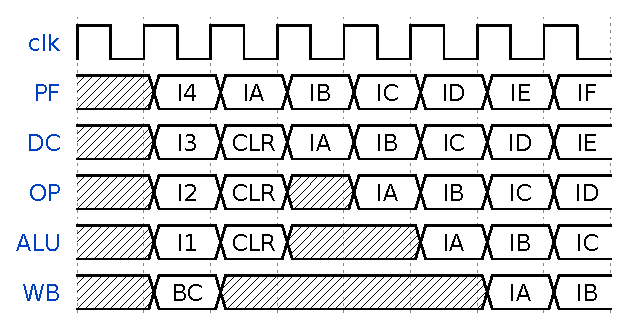
\includegraphics[width=3.5in]{../gfx/bc.eps}
\caption{A conditional branch generates 4 stall cycles}\label{fig:bcstalls}
\end{center}\end{figure}
illustrates the situation for a conditional branch.  In this case, the branch
instruction, {\tt BC}, is nominally followed by instructions {\tt I1} and so
forth.  However, since the branch is taken, the next instruction must be
{\tt IA}.  Therefore, the pipeline needs to be cleared and reloaded.  Given
that there are five stages to the pipeline, that accounts for the four stalls.

When the {\tt OPT\_EARLY\_BRANCHING} parameter is enabled, then the decode
stage will handle {\tt ADD \$X,PC}, and {\tt LW (PC),PC} in order to detect
and generate branches earlier in the pipeline.  These instructions, when not
conditioned on the flags, can execute with only a single stall cycle (two for
the {\tt LW (PC),PC} instruction), as shown in Fig.~\ref{fig:branch}.
\begin{figure}\begin{center}
\includegraphics[width=4in]{../gfx/bra.eps} %0.4in per clock
\caption{An expedited branch costs a single stall cycle}\label{fig:branch}
\end{center}\end{figure}
In this example, {\tt BR} is a branch always taken, {\tt I1} is the instruction
following the branch in memory, while {\tt IA} is the first instruction at the
branch address.  ({\tt CLR} denotes a clear--pipeline operation, and does
not represent any instruction.)

\item When reading from a prior register while also adding an immediate offset
\begin{enumerate}
\item\ {\tt OPCODE ?,RA}
\item\ {\em (stall)}
\item\ {\tt OPCODE I+RA,RB}
\end{enumerate}

	Since the addition of the immediate register within OpB decoding gets
	applied during the read operand stage so that it can be nicely settled
	before the ALU, any instruction that will write back an operand must
	be separated from the opcode that will read and apply an immediate
	offset by one instruction.  The good news is that this stall can
	easily be mitigated by proper scheduling.  That is, any instruction
	that does not add an immediate to {\tt RA} may be scheduled into the
	stall slot.

	This is also the reason why, when setting up a stack frame, the top
	of the stack frame is used first: it eliminates this stall
	cycle.\footnote{This only applies if there is no local memory to
	allocate on the stack as well.}  Hence, to save registers at the top
	of a procedure, one would write:
\begin{enumerate}
\item\ {\tt SUB 16,SP}
\item\ {\tt SW R1,(SP)}
\item\ {\tt SW R2,4(SP)}
\end{enumerate}
	Had {\tt R1} instead been stored at {\tt 4(SP)} as the top of the stack,
	there would've been an extra stall in setting up the stack frame.

\item When reading from the CC register after setting the flags
\begin{enumerate}
\item\ {\tt ALUOP RB,RA} {\em ; Ex: a compare opcode}
\item\ {\em (stall)}
\item\ {\tt TST sys.ccv,CC}
\item\ {\tt BZ somewhere}
\end{enumerate}

	The reason for this stall is simply performance: many of the flags are
	determined via combinatorial logic {\em during} the writeback cycle.
	Trying to then place these into the input for one of the operands for an
	ALU instruction during the same cycle
	created a time delay loop that would no longer execute in a single
	100~MHz clock cycle.  (The time delay of the multiply within the ALU
	wasn't helping either \ldots). 

	This stall may be eliminated via proper scheduling, such as by placing
	an instruction that does not set flags in between the ALU operation
	and the instruction that references the CC register.  For example,
	{\tt MOV \$addr+PC,uPC} followed by an {\tt RTU} ({\tt OR \$GIE,CC})
	instruction will not incur this stall, whereas an
	{\tt OR \$BREAKEN,CC} followed by an {\tt OR \$STEP,CC} will incur the
	stall, while a {\tt LDI \$BREAKEN|\$STEP,CC} will not since it doesn't
	read the condition codes before executing.

\item When waiting for a memory read operation to complete
\begin{enumerate}
\item\ {\tt LW address,RA}
\item\ {\em (bus dependent number of stalls)}
\item\ {\tt OPCODE I+RA,RB}
\end{enumerate}

	Remember, the ZipCPU does not support out of order execution.
	Therefore, anytime the memory unit becomes busy both the memory
	unit and the ALU must stall until the memory unit is cleared.  This
	is illustrated in Fig.~\ref{fig:memrd},
\begin{figure}\begin{center}
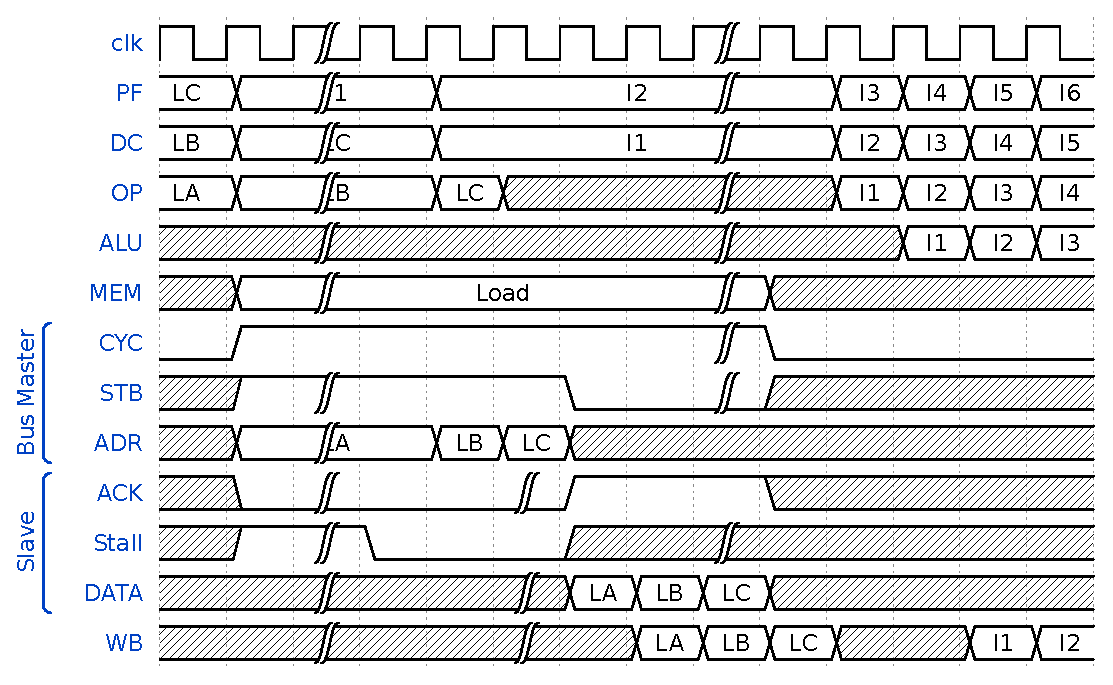
\includegraphics[width=5.6in]{../gfx/memrd.eps}
\caption{Pipeline handling of a load instruction}\label{fig:memrd}
\end{center}\end{figure}
	since it is especially true of a load instruction, which must still
	write its operand back to the register file.  Further, note that on a
	pipelined memory operation, the instruction must stall in the decode
	operand stage, lest it try to read a result from the register file
	before the load result has been written to it.  Finally, note that
	there is an extra stall at the end of the memory cycle, so that
	the memory unit will be idle for two clocks before an instruction will
	be accepted into the ALU.  Store instructions are different, as shown in
	Fig.~\ref{fig:memwr},
\begin{figure}\begin{center}
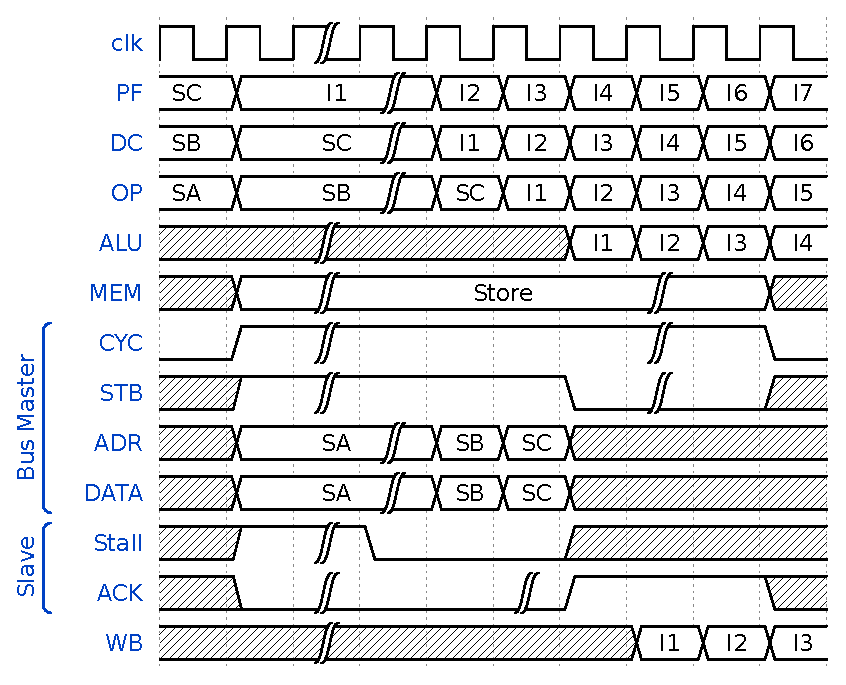
\includegraphics[width=4in]{../gfx/memwr.eps}
\caption{Pipeline handling of a store instruction}\label{fig:memwr}
\end{center}\end{figure}
	since they can be busy with the bus without impacting later write back
	pipeline stages.  Hence, only loads stall the pipeline.

This, of course, also assumes that the memory being accessed is a single cycle
memory and that there are no stalls to get to the memory.
Slower memories, such as the Quad SPI flash, will take longer--perhaps even
as long as forty clocks.   During this time the CPU and the external bus 
will be busy, and unable to do anything else.  Likewise, if it takes a couple
of clock cycles for the bus to be free, as shown in both Figs.~\ref{fig:memrd}
and~\ref{fig:memwr}, there will be stalls.

\item Memory operation followed by a memory operation
\begin{enumerate}
\item\ {\tt SW address,RA}
\item\ {\em (bus dependent number of stalls)}
\item\ {\tt LW address,RB}
\item\ {\em (bus dependent number of stalls)}
\end{enumerate}

	In this case, the LW instruction cannot start until the SW is finished,
	as illustrated by Fig.~\ref{fig:mstld}.
\begin{figure}\begin{center}
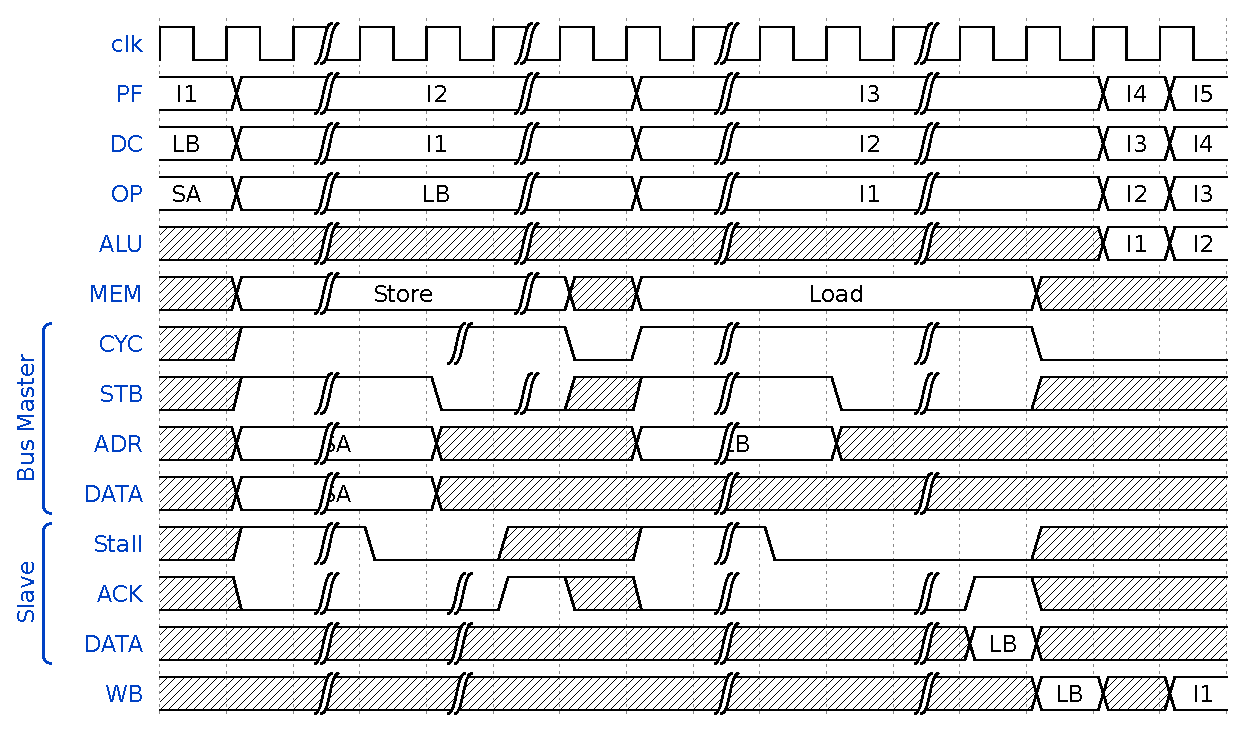
\includegraphics[width=5.5in]{../gfx/mstld.eps}
\caption{Pipeline handling of a store followed by a load instruction}\label{fig:mstld}
\end{center}\end{figure}
	With proper scheduling, it is possible to do something in the ALU
	while the memory unit is busy with the SW instruction, but otherwise
	this pipeline will stall while waiting for it to complete before the
	load instruction can start.

	The ZipCPU has the capability of supporting a form of burst memory
	access, often called pipelined memory access within this document.
	When using this mode, the CPU may issue multiple load or store requests
	at a time, to the extent that all but the first take only a single
	clock.  Doing this requires several conditions to be true:
\begin{enumerate}
\item All accesses within the burst must all be reads or all be writes,
\item All must use the same base register for their address, and
\item There can be no stalls or other instructions between memory
	access instructions within the burst. 
\end{enumerate}
	These conditions work well for saving or storing registers to the stack
	in a burst operation.  Indeed, if you noticed, both
	Fig.~\ref{fig:memrd} and Fig.~\ref{fig:memwr} illustrated pipelined
	memory accesses.
\end{itemize}
%% }}}
\fi

\section{Memory Architecture}
%% {{{
Having now described the CPU registers, instructions, and instruction formats,
we now turn our attention to how the CPU interacts with the rest of the world.
Specifically, we shall discuss how the bus is implemented, and the memory
model assumed by the CPU.

\subsection{Bus Standards}\label{ssec:bus}
%% {{{
The ZipCPU (currently) has the ability to operate using one of three bus types:
Wishbone (B4, pipelined), AXI-Lite, or AXI (full).

When using Wishbone, several choices have been made to simplify this bus.
First, all unnecessary ancillary information has been removed.  This includes
the retry, tag, lock, cycle type indicator, and burst indicator signals.
Second, we insist that all accesses be pipelined.  As a result, Wishbone
transactions complete whenever either the ERR line goes high or the last ACK
has been received.

Further, the ZipCPU is big endian in how it uses the bus.

This becomes a problem when using either AXI-Lite and AXI (full) bus standards,
since these standards are specifically little endian.  In general, this isn't
a problem for the instruction fetch since all instructions are 32-bit
words--the words are just ordered so that the MSB stays the MSB regardless of
byte order.  Things become more difficult for data accesses.  Even though the
ZipCPU data bus components can naturally handle the AXI bus in the required
little-endian fashion, the tool chain doesn't yet fully support this.  Where
this difference becomes a problem is when accessing peripherals.  The AXI
specification requires that any big-endian CPU re-order all of its bytes to
access a 32-bit peripheral.  This would force the CPU to need to rearrange
all of the bytes from big to little endian byte order in any 32-bit peripheral
access, and would therefore likewise require a change to all 32-bit
peripherals so that they would reorder their bytes back to their natural order.

To avoid needing to rearrange all bus accesses in software, the ZipCPU's
various AXI memory components have been written with a {\tt SWAP\_WSTRB} option.
When using {\tt SWAP\_WSTRB}, bytes within a 32-bit word are left in their
natural order contrary to the AXI specification.  32-bit writes maintain their
MSB to LSB order, from left to write, as do 16-bit writes.  This is contrary
to the AXI specification.  However, it allows the ZipCPU to interact with
32-bit peripherals using the ZipCPU's natural byte-order.  Sadly, this means
that, when interacting with a memory type of peripheral--specifically when
interacting with DMAs of any type, then either all components must be adjusted
to use this (non-)standard, or the CPU must re--order bytes within 32-bit words
in software.
%% }}}
\subsection{Memory Model}\label{ssec:memory}
%% {{{
The memory model of the ZipCPU is that of a uniform 32--bit address space.
The CPU knows nothing about which addresses reference on--chip or off-chip
memory, or even which addresses reference peripherals (outside of the data
cache).  There are two exceptions to this memory model.  The first exception
is that the data cache needs to be able to know what addresses can be
cached and which ones cannot be cached.  The bus compositor must therefore
create an {\em iscachable.v} module that the data cache can reference to
know what addresses can be cached.  This module examines addresses, and
returns a bit indicating if values at the given address can be cached.
The second exception applies to the ZipSystem CPU wrapper.  When using this
wrapper, memory addresses where the most significant 8--bits of 32
are set are reserved for processor local peripherals.  These local
peripherals will be discussed more in Sec.~\ref{chap:accessory}.  Other
bus wrappers will forward these addresses directly to memory.

The prefetch cache currently has no means of detecting whether instruction
memory gets changed outside of the CPU.  As a result, any DMA operation should
be followed by a manual clearing the instruction and data caches.  This may
be necessary when loading programs into previously used memory, or when
creating self--modifying code.

Should the memory management unit (MMU) be integrated into the ZipCPU, the MMU
configuration will replace the {\em iscachable} module and tell the ZipCPU
wich addresses may be cached and which not.

This topic is discussed further in the linker section, Sec.~\ref{sec:ld-mem}
of the ABI chapter, Chap.~\ref{chap:abi}.

% \subsection{Measured Performance}\label{sec:perf}
%% }}}
%% }}}
\section{Debug Interface}\label{sec:debug}
%% {{{
The ZipCPU supports an external debug port.  This port has a minimum of
64~word address locations.  Using this interface, it is possible to both
control the CPU, as well as read register values and current status from the
CPU.

While a more detailed discussion will be reserved for Sec.~\ref{sec:reg-debug},
here we'll just discuss how it is put together.  The debug interface allows
a controller access to the CPU reset signal, a halt control signal, and a
clear cache request signal.  By raising the reset line, the CPU will be caused
to clear it's cache, to clear any internal exception or error conditions, and
then to start execution at the {\tt RESET\_ADDRESS}.  This will cause the
CPU to reboot, while only forcing changes to the CC and PC registers.  In a
similar fashion, the debug interface allows you to control the {\tt cpu\_halt}
line into the CPU.  Holding this line high will hold the CPU in an externally
halted state.  Toggling the line low for one clock allows one to step the CPU
by one instruction.  Lowering the line causes the CPU to go.  The final control
wire, controlled by the debug interface, will force the CPU to clear its cache.
All of these control wires are set or cleared from the external debug control
register.  This control register occupies the zero address of the
ZipCPU's debug register space, and aliases to the next 31 addresses.

The other 32-word addresses are allocated to the various ZipCPU registers,
starting with the supervisor registers.  This means that a debugger can first
halt the CPU and then examine or even modify its full register set, before
telling the CPU to continue.

One of the big differences between version~2 and version~3 of the ZipCPU
are the address allocations for these registers.  In previous versions of
the ZipCPU, reading CPU register state required writing the register's
address to the control register before reading the register's value back.
This proved to be problematic when trying to debug the ZipCPU over a slow
link.  By creating a separate address for each register, burst read requests
may be issued by the debugger for the entire register state.  This can
greatly speed up interactions between the debugger and the CPU.

Finally, without halting the CPU, the debug controller can read from any
single register, and it can see if the CPU is still actively running, whether
it is in user or supervisor modes, and whether or not it is sleeping.  This
alone is useful for detecting deadlocks or other difficult problems.
%% }}}
%% }}}
\chapter{Operation}\label{chap:ops}
%% {{{
This chapter will explore how to perform common tasks with the ZipCPU,
offering examples in both C and assembly for those tasks.

\section{CRT0}
%% {{{
Of course, the one task that every CPU must do is start the CPU for other
tasks.  The ZipCPU is no different.  This is the one ZipCPU task that must
take place in assembly, since no assumptions can be made about the state of
the ZipCPU upon entry.  In particular, the stack pointer, SP, needs to be
loaded with a valid memory location before any higher level language can work.
Once that has taken place, it is then possible to call other higher level
routines.

Table.~\ref{tbl:op-init}
\begin{table}\begin{center}
\begin{tabbing}
{\em ; By starting our loader in the .start section, we guarantee through our}\\
{\em ; linker script that these are the very first instructions the CPU sees.}\\
\hbox to 0.25in{}\={\tt .section .start} \\
\>	{\tt .global \_start} \\
{\em ; \_start is to be placed at our reboot/reset address, so it will be}\\
{\em ; called upon any reboot.}\\
{\tt \_start:} \\
%
%
\> {\em ; The most important step: creating a stack pointer.  The value}\\
\> {\em ; {\tt \_top\_of\_stack} is created by the linker based upon the linker script.}\\
\>	{\tt LDI \_top\_of\_stack,SP} \\
%
%
\> {\em ; We then call the bootloader to load our code into memory.}\\
\>	{\tt MOV \_after\_bootloader(PC),R0} \\
\>	{\tt BRA bootloader} \\
{\tt \_after\_bootloader:} \\
%
%
\>	{\em ; Clear the cache, so any DMA operations will be recognized.}\\
\>	{\tt OR	0xc000,CC} \\
%
\>	{\em ; Set argc to zero}\\
\>	{\tt CLR	R1} \\
\>	{\em ; Point argv to NULL}\\
\>	{\tt MOV	\_argv(PC),R2} \\
\>	{\em ; A pointer to the environment (often NULL)}\\
\>	{\tt LDI	\_\_env,R3} \\
%
%
\>	{\em ; Finally, we call the main function.}\\
\>	{\tt JSR	main}\\
%
%
{\em ; Call the C-library exit function}\\
{\em ; If main falls through, then the user hasn't done so, so call it here.}\\
{\em ; exit() should not return.}\\
{\tt \_graceful\_kernel\_exit:} \\
\>	{\tt JSR	exit}\\
%
{\em ; The library exit() function should call \_hw\_shutdown() on completion.}\\
{\em ; Any ongoing hardware operations should have ended before now}\\
\>	{\tt .global \_hw\_shutdown} \\
{\tt \_hw\_shutdown:} \\
\>	{\tt NEXIT}\\
%
%
{\em ; Finally, we halt the CPU }\\
{\tt \_kernel\_is\_dead:}\\
\>	{\tt HALT}\\
\>	{\em ; Just in case \ldots}\\
\> {\tt BRA \_kernel\_is\_dead}
{\em ; Provide a dummy value for an empty argv list}\\
{\tt \_argv:} \\
\> {\tt .WORD	0,0}
\end{tabbing}
\caption{Setting up a stack frame and starting the CPU}\label{tbl:op-init}
\end{center}\end{table}
presents an example of one such initialization routine
that first sets up the stack, then calls a bootloader routine to potentially
copy program memory from ROM to RAM and zero out any global memory space.
Upon completion, the initialization routine then calls main.  Should
main ever return, this routine will call exit.  Finally, once exit completes,
a short routine following halts the CPU.

% \section{Example bootloader}
%% }}}
\section{System High}
%% {{{
The easiest and simplest way to run the ZipCPU is just to leave it in its
supervisor mode, herein called ``System High.'' In this mode, the CPU runs
your program in supervisor mode from reset to power down, and is never
interrupted.  You will need to poll the interrupt controller to determine when
any external condition has become active.  This mode is incredibly useful, and
can handle many microcontroller--type tasks. 

Even better, in system high mode, all of the user registers are available
to the system high program as variables.  Accessing these registers can be
done in a single clock cycle, which would move them to the active register
set or move them back.  While this may seem like a load or store instruction,
none of these register accesses will suffer from memory delays.

While supervisor mode tasks cannot be interrupted, they can wait for
interrupts via the {\tt WAIT} instruction.  This instruction can be accessed
from C using the {\tt zip\_wait()} built--in function.  This will place the
ZipCPU into an idle/sleep mode to wait for interrupts.  Because the
supervisor puts the CPU to sleep, rather than the user, no user context
needs to be set up.
%% }}}
\section{A Programmable Delay}
%% {{{
One common task in microcontrollers, whether in a user task or supervisor
task, is to wait for a programmable amount of time.  Using the ZipSystem,
there are several peripherals that can be used to create such a delay.
It can be done with any one of the three timers, the ZipJiffies peripheral, or
even an off-chip ZipCounter.

Here, in Tbl.~\ref{tbl:shi-timer},
\begin{table}\begin{center}
\begin{tabbing}
{\tt \#define EINT(A) (0x80008000|(A<<16))} \= {\em // Enable interrupt A}\\
{\tt \#define DINT(A) (A<<16)} \>{\em // Just disable the interrupts in A}\\
{\tt \#define DISABLEALL 0x7fff0000} \>{\em // Disable all interrupts}\\
{\tt \#define CLEARPIC 0x7fff7fff} \>{\em // Clears and disables all interrupts}\\
{\tt \#define SYSINT\_TMA 0x10} \>{\em // The Timer--A interrupt mask}\\
\\
{\tt void timer\_delay(int nclocks) \{} \\
\hbox to 0.25in{}\= {\em // Clear the PIC.  We want to exit from here on timer counts alone}\\
	\> {\tt zip->pic = DISABLEALL|SYSINT\_TMA;}\\
	\> {\tt if (nclocks > 10) \{}\\
	\> \hbox to 0.25in{}\= {\em // Set our timer to count down the given number of counts}\\
	\> \> {\tt zip->z\_tma = nclocks;} \\
	\> \> {\tt zip->z\_pic = EINT(SYSINT\_TMA);} \\
	\> \> {\tt zip\_wait();} \\
	\> \> {\tt zip->z\_pic = CLEARPIC;} \\
	\> {\tt \} }{\em // else anything less has likely already passed} \\
{\tt \}}\\
\end{tabbing}
\caption{Waiting on a timer}\label{tbl:shi-timer}
\end{center}\end{table}
we present one means of waiting for a programmable amount of time using a
timer.  If exact timing is important, you may wish to calibrate the method
by subtracting from the counts number the counts it takes to actually do the
routine.  Otherwise, the timer is guaranteed to at least {\tt counts}
ticks.

Notice that the routine clears the PIC early on.  While one might expect
that this could be done in the instruction immediately before {\tt zip\_rtu()},
this isn't the case.  The reason is a race condition created by the fact that
the write to the PIC might complete after the {\tt zip\_rtu()} instruction.
(Remember, the ZipCPU doesn't wait for write completion before issuing its
next instruction.)  As a result, you might find yourself with a zero delay
simply because the timer had tripped some time earlier.  An alternative way
of dealing with this is to read from the PIC after writing to it.

The routine is also careful not to clear any other interrupts beyond the timer
interrupt, lest some other condition trip that the user was also waiting on.
%% }}}
\section{Traditional Interrupt Handling}
%% {{{
Although the ZipCPU does not have a traditional interrupt vector architecture,
with interrupt vector addresses kept somewhere in memory, it is still
possible to create the more traditional interrupt approach via software.
In this mode, the programmable interrupt controller is used together with the
supervisor state to create the illusion of more traditional interrupt handling.

To set this up, upon reboot the supervisor task:
\begin{enumerate}
\item Creates a (single) user context, a user stack, and sets the user
	program counter to the entry of the user task
\item Creates a task table of ISR entries
\item Enables the master interrupt enable via the interrupt controller, albeit
	without enabling any of the fifteen potential underlying interrupts.
\item Switches to user mode, as the first part of the while loop in 
	Tbl.~\ref{tbl:traditional-isr}.
\end{enumerate}
\begin{table}\begin{center}
\begin{tabbing}
{\tt while(true) \{} \\
\hbox to 0.25in{}\= {\tt zip\_rtu();}\\
	\> {\tt if (zip\_ucc() \& CC\_TRAPBIT) \{} {\em // Here, we allow users to install ISRs, or} \\
	\>\hbox to 0.25in{}\= {\em // whatever else they may wish to do in supervisor mode.} \\
	\>\> {\tt \ldots} \\
	\> {\tt \} else (zip\_ucc() \& (CC\_BUSERR|CC\_FPUERR|CC\_DIVERR)) \{}\\
	\>\> {\em // Here we handle any faults that the CPU may have
		encountered }\\
	\>\> {\em // The easiest solution is often to print a trace and reboot}\\
	\>\> {\em // the CPU.}\\
	\>\> {\tt \_start();} \\
	\> {\tt \} else \{} \\
	\> \> {\em // At this point, we know an interrupt has taken place:  Ask the programmable}\\
	\> \> {\em // interrupt controller (PIC) which interrupts are enabled and which are active.}\\
	\> \>	{\tt int	picv = zip->pic;}\\
	\> \>	{\em // Turn off all active interrupts}\\
	\> \>	{\tt int	active = (picv >> 16) \& picv \& 0x07fff;}\\
	\> \>	{\tt zip->pic = (active<<16);}\\
	\> \>	{\em // We build a mask of interrupts to re-enable in picv.}\\
	\> \>	{\tt picv = 0;}\\
	\> \>	{\tt for(int i=0,msk=1; i<15; i++, msk<<=1) \{}\\
	\> \>\hbox to 0.25in{}\={\tt if ((active \& msk)\&\&(isr\_table[i])) \{}\\
	\> \>\>\hbox to 0.25in{}\={\em // Here we call our interrupt service routine.}\\
	\> \>\>\hbox to 0.25in{}\= {\tt (isr\_table[i])(); }\\
	\> \>	{\tt \} }\\
	\>{\tt \} }\\
{\tt \}}\\
\end{tabbing}
\caption{Traditional Interrupt handling}\label{tbl:traditional-isr}
\end{center}\end{table}

We can work through the interrupt handling process by examining
Tbl.~\ref{tbl:traditional-isr}.  First, remember, the CPU is always running
either the user or the supervisor context.  Once the supervisor switches to
user mode, control does not return until either an interrupt, a trap, or an
exception has taken place.  Therefore, if neither the trap bit nor any of the
exception bits have been set, then we know an interrupt has taken place.

It is also possible that an interrupt will occur coincident with a trap or
exception.  If this is the case, the subsequent {\tt zip\_rtu()} instruction
will return immediately, since the interrupt has yet to be cleared.

As Sec.~\ref{sec:pic} discusses, the top of the PIC register stores which 
interrupts are enabled, and the bottom stores which have tripped.  (Interrupts
may trip without being enabled, they just will not generate an interrupt to the
CPU.)  Our first step is to query the register to find out our interrupt
state, and then to disable any interrupts that have tripped.  To do
that, we write a one to the enable half of the register while also clearing
bit fifteen--creating a disable interrupt command.

Using the bit mask of interrupts that have tripped, we walk through all fifteen
possible interrupts.  If there is an ISR installed, we simply call it here.

There you have it: the ZipCPU, with its non-traditional interrupt architecture,
can still process interrupts in a very traditional fashion. 
%% }}}
\section{Idle Task}
%% {{{
One task every operating system needs is the idle task, the task that takes
place when nothing else can run.  On the ZipCPU, this task is quite simple,
and it is shown in assembly in Tbl.~\ref{tbl:idle-asm},
\begin{table}\begin{center}
\begin{tabbing}
{\tt idle\_task:} \\
\hbox to 0.25in{}\= {\em ; Wait for the next interrupt, then switch to supervisor task} \\
\>        {\tt WAIT} \\
\>        {\em ; When WAIT completes, the CPU will switch to supervisor mode.}\\
\>        {\em ; If the supervisor then re-enables this task, it will be because}\\
\>        {\em ;  the supervisor wishes to wait for an interrupt again.  For}\\
\>        {\em ; this reason, we loop back to the top.} \\
\>        {\tt BRA idle\_task} \\
\end{tabbing}
\caption{Example Idle Task in Assembly}\label{tbl:idle-asm}
\end{center}\end{table}
or equivalently in C in Tbl.~\ref{tbl:idle-c}.
\begin{table}\begin{center}
\begin{tabbing}
{\tt void idle\_task(void) \{} \\
\hbox to 0.25in{}\={\tt while(true) \{} {\em // Never exit}\\
\> {\em // Wait for the next interrupt, then switch to supervisor task} \\

\> {\tt zip\_wait();} \\
\> {\em // } \\
\> {\em // When we come back, it's because the supervisor wishes to} \\
\> {\em // wait for an interrupt again, so go back to the top.} \\
\> {\tt \}} \\
{\tt \}}
\end{tabbing}
\caption{Example Idle Task in C}\label{tbl:idle-c}
\end{center}\end{table}

When this task runs, the CPU will fill up all of the pipeline stages up the
ALU.  The {\tt WAIT} instruction, upon leaving the ALU, places the CPU into
a sleep state where nothing more moves.  Then, once an interrupt takes place,
control passes to the supervisor task to handle the interrupt.  When control
passes back to this task, it will be on the next instruction.  Since that next
instruction sends us back to the top of the task, the idle task thus does
nothing but wait for an interrupt.

This should be the lowest priority task, the task that runs when nothing else
can.  Running this task will reduce power consumption, even stopping the
clock if {\tt OPT\_CLKGATE} is sset.

%% }}}
\section{Context Switch}
%% {{{
Fundamental to any multiprocessing system is the ability to switch from one
task to the next.  In the ZipSystem, this is accomplished in one of a couple of
ways.  The first step is that an interrupt, trap, or exception takes place.
This will pull the CPU out of user mode and into supervisor mode.  At this
point, the CPU needs to execute the following tasks:
\begin{enumerate}
\item Check for the reason, why did we return from user mode?  Did the user
	execute a trap instruction, or did some other user exception such as a
	break, bus error, division by zero error, or floating point exception
	occur.  That is, if the user process needs attending then we may not
	wish to adjust the context, check interrupts, or call the scheduler. 
	Tbl.~\ref{tbl:trap-check}
\begin{table}\begin{center}
\begin{tabbing}
{\tt while(true) \{} \\
	\hbox to 0.25in{}\={\em // The instruction before the context switch processing must} \\
\>	{\em // be the RTU instruction that enacted user mode in the first} \\
\>	{\em // place.  We show it here just for reference.} \\
\>	{\tt zip\_rtu();} \\
\\
\>	{\tt if (zip\_ucc() \& (CC\_FAULT)) \{} \\
\>	\hbox to 0.25in{}\={\em // The user program has experienced an unrecoverable fault and must die.}\\
\>\>	{\em // Do something here to kill the task, recover any resources} \\
\>\>		{\em // it was using, and report/record the problem.}\\
\>\>		\ldots \\
\>	{\tt \} else if (zip\_ucc() \& (CC\_TRAPBIT)) \{} \\
\>\>		{\em // Handle any user request} \\
\>\>		{\tt zip\_restore\_context(userregs);} \\
\>\>		{\em // If the request ID is in uR1, that is now userregs[1]}\\
\>\>		{\tt switch(userregs[1]) \{} \\
\>\>		{\tt case $x$:} {\em // Perform some user requested function} \\
\>\>		\hbox to 0.25in{}\= {\tt break;}\\
\>\>		{\tt \}} \\
\>	{\tt \}}\\
\\
{\tt \}}
\end{tabbing}
\caption{Checking for whether the user task needs our attention}\label{tbl:trap-check}
\end{center}\end{table}
	shows the rudiments of this code, while showing nothing of how the
	actual trap would be implemented.
	
You may also wish to note that the instruction before the first instruction
in our context swap {\em must be} a return to userspace instruction. 
Remember, the supervisor process is re--entered where it left off.  This is
different from many other processors that enter interrupt mode at some vector
or other.  In this case, we always enter supervisor mode right where we last
left.

\item Capture user accounting counters.  If the operating system is keeping
	track of system usage via the accounting counters, the user counters
	need to be copied and accumulated into some master user-task counter
	at this point.

\item Preserve the old context.  This involves recording all of the user
	registers to some supervisor memory structure, such as is shown in
	Tbl.~\ref{tbl:context-out}.
\begin{table}\begin{center}
\begin{tabbing}
{\tt save\_context:} \\
\hbox to 0.25in{}\={\tt SUB 4,SP}\hbox to 0.5in{}\= {\em ; Function prologue: create a stack}\\
\>        {\tt SW R5,(SP)}	\> {\em ; frame and save R5.  (R1-R4 are assumed}\\
\>        {\tt MOV uR0,R2}	\> {\em ; to be used and in need of saving.  Then}\\
\>        {\tt MOV uR1,R3}	\> {\em ; copy the user registers, four at a time to }\\
\>        {\tt MOV uR2,R4}	\> {\em ; supervisor registers, where they can be}\\
\>        {\tt MOV uR3,R5}	\> {\em ; stored, while exploiting memory pipelining}\\
\>        {\tt SW R2,(R1)}	\>{\em ; Exploit memory pipelining: }\\
\>        {\tt SW R3,4(R1)}	\>{\em ; All instructions write to same base memory}\\
\>        {\tt SW R4,8(R1)}	\>{\em ; All offsets increment by one }\\
\>        {\tt SW R5,12(R1)} \\
\>	\ldots {\em ; Need to repeat for all user registers} \\
\>        {\tt MOV uR12,R2}	\> {\em ; Finish copying ... } \\
\>        {\tt MOV uSP,R3} \\
\>        {\tt MOV uCC,R4} \\
\>        {\tt MOV uPC,R5} \\
\>        {\tt SW R2,48(R1)}	\> {\em ; and saving the last registers.}\\
\>        {\tt SW R3,52(R1)}	\> {\em ; Note that even the special user registers }\\
\>        {\tt SW R4,56(R1)}	\> {\em ; are saved just like any others. }\\
\>        {\tt SW R5,60(R1)} \\
\>        {\tt LW (SP),R5}	\> {\em ; Restore our one saved register}\\
\>        {\tt ADD 4,SP}		\> {\em ; our stack frame,} \\
\>        {\tt RETN}		\> {\em ; and return }\\
\end{tabbing}
\caption{Example Storing User Task Context}\label{tbl:context-out}
\end{center}\end{table}
Since this task is so fundamental, the ZipCPU compiler back end provides
the {\tt zip\_save\_context(void *)} function.  

\item Reset the watchdog timer.  If you are using the watchdog timer, it should
	be reset on a context swap, to know that things are still working.

\item Interrupt handling.  How you handle interrupts on the ZipCPU are up to
	you.  You can activate a sleeping task if you like, or for smaller
	faster interrupt routines, such as copying a character to or from a 
	serial port or providing a sample to an audio port, you might choose
	to do the task within the kernel main loop.  The difference may 
	depend upon how you have your hardware set up, how fast the
	kernel main loop is, and how tight your timing requirements are.

\item Calling the scheduler.  This needs to be done to pick the next task
	to switch to.  The next task may be an interrupt handler, or it may
	be a normal user task.  From a priority standpoint, it would make
	sense that the interrupt handlers all have a higher priority than
	the user tasks, and that once they have been called the user tasks
	may then be called again.  If no task is ready to run, run the idle
	task to wait for an interrupt.

	This suggests a minimum of four task priorities:
	\begin{enumerate}
	\item Interrupt handlers, executed with their interrupts disabled
	\item Device drivers, executed with interrupts re-enabled
	\item User tasks
	\item The idle task, executed when nothing else is able to execute
	\end{enumerate}

\item Restore the new tasks context.  Given that the scheduler has returned a
	task that can be run at this time, the user registers need to be
	read from the memory at the user context pointer and then placed into
	the user registers.  An example of this is shown in
	Tbl.~\ref{tbl:context-in},
\begin{table}\begin{center}
\begin{tabbing}
{\tt restore\_context:} \\
\hbox to 0.25in{}\= {\tt SUB 4,SP}\hbox to 0.4in{}\={\em ; Set up a stack frame} \\
\>	{\tt SW R5,(SP)} \> {\em ; and store a local register onto it.}\\
\\
\>	{\tt LW (R1),R2} \> {\em ; By doing four loads at a time, we are }\\
\>	{\tt LW 4(R1),R3} \> {\em ; making sure we are using our pipelined}\\
\>	{\tt LW 8(R1),R4} \> {\em ; memory capability. }\\
\>	{\tt LW 12(R1),R5} \\
\>	{\tt MOV R2,uR1} \> {\em ; Once the registers are loaded, copy them }\\
\>	{\tt MOV R3,uR2} \> {\em ; into the user registers that they need to}\\
\>	{\tt MOV R4,uR3} \> {\em ; be placed within.} \\
\>	{\tt MOV R5,uR4} \\
	\> \ldots {\em ; Need to repeat for all user registers} \\
\>	{\tt LW 48(R1),R2} \> {\em ; Now for our last four registers ...}\\
\>	{\tt LW 52(R5),R3} \\
\>	{\tt LW 56(R5),R4} \\
\>	{\tt LW 60(R5),R5} \\
\>	{\tt MOV R2,uR12} \> {\em ; These are the special purpose ones, restored }\\
\>	{\tt MOV R3,uSP} \> {\em ; just like any others.}\\
\>	{\tt MOV R4,uCC} \\
\>	{\tt MOV R5,uPC} \\

\>	{\tt LW (SP),R5} \> {\em ; Restore our saved register, } \\
\>	{\tt ADD 4,SP}	\> {\em ; and the stack frame, }\\
\>	{\tt RETN}	\> {\em ; and return to where we were called from.}\\
\end{tabbing}
\caption{Example Restoring User Task Context}\label{tbl:context-in}
\end{center}\end{table}
	Because this is such an important task, the ZipCPU GCC provides a
	built--in function, {\tt zip\_restore\_context(void *)}, which can be
	used for this task.  

\item Clear the userspace accounting registers.  In order to keep track of
	per process system usage, these registers need to be cleared before
	reactivating the userspace process.  That way, upon the next
	interrupt, we'll know how many clocks the userspace program has
	encountered, and how many instructions it was able to issue in
	those many clocks. 

\item Return back to the top of our loop in order to execute {\tt zip\_rtu()}
	again.
\end{enumerate}
%% }}}

%% }}}
\chapter{Tool Suite and Application Binary Interface}\label{chap:abi}
%% {{{
This chapter discusses not the CPU itself, but rather how the GCC and binutils
toolchains have been configured to support the ZipCPU.

% ELF Format
% Stack:
%	R13 is the stack register.
%	The stack grows downward.
%	Memory at the current stack pointer is allocated.
%	Hence, a PUSH is : SUB 1,SP; SW Rx,(SP)
% Heap:
%	In general, not yet implemented.  
%	A less than adequate Heap has been implemented as a pointer, from which
%	malloc requests simply decrement it.  Free's are NOOPs, leaving
%	allocated memory allocated forever.

\section{Executable File Format}\label{sec:abi-elf}
ZipCPU executable files are stored in the Executable and Linkable Format
(ELF).  The ZipCPU loader will use this file to load the executable into
flash, or alternatively into whatever memory the program will be executed from.

The ZipCPU described by this specification uses the 16-bits {\tt 16'hdad1}
to identify itself against other CPUs.  This is not an officially registered
number, and may change in the future.

The ZipCPU does not (yet) have a dynamic linker/loader.  All linking is
currently static, and must be done prior to the Zip loader.

\section{Stack}\label{sec:abi-stack}
%% {{{
Register {\tt R13} (also known as the {\tt SP} register) is the stack register.
The compiler generates code that grows the stack from
high addresses to lower addresses.  That means that the stack will usually
start out set to a very large value, such as one past the last RAM address,
and it will grow to lower and lower values--hopefully never mixing with the
heap.  Memory at the current stack position is assumed to be allocated.

When creating a stack frame for a function, the compiler will subtract
the size of the stack frame from the stack register.  It will then store
any registers used by the function, from {\tt R5} to {\tt R12} (including
the link register {\tt R0}) onto offsets given by the stack pointer plus a 
constant.  If a frame pointer is used, the compiler uses {\tt R12} (or
{\tt FP}) for this purpose.  The frame pointer is set by moving the stack
pointer plus an offset into {\tt FP}.  This {\tt MOV} instruction effectively
limits the size of any individual stack frame to $2^{12}-1$ octets.

Once a subroutine is complete, the frame is unwound.  If the frame pointer,
{\tt FP} was used, then {\tt FP} is copied directly to the stack pointer,
{\tt SP}.  Registers are restored, starting with {\tt R0} all the way to
{\tt R12} ({\tt FP}).  This also restores, and obliterates, the subroutine
frame pointer.  Once complete, a value is added to the stack pointer to
return it to its original value, and a jump is made to the value located
within {\tt R0}.
%% }}}
\section{Relocations}\label{sec:abi-reloc}
%% {{{
The ZipCPU binutils back end supports several types of relocations, although
the two most common are the 32--bit relocations for register load and long
jump.

The first of these is for loading an arbitrary 32--bit value into a register. 
Such instructions are broken into a pair of {\tt BREV} and {\tt LDILO}
instructions, and once the value of the parameter is known their immediate
values can be filled in.

The second type of 32--bit relocation is for jumps to arbitrary addresses.
These jumps are supported by the \hbox{\tt LW (PC),PC} instruction, followed
by the 32--bit address to be filled in later by the linker.  If the jump is
conditional, then a conditional \hbox{\tt LW.$x$ 4(PC),PC} instruction is
used, followed by a {\tt ADD 4,PC} and then the 32--bit relocation value.

If a branch distance is known and within reach, then it will be implemented
with an {\tt ADD \#,PC} instruction, possibly conditional, as necessary.

While other relocations are supported, they tend not to be used nearly as much
as these two.
%% }}}
\section{Call format}\label{sec:abi-jsr}
%% {{{
One unique feature of the ZipCPU is that it has no native JSR instruction.
The assembler attempts to minimize this problem by replacing a
{\tt JSR}~{\em address} instruction with a {\tt MOV \#(PC),R0} followed by
a jump to the requested address.  In this case, the offset to the PC for the
{\tt MOV} instruction is determined by whether or not the jump can be
accomplished with a local branch or a long jump.

While this works well in practice, this implementation prevents such things
as {\tt JSR}'s followed by {\tt BRA}'s from being combined together.

Finally, GCC will place first five operands passed to the subroutine into
registers R1--R5, starting with R1.  Any additional operands are placed
upon the stack.
%% }}}
\section{Built-ins}\label{sec:abi-builtin}
%% {{{
The ZipCPU ABI supports the a number of built in functions.  The compiler
maps these functions directly to assembly language equivalents, essentially 
providing the C~programmer with access to several assembly language
instructions.  These are:
\begin{enumerate}
\item {\tt zip\_bitrev(int)} reverses the bits in the given integer, returning
	the result.  This utilizes the internal {\tt BREV} instruction, and is
	designed to be used with FFT's as necessary.
\item {\tt zip\_busy()} executes an {\tt ADD -4,PC} function, essentially
	forcing the CPU into a very tight infinite loop.
\item {\tt zip\_cc()} returns the value of the current CC register.  This may
	be used within both user and supervisor code to determine in which
	mode the CPU is within.
\item {\tt zip\_halt()} executes an \hbox{\tt OR \$SLEEP,CC} instruction to
	place the processor to sleep.  If the processor is in supervisor mode,
	this halts the processor.
\item {\tt zip\_rtu()} executes an \hbox{\tt OR \$GIE,CC} instruction.  This
	will place the CPU into user mode, and has no effect if the CPU is
	already in user mode.
% \item {\tt zip\_step()} executes an \hbox{\tt OR \$STEP|\$GIE,CC} instruction.
%	This will place the CPU into user mode in order to step one instruction,
%	and then return to supervisor mode.
%	It has no effect if the CPU is already in user mode.
\item {\tt zip\_syscall()} executes a \hbox{\tt CLR CC}
	instruction to return the CPU to supervisor mode.  This essentially
	executes a trap, setting the trap bit for the supervisor to examine.

	What this instruction does not do is arrange for the trap arguments to
	be placed into the  registers {\tt R1} through {\tt R5}.  If necessary,
	a function call may be made to an assembly routine that executes the
	trap if necessary to place the arguments in their proper places.

\item {\tt zip\_wait()} executes an \hbox{\tt OR \$SLEEP|\$GIE,CC} instruction.
	Unlike {\tt zip\_halt()}, this {\tt zip\_wait()} instruction places
	the CPU into a wait state regardless of whether or not the CPU is
	in supervisor mode or not.   When this instruction completes, it will
	leave the CPU in supervisor mode upon an interrupt having taken place.

\item {\tt zip\_restore\_context(context *)} inserts the 32~assembly
	instructions necessary to copy all sixteen user registers to a memory
	region pointed to by the given context pointer, starting with {\tt uR0}
	on up to {\tt uPC}.

\item {\tt zip\_save\_context(context *)} inserts the 32~assembly instructions
	necessary to copy all sixteen user registers to a memory region pointed
	to by the given context pointer argument, starting
	with {\tt uR0} on up to {\tt uPC}.
\item {\tt zip\_ucc()}, returns the value of the user CC register.
\end{enumerate}
% Builtin functions:
%	zip_break();
%	zip_syscall(a,b,c,d)
%
%% }}}
\section{Linker Scripts}\label{sec:ld}
%% {{{
The ZipCPU makes no assumptions about its memory layout.  The result, though,
is that the memory layout of a given project is board specific.  This
is accomplished via a board specific linker script.  This section will discuss
some of the specifics of a ZipCPU linker script.

Because the ZipCPU uses a modified binutils package as part of its tool chain,
the format for this linker script is defined by the GNU LD project within
binutils.  Further details on that format may be found within the GNU LD 
documentation within the binutils package.

This discussion will focus on those parts of the script specific to the ZipCPU.

\subsection{Memory Types}\label{sec:ld-mem}
%% {{{
Of the FPGA boards that the ZipCPU has been applied to, most of them have some
combination of three types of memory: flash, block RAM, and (possibly DDR)
Synchronous Dynamic RAM (SDRAM).  Of these three, only the flash is
non--volatile.  The block RAM is the fastest, and the SDRAM the largest.
While other memory types are available, such as files on an external media
such as an SD card or a network drive, these three types have so far been
sufficient for our purposes.

To support these memories, the linker script has three memory lines identifying
where each memory exists on the bus, the size of the memory, and any protections
associated with it.  For example,
\begin{eqnarray*}
\mbox{blkram (wx) : ORIGIN = 0x0008000, LENGTH = 0x0008000}
\end{eqnarray*}
specifies that there is a region of memory, called blkram, that can be read and
written, and that programs can execute from.  This section starts at address
{\tt 0x8000} and extends for another {\tt 0x8000} bytes.  The other memories
are defined in a similar manner, with names {\tt flash} and {\tt sdram}.

Following the memory section, three specific symbols are defined:
\begin{itemize}
\item {\tt \_rom}, defines the beginning of a ROM (i.e. flash) memory area.
	This is the area where software is placed prior to startup.
	It may be set to NULL if the program is already loaded in RAM, and
	doesn't need to be copied to RAM prior to starting.

\item {\tt \_kram}.  Some devices have a faster RAM (i.e. block RAM) than
	others.  {\tt \_kram} defines the location of this RAM.  If not used,
	then this value may be left at NULL.

\item {\tt \_ram}.  This defines the beginning of regular RAM mmeory.
	If both {\tt \_rom} and {\tt \_ram} are defined, then the CRT0
	routine will copy any softare from {\tt \_rom} to {\tt \_ram} on
	startup.
\end{itemize}

These symbols are used to make the bootloader's task easier.
%% }}}
\subsection{The Entry Function}\label{sec:ld-entry}
%% {{{
The ZipCPU has, as a parameter, a {\tt RESET\_ADDRESS}.  It is important
that this address contain a valid instruction (or more), since this is the
first instruction the ZipCPU will execute.  Traditionally, this address is also
the first address in instruction memory as well.

To make this happen, the ZipCPU defines two additional segments: the
{\tt .start} and the {\tt .boot} segments.  The {\tt  .start} segment is to 
have nothing in it but the very initial startup code.  This code typically
needs to run from flash (or other ROM).  It should be placed at the
{\tt RESET\_ADDRESS}.  This is the purpose of the {\tt .start} section--making
sure the {\tt RESET\_ADDRESS} has this function.

The {\tt .boot} section has a similar purpose.  This section includes anything
associated with the bootloader.  It is a special section because, when loading
from flash, the bootloader {\em cannot} be placed in RAM, but must be placed
in flash--since it is the code that loads things from flash into RAM.

It may also make sense to place any code executed once only within flash as
well.  Such code may run slower than the main system code, but by leaving it in
flash it can be kept from consuming any (potentially precious) higher speed
RAM.  To do this, place this other code into the {\tt .boot} section.

You may also find that large data structures that are best left in flash
can also be placed into this {\tt .boot} section as well for that purpose.
%% }}}
\subsection{Bootloader Tags}\label{sec:ld-boot}
%% {{{
The bootloader needs to know a couple things from the linker script.  It needs
to know what code/data to copy to block RAM from the flash, what code/data to
copy to SDRAM, and finally what initial data area needs to be zeroed.  Four
additional pointers, set within a linker script, can define these regions.

\begin{enumerate}
\item {\tt \_kram\_start}

	This is the first location in flash containing data that the bootloader
	needs to move.

\item {\tt \_kram\_end}

	This is a pointer to one past the last location in block RAM to place
	things into.  If this pointer is equal to {\tt \_kram\_start},
	then no information is placed into \_kram.

\item {\tt \_ram\_image\_start}

	This should be equal to one past the last \_kram address, if \_kram
	is used, or alternatively the first address in {\tt \_rom} containing
	data to be copied to the RAM memory area.  By adding the difference
	between {\tt \_ram\_image\_start} and {\tt \_kram} to the flash address
	in {\tt \_kram\_start}, the actual source address within the
	flash of the code/data that needs to be copied into SDRAM can be
	determined.

\item {\tt \_ram\_image\_end}

	This is the ending address of any code/data to be copied into \_ram.
	The distance between this pointer and {\tt \_ram} should be the total
	amount of data to be placed into the RAM memory area.

\item {\tt \_bss\_image\_end}

	The BSS segment contains data the starts with an initial value of
	zero.  Such data are usually not placed in the executable file, nor
	are they placed into any flash image.  This address points to the
	last location in \_ram used by the BSS segment.  The bootloader
	is responsible then for clearing the RAM between
	{\tt \_ram\_image\_end} and {\tt \_bss\_image\_end}.

	The bootloader must also be robust enough to handle the cases where
	1) there is no SDRAM, 2) there is no block RAM (\_kram is NULL), and
	3) where there is non requirement to move memory at all (\_rom is
	NULL)---such as when the program is placed into memory and started
	from there.
\end{enumerate}
\subsection{Other required linker symbols}\label{sec:ld-other}

Two other symbols need to be defined in the linker script, which are used
by the startup code.  These are:
\begin{enumerate}
\item {\tt \_top\_of\_stack}

	This is the address that the startup code will set the stack pointer
	to point to.  It may be one past the last location of a RAM memory,
	whether block RAM or SDRAM.

\item {\tt \_top\_of\_heap}

	This is the first location past the end of the {\tt .bss} segment.
	Equivalently, this is the address of the first unused piece of
	memory.  It is used as the first location from whence to start
	any dynamic memory subsystem.
\end{enumerate}

All of these symbols need to reference word aligned addresses.
%% }}}
%% }}}
\section{Loading ZipCPU Programs}
%% {{{
There are two basic ways to load a ZipCPU program, depending upon whether or
not the ZipCPU is active within the current configuration.  If the ZipCPU
is not a part of the current FPGA configuration, one need only write the 
flash and then switch configurations.  It will be the CPU's responsibility
to place itself in RAM then. 

The more practical alternative is a little more involved, and there are
several steps to it.
\begin{enumerate}
\item Halt the CPU by writing 0x09 to the CPU control register.  This
	both halts and resets the CPU.  It then prevents both bus contention,
	while writing the new instructions to memory, as well as preventing the
	CPU from running some instructions from one program and other
	instructions from another.

\item Load the program into memory.  For many programs this will involve
	loading the program into flash, and necessitate having and using a 
	flash controller.  The ZipCPU also supports being loaded straight into
	RAM address as well, as though the bootloader had completed
	it's task.

\item You may optionally, at this point, clear all of the CPUs registers,
	to make certain the reboot is clean.

\item Set the sPC register to the starting address. 

\item Clear the instruction cache in order to force the CPU to reload its
	cache upon start.

\item Release the CPU by writing a zero to the CPU debug control register.
\end{enumerate}

%% }}}
\section{Starting a ZipCPU program}
\subsection{CRT0}

Most computers have a section of code, conventionally called {\tt crt0}, which
loads a program into memory.  On the ZipCPU, this code starts at {\tt \_start}.
It is responsible for setting the stack pointer, calling the boot loader,
and then calling the main entry function, {\tt entry()}.

Because {\tt \_start} {\em must} be the first symbol in a program, and because
that first symbol is located at the boot address for the CPU, the {\tt \_start}
is placed into the {\tt .start} segment.  It is the only routine placed there.

On those CPU's that don't have enough logic space for a debugger, it may be
useful to place a routine to dump any registers, stack values and/or kernel
traces to an output routine at this time.  That way, on any kernel fault, the
kernel can be brought back up with a debug trace.  This works because rebooting
the CPU doesn't reset any register values save the {\tt sCC} and {\tt sPC}.

\subsection{The Bootloader}

As discussed in Sec.~\ref{sec:ld-boot}, the bootloader must be placed into 
flash if it is used.  It can be a small C program (it need not be assembly,
like {\tt \_start}), and it only needs to copy memory.  First, it copies any
memory from flash to block RAM.  Second, it copies any necessary memory from
flash to SDRAM.  Then, it zeros any memory necessary in SDRAM (or block RAM,
if there is no SDRAM).

These memory copies may be done with the DMA, or they may be done one--at--a
time for a performance penalty.

%% }}}
\chapter{Debug Register Addressing}\label{chap:regs}
%% {{{
This chapter covers the definitions and locations of the ZipCPU's registers
when accessed by the debugging port.  The ZipSystem is special, having access
to an extra set of registers within the same address space, so we'll cover
that separately.

This chapter also marks a significant upgrade from version~2.0 and prior of the
CPU.  In particular, each CPU register has now been given its own address
location in the debug address space.  This should make it easier to read all
registers at once via a burst read command of some type.

\section{Debug Port Registers}\label{sec:reg-debug}
%% {{{
When the ZipCPU has been built with the {\tt OPT\_DBGPORT} parameter set, then
the CPU may be accessed and controlled by an external debug port.  This port
contains at least 64~word addresses, of which 33~are generally assigned.
These registers are shown in Tbl.~\ref{tbl:dbgregs}.
\begin{table}[htbp]
\begin{center}\begin{reglist}
ZIPCTRL & 0 & 32 & R/W & ZipCPU Control and Status Register \\\hline
\vdots & \vdots & &  & (Reserved addresses)\\\hline
sR0 & 128 & 32 & R/W & Supervisor Register R0 \\\hline
sR1 & 132 & 32 & R/W & Supervisor Register R1 \\\hline
\vdots & \vdots & 32 & R/W & Other supervisor registers\\\hline
sSP & 180 & 32 & R/W & Supervisor Stack Pointer\\\hline
sCC & 184 & 32 & R/W & Supervisor Condition Code Register \\\hline
sPC & 188 & 32 & R/W & Supervisor Program Counter\\\hline
uR0 & 192 & 32 & R/W & User Register R0 \\\hline
uR1 & 196 & 32 & R/W & User Register R1 \\\hline
\vdots & \vdots & 32 & R/W & Other user registers\\\hline
uSP & 244 & 32 & R/W & User Stack Pointer\\\hline
uCC & 248 & 32 & R/W & User Condition Code Register \\\hline
uPC & 252 & 32 & R/W & User Program Counter\\\hline
\end{reglist}
\caption{ZipSystem Debug Registers}\label{tbl:dbgregs}
\end{center}\end{table}
The ZipSystem wrapper contains an additional 64~words as well, which we'll get
to in a moment.

The foremost register among these is the ZipCPU Control and Status Register.
This register has the fields shown in
Tbl.~\ref{tbl:dbgctrl}.
\begin{table}\begin{center}
\begin{bitlist}
11 & RO & The CPU has suffered from a break condition, and has halted itself
	as a result.\\\hline
10 & RO & True if an interrupt is pending.\\\hline
9 & RO & GIE.  If set, the CPU is currently in user mode.\\\hline
8 & RO & Sleep.  The CPU is sleeping.\\\hline
7--6 & & (Reserved)\\\hline
5 & R/W & Debug catch bit.  If set to `1', then the CPU will halt on any
	external exception.  Otherwise, the CPU will reboot on any
	exception.\\\hline
4 & WO & Clear cache.  Set to `1' to clear both the CPU's caches and its
	pipelines.  This is useful if you have just adjusted memory and now
	  need the CPU to be able to read that adjusted memory.
	As a side effect, setting this bit will also halt the CPU if it wasn't
	  halted before.
	\\\hline
3 & R/W & Reset.  Set to `1' to reset the CPU.  If the CPU has been configured
	to start in a halted state, it will reset and then halt.\\\hline
2 & WO & Step Command.  Set to `1' to step the CPU, and then leave it halted.
	Self clearing.\\\hline
1 & RO & Halt status.  If true, the CPU has come to a complete halt.\\\hline
0 & R/W & Halt request.  Set to `1' to halt the CPU.\\\hline
\end{bitlist}
\caption{Debug Control Register Bits}\label{tbl:dbgctrl}
\end{center}\end{table}

Here are some operations you can do with this register:

\begin{enumerate}
\item Reset: To reset the CPU, write an {\tt 0x08} to the debug control
	register.  If the CPU was configured to immediately start on reset,
	then the CPU will start immediately.  If not, a second write will
	be required to release the CPU.

\item Reset and halt: To reset the CPU but leave it halted, write a
	{\tt 0x09} to the debug control register.

\item Start a halted CPU: If the CPU is halted, simply write a {\tt 0x00}
	to the debug control register in order to cause it to continue.

\item Stepping the CPU: To step through a single instruction, write a
	{\tt 0x04} to the debug control register.  This will step one
	instruction through the CPU and then halt it again immediately
	following that instruction.

	The CPU will not step through compound instructions or LOCK
	instruction sequences, but rather it will step over them as though
	they were only a single instruction.  Hence, any compound instruction
	will continue until both instructions have been executed (or one
	trapped).  Similarly, a LOCK instruction will step the full four
	instructions sequence before halting.

\item Halting the CPU.  To halt the CPU, simply write a {\tt 0x01} to the
	debug control register.  Once the register reads back a {\tt 0x03}, the
	CPU is halted.

\end{enumerate}

Debug port reads from these internal register addresses will return the
current value from the CPU's internal register set.  If the CPU is still
running, the value returned may be out of date as soon as it is returned.
For this reason, it makes sense to halt the CPU first.

On the other hand, any attempt to write to an internal CPU register will
require that the CPU first be halted.  This is accomplished in the wrapper
processing the request.  Such writes will also leave the CPU in a halted
state.

\subsection{Breakpoint Handling}
%% {{{

Breakpoints can be handled via the debug control register.  Once a breakpoint
has been hit, the CPU will halt, raise its external interrupt flag, and
set the break bit in the debug control register.

At this point, the debugger may examine and/or modify any registers as
necessary.

Once complete, the breakpoint instruction may be replaced with another
instruction, the cache cleared, and that instruction may then be stepped
through.  The breakpoint may then be replaced and the cache cleared again.
The CPU may then be started to go until its next breakpoint.
%% }}}
%% }}}
\section{ZipSystem Registers}
%% {{{

The ZipSystem has an additional set of registers which may be accessed by
the CPU.  These are associated with the additional peripherals the ZipSystem
wrapper provides to the CPU.  These registers are listed in
Tbl.~\ref{tbl:dbgaddrs}.
\begin{table}\begin{center}
\begin{reglist}
PIC    & 256 & 32 & R/W & Primary Interrupt Controller \\\hline
WDT    & 260 & 32 & R/W & Watchdog Timer\\\hline
WBUS   & 264 & 32 & RO  & Address of the Last Bus Error\\\hline
APIC  & 268 & 32 & R/W & Secondary Interrupt Controller\\\hline
TMRA   & 272 & 32 & R/W & Timer A\\\hline
TMRB   & 276 & 32 & R/W & Timer B\\\hline
TMRC   & 280 & 32 & R/W & Timer C\\\hline
JIFF   & 284 & 32 & R/W & Jiffies peripheral\\\hline
MTASK  & 288 & 32 & R/W & Master task clock counter\\\hline
MMSTL  & 292 & 32 & R/W & Master memory stall counter\\\hline
MPSTL  & 296 & 32 & R/W & Master Pre-Fetch Stall counter\\\hline
MICNT  & 300 & 32 & R/W & Master instruction counter\\\hline
UTASK  & 304 & 32 & R/W & User task clock counter\\\hline
UMSTL  & 308 & 32 & R/W & User memory stall counter\\\hline
UPSTL  & 312 & 32 & R/W & User Pre-Fetch Stall counter\\\hline
UICNT  & 316 & 32 & R/W & User instruction counter\\\hline
DMACMD & 320 & 32 & R/W & DMA command and status register\\\hline
DMALEN & 324 & 32 & R/W & DMA transfer length\\\hline
DMASRC & 328 & 32 & R/W & DMA read address\\\hline
DMADST & 332 & 32 & R/W & DMA write address\\\hline
\end{reglist}
\caption{Debug Register Addresses}\label{tbl:dbgaddrs}
\end{center}\end{table}
These registers addresses allow an external debugger to have access to the
ZipSystem peripherals as well as the CPU register set.  These peripherals
may be read or written from the debug data port.

In this manner, the ZipSystem's full internal state may be read and adjusted,
in addition to the CPU's internal register state.
%% }}}
%% }}}
\chapter{ZipSystem Peripherals}\label{chap:accessory}
%% {{{
The ZipSystem CPU wrapper contains a minimal CPU peripheral set which can be
accessed internally.  Here in this section, we'll walk through the definition
of each of these registers in turn, together with any bit fields that may be
associated with them, and how to set those fields.

The registers themselves can be found at the address shown in
Fig.~\ref{tbl:zpregs}.
\begin{table}[htbp]
\begin{center}\begin{reglist}
PIC   & \scalebox{0.8}{\tt 0xff000000} & 32 & R/W & Primary Interrupt Controller \\\hline
WDT   & \scalebox{0.8}{\tt 0xff000004} & 32 & R/W & Watchdog Timer \\\hline
WBU   &\scalebox{0.8}{\tt 0xff000008}  & 32 & RO  & Address of last bus error\\\hline
APIC & \scalebox{0.8}{\tt 0xff00000c} & 32 & R/W & Secondary Interrupt Controller \\\hline
TMRA  & \scalebox{0.8}{\tt 0xff000010} & 32 & R/W & Timer A\\\hline
TMRB  & \scalebox{0.8}{\tt 0xff000014} & 32 & R/W & Timer B\\\hline
TMRC  & \scalebox{0.8}{\tt 0xff000018} & 32 & R/W & Timer C\\\hline
JIFF  & \scalebox{0.8}{\tt 0xff00001c} & 32 & R/W & Jiffies \\\hline
MTASK & \scalebox{0.8}{\tt 0xff000020} & 32 & R/W & Master Task Clock Counter \\\hline
MMSTL & \scalebox{0.8}{\tt 0xff000024} & 32 & R/W & Master Stall Counter \\\hline
MPSTL & \scalebox{0.8}{\tt 0xff000028} & 32 & R/W & Master Pre--Fetch Stall Counter \\\hline
MICNT & \scalebox{0.8}{\tt 0xff00002c} & 32 & R/W & Master Instruction Counter\\\hline
UTASK & \scalebox{0.8}{\tt 0xff000030} & 32 & R/W & User Task Clock Counter \\\hline
UMSTL & \scalebox{0.8}{\tt 0xff000034} & 32 & R/W & User Stall Counter \\\hline
UPSTL & \scalebox{0.8}{\tt 0xff000038} & 32 & R/W & User Pre--Fetch Stall Counter \\\hline
UICNT & \scalebox{0.8}{\tt 0xff00003c} & 32 & R/W & User Instruction Counter\\\hline
DMACTRL& \scalebox{0.8}{\tt 0xff000040} & 32 & R/W & DMA Control Register\\\hline
DMALEN & \scalebox{0.8}{\tt 0xff000044} & 32 & R/W & DMA total transfer length\\\hline
DMASRC & \scalebox{0.8}{\tt 0xff000048} & 32 & R/W & DMA source address\\\hline
DMADST & \scalebox{0.8}{\tt 0xff00004c} & 32 & R/W & DMA destination address\\\hline
\end{reglist}
\caption{ZipSystem Internal/Peripheral Registers}\label{tbl:zpregs}
\end{center}\end{table}
These registers are all 32-bit registers.  Writes of less than 32--bits
may have unexpected results.  Further, they are located in a reserved location
within the CPU's address space.  As a result, references to these locations
by either a ZipBones or an AXI based system may generate a bus error.  When
using the AXI bus, a separate AXI-lite peripheral set is available to offer
all but the DMA's capability.  However, the AXI-lite peripheral set is not
guaranteed to be in any particular address location.

Here in this section, we'll walk through the definition of each of these
registers/peripherals in turn, together with any bit fields that may be
associated with them, and how to set those fields.

\section{Interrupt Controller(s)}\label{sec:pic}
%% {{{
Perhaps the most important peripheral within the ZipSystem is the interrupt
controller.  While the ZipCPU itself can only handle one interrupt, and has
only the one interrupt state: disabled or enabled, the interrupt controller
can make things more interesting.

The ZipSystem interrupt controller module supports up to 15 interrupts, all
controlled from one register.  Further, it has been designed so that individual
interrupts can be enabled or disabled individually without having any knowledge
of the rest of the controller setting.  To enable an interrupt, write to the
register with bit 15 set and the respective interrupt
enable bit set.  No other bits will be affected.  To disable an interrupt,
write to the register bit 15 clear and the
respective interrupt enable bit set.  To clear an interrupt, write a `1' to
that interrupt's status bit.  The interrupt enable pin for the global interrupt
enable is set and cleared likewise.

As an example, suppose you wished to enable interrupt \#4.  You would then
write to the register a {\tt 0x80108010} to enable interrupt \#4, interrupts
in general, and to clear any past active state for interrupt \#4.  When you
later wish to disable this interrupt, you would write a {\tt 0x00100010} to
the register.  This both disables the interrupt and clears the active
indicator.  This does not disable interrupts in general, however.  To do that
you'd also need to set bit 31.  Similarly a subsequent write of
{\tt 0x80000000} will disable all interrupts as well.  (Why?  Bit 31 selects
the global interrupt enable, and bit 15 is clear meaning that the interrupts
will be disabled.)

The ZipSystem hosts two interrupt controllers: a primary and a secondary.  The
primary interrupt controller is the one that interrupts the CPU.  It has
six local interrupt lines, the rest coming from external interrupt sources.
One of those interrupt lines to the primary controller comes from the secondary
interrupt controller.  This controller maintains an interrupt state for the
process accounting counters, and any other external interrupts that didn't fit
into the primary interrupt controller.

As a word of caution, because the interrupt controller is an external
peripheral, and because memory writes take place concurrently with any following
instructions, any attempt to clear interrupts on one instruction followed by
an immediate Return to Userspace ({\tt RTU}) instruction, may not have the
effect of having interrupts cleared before the {\tt RTU} instruction executes.
This is only relevant if the two instructions take place in immediate
succession.  As an alternative, reading from the interrupt controller after
writing to it will place enough time between these two events for the
{\tt RTU} command to successfully complete.

Looking into the bits that define this controller, you can see from
Tbl.~\ref{tbl:picbits},
\begin{table}\begin{center}
\begin{bitlist}
31 & R/W & Master Interrupt Enable\\\hline
30\ldots 16 & R/W & Interrupt Enable lines\\\hline
15 & R & Current Master Interrupt State\\\hline
15 & W & Set to `1' when writing to the device in order to enable any
	interrupt lines whose respective bits are set in bits 16-31, `0'
	to clear them\\\hline
15\ldots 0 & R/W & Input Interrupt states, write `1' to clear\\\hline
\end{bitlist}
\caption{Interrupt Controller Register Bits}\label{tbl:picbits}
\end{center}\end{table}
that the ZipCPU Interrupt controller has five different types of bits.
The high order bit, or bit--31, is the master interrupt enable bit.  When this
bit is set, then any time an interrupt occurs the CPU will be interrupted and
will switch to supervisor mode, etc.

The CPU also has a global interrupt enable bit defined internally as well.  This
bit is separate from the master interrupt enable in the programmable interrupt
controller.  Both the PICs master interrupt enable and the CPU's global
interrupt enable bit (turning on user mode) will both need to be set for
interrupts to be received and processed.

Bits 30~\ldots 16 of the PIC are individual interrupt enable bits.  Should the
respective interrupt line ever be high while its enable line is also high and
while the master enable line is high, an interrupt will be generated.  Further,
interrupts are level triggered.  Hence, if the interrupt is cleared while the
line feeding the controller remains high, then the interrupt will re--trip.
To set one of these interrupt enable bits, one needs to write to the
controller while both writing a `1' to this bit and a `1' to bit 15.
To clear the bit later, one need only write a `1' to this enable bit,
while leaving bit 15 low.  

Bits 14\ldots 0 are the current state of the interrupt vector.  Interrupt lines
trip whenever they are high, and remain tripped until the input is lowered and
the interrupt is acknowledged.  To lower an interrupt line, simply write a one
to the active interrupt bit to acknowledge it.  Since interrupts are level
triggered, this will only clear the line if the incoming interrupt has also
been cleared.  For this reason, it makes sense to clear the interrupt first
in the peripheral generating it, and then in the interrupt controller.

As an example, consider the following scenario where the ZipCPU supports four
interrupts, 3\ldots0.
\begin{enumerate}
\item The Supervisor will first, while in the interrupts disabled mode,
	write a {\tt 32'h800f800f} to the controller.  This will enable the
	master interrupt line, as well as interrupts 0-3 while also clearing any
	past status from interrupts 0-3.  The supervisor may then
	switch to the user mode to fully enable interrupts.
\item When an interrupt occurs, the CPU will switch to the supervisor mode.
	It may then cycle through the interrupt bits to learn which
	interrupt handler to call.
\item If the interrupt handler expects more interrupts, it will clear its
	current interrupt line when it is done handling the interrupt in
	question.  To do this, it will write a `1' to the low order interrupt
	mask, such as writing a {\tt 32'h0000\_0001}.
\item If the interrupt handler does not expect any more interrupts, it will
	instead clear the interrupt from the controller by writing a 
	{\tt 32'h0001\_0001} to the controller.
\item The supervisor should also check for any user exceptions here,
	but this action has nothing to do with the interrupt control
	register itself.
\item The CPU may then leave supervisor mode, possibly adjusting
	whichever task is running, by executing a return to userspace
	instruction.
\end{enumerate}
%% }}}
\subsection{Timer Register}\label{sec:reg-timer}
%% {{{
The ZipSystem contains three separate timer registers.  Each has an identical
functionality, and a single control and status register whose bit definitions
are given in Tbl.~\ref{tbl:tmrbits}.
\begin{table}\begin{center}
\begin{bitlist}
31 & R/W & Auto-Reload\\\hline
30\ldots 0 & R/W & Current timer value\\\hline
\end{bitlist}
\caption{Timer Register Bits}\label{tbl:tmrbits}
\end{center}\end{table}
This is a very simple timer.  It just counts down to zero and then trips an
interrupt.  Writing to the current timer value sets the value to count down
from, and reading from it returns that value.  Writing to the current timer
value while also setting the auto--reload bit will send the timer into an
auto--reload mode.  In this mode, upon setting its interrupt bit for one
cycle, the timer will also reset itself back to the value of the timer
that was written to it when the auto--reload option was written to it.  To
clear and stop the timer, just simply write a `32'h00' to this register.

This timer may be used for non--interrupt purposes as well.  For example,
one might write {\tt 0x7fff\_ffff} to the timer before beginning some
operation.  Once the operation is complete, the difference between the
starting counter's value and its value on completion would then tell you
how many clock cycles were used for that operation.
%% }}}
\subsection{ZipJiffies}\label{sec:reg-jiffies}
%% {{{

The ZipJiffies peripheral is motivated by the Linux use of `jiffies' whereby
a process can request to be put to sleep until a certain number of `jiffies'
have elapsed.  Using this interface, the CPU can read the number of `jiffies'
from the peripheral (it only has the one location in address space), add the
sleep length to it, and write the result back to the peripheral.  The
{\tt zipjiffies}
peripheral will record the value written to it only if it is nearer the
current counter value than the last current waiting interrupt time.  If no
other interrupts are waiting, and this time is in the future, the peripheral
will be enabled.  The processor may then place this sleep request into a list
of other sleep requests.
Once the timer expires, it would write the next Jiffy request to the peripheral
and wake up the process whose timer had expired.

Indeed, the Jiffies register is nothing more than a glorified counter with
an interrupt.  Unlike the other counters, the internal Jiffies counter can only
be read, never set.
Writes to the jiffies register create an interrupt time.  When the Jiffies
register later equals the value written to it, an interrupt will be asserted
and the register then continues counting as though no interrupt had taken
place.

Finally, if the new value written to the Jiffies register is within the past
$2^{31-1}$ clock ticks, the Jiffies register will immediately cause an interrupt
and otherwise ignore the new request.

The purpose of this register is to support absolute alarm intervals within a
CPU, and moreover to support them within an operating system.

To set an alarm for a particular process $N$ clocks in advance, read the
current Jiffies value, add $N$, and write it back to the Jiffies register.
The O/S must also keep track of values written to the Jiffies register.  Thus,
when an `alarm' trips, it should be removed from the list of alarms, the list
should be resorted, and the next alarm in terms of Jiffies should be written
to the register--possibly for a second time.

Similarly, if you wish to set an alarm on an interval, read the current value
from the Jiffies register, and add your interval.  Keep track of the initial
value.  Later, when the process is interrupted, you can add your interval
to the previous alarm time to achieve an absolute alarm interval.

In many ways, the ZipJiffies register is simply a counter.  It just counts up
one on every clock.  Reads from this register, as shown in
Tbl.~\ref{tbl:jiffybits},
\begin{table}\begin{center}
\begin{bitlist}
31\ldots 0 & R & Current jiffy value\\\hline
31\ldots 0 & W & Value/time of next interrupt\\\hline
\end{bitlist}
\caption{Jiffies Register Bits}\label{tbl:jiffybits}
\end{center}\end{table}
always return the time value contained in the register. 

The register accepts writes as well.  Writes to the register set the time of
the next Jiffy interrupt.  If the next interrupt is between 0~and $2^{31}$
clocks in the past, the peripheral will immediately create an interrupt.
Otherwise, the register will compare the new value against the currently
stored interrupt value.  The value nearest in time to the current jiffies value
will be kept, and so the jiffies register will trip at that value.  Prior
values are forgotten.

When the Jiffy counter value equals the value in its trigger register, then
the jiffies peripheral will trigger an interrupt.  At this point, the internal
register is cleared.  It will create no more interrupts unless a new value
is written to it.
%% }}}
\subsection{Watchdog Timer}
%% {{{
The watchdog timer has only two differences from the of the other timers.
The first difference is that it is a one--shot timer.  There is no watchdog
interval mode.  Writes to the watchdog timer will therefore count down to
zero and stop.  The second difference, though, is critical: the interrupt
line from the watchdog timer is tied to the reset line of the CPU.  Hence
writing a `1' to the watchdog timer will always reset the CPU.  To stop the
Watchdog timer, write a `0' to it.  To start it, write any other number to
it---as with the other timers.

The general usage of the watchdog timer is to write some amount of time to it,
equal to the maximum amount of time through the CPU's core processing loop.
If every time through the loop the same maximum amount of time is written,
all will be well.  If something goes wrong, however, and locks up the system,
the watchdog timer will detect that it doesn't get restarted on time.  The
CPU will then be reset.  Any additional fault diagnosis, however, will need
to be handled at reset.  (The watchdog provides no notification that it has
tripped.)

%% }}}
\subsection{Bus Watchdog}
%% {{{
There is an additional watchdog timer on the Wishbone bus of the ZipSystem. 
This timer,
however, is hardware configured and not software configured.  The timer is
reset at the beginning of any bus transaction, and only counts clocks during
such bus transactions.  If the bus transaction takes longer than the number
of counts the timer allots, it will raise a bus error flag to terminate the
transaction.  This is useful in the case of any peripherals that are
misbehaving.  If the bus watchdog terminates a bus transaction, the CPU may
then read from the bus watchdog's port to find out which memory location
created the problem.
%% }}}
\section{Performance Counters}
%% {{{
The ZipCPU also supports several counter peripherals.  These are very simply:
they just count.  The current count value is implemented as a single 32--bit
register, always incrementing.  The ZipCounter cannot be halted.  When it
rolls over, it issues an interrupt.  Writing a value to the counter just
sets the current value, and it starts counting again from that value.

It's that simple.

These counters each contain a single register, as shown
in Tbl.~\ref{tbl:ctrbits}.
\begin{table}\begin{center}
\begin{bitlist}
31\ldots 0 & R/W & Current counter value\\\hline
\end{bitlist}
\caption{Counter Register Bits}\label{tbl:ctrbits}
\end{center}\end{table}
Writes to this register set the new counter value.  Reads return the current
counter value.  Further, each counter will trigger an interrupt on overflow,
to allow the CPU to keep track of as many counts as are necessary.

These counters can be configured to count upwards upon any event.  Using this
capability, eight counters have been assigned the task of performance counting.
Two sets of four registers are available for keeping track of performance.
The first set tracks all CPU performance, including both supervisor as well as
user CPU statistics.  The second set tracks user mode statistics only, and
will not count in supervisor mode.

The four counters in each set are configured as follows:

\begin{enumerate}
\item The first counter counts clock ticks.
\item The second counter counts the number of clock cycles where the CPU
	is enabled, but no instruction is ready.
\item The third counter counts CPU stalls following the read operands stage.
	A {\em stall} in this case indicates that an instruction is ready to
	execute, but the necessary execution unit is somehow busy.
\item The fourth and final counter keeps track of instructions issued.
\end{enumerate}

It is envisioned that these counters will be used for process accounting as
follows: First, every time a master counter rolls over, the supervisor
(Operating System) will record the fact.  Second, whenever activating a user
task, the Operating System will set the four user counters to zero.  When the
user task has completed, the Operating System will read the timers back off,
to determine how much of the CPU the process had consumed.  To keep this
accurate, the user counters will only increment when the GIE bit is set to
indicate that the processor is in user mode.

In practice, these timers have also worked nicely to keep track of runtime
performance during time sensitive operations--such as when running benchmarks.

%% }}}
\subsection{ZipDMA Controller}\label{sec:reg-dmac}
%% {{{

As of  Version~3 of the ZipCPU, the ZipSystem now has a new DMA controller
called the ZipDMA.  This is a Wishbone DMA controller designed to handle
unaligned transfers in a bus-width independent fashion.\footnote{A separate
AXI controller is scheduled for development.}  This DMA controller
may also be used as an independent peripheral if desired.

This ZipDMA controller has four registers.  Of these four, the transfer length,
source and destination address registers should need no further explanation.
They are full 32--bit registers specifying the entire transfer length, the
starting address to read from, and the starting address to write to.  These
registers can be written to any time the DMA is idle, and they can also be read
at any time.  The control register, however, will need some more explanation.

The bit allocation of the control register is shown in Tbl.~\ref{tbl:dmacbits}.
\begin{table}\begin{center}
\begin{bitlist}
31 & R & DMA Active.  Write a zero to this bit to begin a transaction.\\\hline
30 & R & Bus error, transaction aborted.  This bit is set if a bus error is
	encountered at any time during the transaction.  It may be cleared
	by writing a one to it.  New transactions cannot commence without
	clearing any prior error condition.\\\hline
29 & R/W & Interrupt triggered.  If the transfer is interrupt triggered, then
	the transfer will not start until the interrupt line is high.
	Keep this bit clear to start the transfer immediately.\\
28--24 & R/W & Interrupt number.  Determines which interrupt will trigger
	the transfer, should the transfer be interrupt triggered.  \\

22 & R/W & Set to `1' to prevent the controller from incrementing the
	destination address, `0' for normal memory copy. \\\hline
21--20 & R/W & Control the word size of the destination device.\\\hline
18 & R/W & Set to `1' to prevent the controller from incrementing the
	source address, `0' for normal memory copy. \\\hline
17--16 & R/W & Control the word size of the source device.\\\hline
11\ldots 0 & R/W & Intermediate transfer length.  Thus, to transfer
	one byte per interrupt, set this value to 1. To transfer the
	maximum size, set it to 0.\\\hline
\end{bitlist}
\caption{DMA Control Register Bits}\label{tbl:dmacbits}
\end{center}\end{table}
This control register has been designed so that the common case of memory
access need only set the key and the transfer length.  Hence, writing a
\hbox{32'h0000} to the control register will start any memory transfer.
On the other hand, if you wished to read a single byte from a serial port
(constant address), connected to interrupt zero, and then to place that result
into a buffer every time a byte was available, you might wish to write
\hbox{32'h20070001}.  (Note that the DMA controller does not use the interrupt
controller, and so all interrupts must be self clearing when using the DMA.)
As a third example, if you wished to write to 16-bytes to a serial port
transmit FIFO anytime it was less than half full, and this half full interrupt
line was number 3, then you might wish to issue a
\hbox{32'h20700010} to this port.

Both source and destination can be configured to support word sizes less
than a full bus word in length, as enumerated in Tbl.~\ref{tbl:zipdma-size}.
\begin{table}\begin{center}
\begin{tabular}{ll}\\\hline
2'b00 & Full bus width, highest speed DMA transfer.\\
2'b01 & Transfer 32-bits at a time.\\
2'b10 & Transfer 16-bits per beat.\\
2'b11 & Transfer 8-bits per beat.
\end{tabular}
\caption{ZipDMA Word Size Enumeration}\label{tbl:zipdma-size}
\end{center}\end{table}
When using word sizes other than the full bus width, then both source and
destination addresses, together with the transfer length, will need to be
aligned to the word size used.  No particular alignment is required, however,
when using either 8-bit transfers or the full bus width.

In most cases, the transfer length can be understood as the number of bytes
that will be read and written per interrupt.  The exception to this is when
not using interrupt based transfers.  In this case, and because Wishbone
can only go in one direction at a time, a state machine within the ZipDMA will
break the transfer size up into packets, each a transfer length in size.
The packet will first be read into an internal buffer, and then written out.
This process will repeat until the entire transfer has completed.
%% }}}
%% }}}
\chapter{Integration}\label{chap:integration}
%% {{{
\section{ZipCPU Parameters}\label{ssec:build-options}
%% {{{
One problem with a simple goal such as being light on logic, is that some
architectures have some needs, others have other needs.  What constitutes
minimum area in some architectures might consume all the available logic
in others.  As an example, the CMod~S6 board built by Digilent uses a very
spare Xilinx Spartan~6 LX4 FPGA.  This FPGA doesn't have enough look up tables
(LUTs) to support pipelined mode, whereas another project running on a XuLA2
LX25 board made by Xess, having a Spartan~6 LX25 on board, has more than
enough logic to support a pipelined mode.  Even better, the Artix--7 35T has
not only enough logic for a pipelined mode, but plenty of RAM to support
instruction and data caches as well.  Very quickly it becomes clear that
LUTs and RAMs can be traded for performance.

To make tailored configurations possible, the ZipCPU has a set of parameters
that can be used to configure its logic usage and performance.  This
section, therefore, will go through each of the ZipCPU's configuration
parameters and explain its meaning.

The first several parameters control the ZipCPU's design as a whole, such
as whether or not the CPU is pipelined, how the register file is implemented,
or how big the caches are.

\begin{itemize}
\item {\bf\tt OPT\_PIPELINED}:  The first performance question is whether or
	not the ZipCPU will operate on multiple instructions at a time in a
	pipelined fashion.  Since the ZipCPU is fundamentally a pipelined
	architecture, setting this value to zero will primarily simplify the
	pipeline stall logic and remove any duplicated registers throughout
	the pipeline so that only one instruction is ever allowed into
	the pipeline at a time.  While this can be used to lower logic,
	it doesn't fundamentally affect the pace of a single instruction's
	execution.

\item {\bf\tt OPT\_EARLY\_BRANCHING}:  When enabled, the ZipCPU may branch
	on an unconditional branch instruction as soon as it is recognized
	by the instruction decoder.  This minimizes the pipeline stalls
	associated with branching, for a small additional logic cost.

\item {\bf\tt OPT\_DISTRIBUTED\_REGS}:  The ZipCPU normally keeps its registers
	in distributed RAM, where it can read them on the same clock cycle
	their address becomes available.  This doesn't work, however, on an
	iCE40 FPGA since iCE40 FPGAs don't have distributed RAM.  Instead,
	iCE40 FPGAs require a clock to read from RAM, and they also require
	that any read of the RAM go immediately and unconditionally into a
	registered output.  This parameter exists to support the iCE40 and
	similar architectures.  Set this parameter to zero to implement the
	register file in such a way that all register file reads are registered
	on a clock edge.

\item {\bf\tt OPT\_LGICACHE}: This specifies the log, based two, of the
	instruction cache size.  A value of one or less will result in no
	instruction cache.  A value of two (for Wishbone) or four or less
	(for AXI4 and AXI4--lite) will result in a small pipelined memory
	reader--with no cache.  Anything larger will specify the size of the
	instruction cache size.

\item {\bf\tt OPT\_LGDCACHE}: Specifies the log, based two, of the data cache
	size.  As with the instruction cache, a value of zero will yield
	a basic memory controller with no cache.  If {\tt OPT\_PIPELINED} is
	true, a pipelined memory controller may be used that allows multiple
	requests to be outstanding at once.  For anything larger than two,
	this value specifies the log of the data cache size.

\item {\bf\tt OPT\_LOWPOWER}: The ZipCPU has been designed as a low logic
	processor.  Low logic, however, doesn't necessarily low power.  If the
	{\tt OPT\_LOWPOWER} parameter is set, the ZipCPU will attempt to either
	minimize unused state transitions or else pin their values to zero.
\end{itemize}

The next several parameters control the instruction set, and whether or not
all instructions are implemented or not.

\begin{itemize}
\item {\bf\tt OPT\_MPY}: Controls the algorithm that will be used to implement
	a multiply.  If left at zero, any multiply instruction will result in
	an illegal instruction error.  Values of 1--4 will generate a multiply
	algorithm requiring that many cycles.  Of those, 1--2 are not well
	protected from the critical path and may not be usable.
	{\tt  OPT\_MPY = 3} is the workhorse for most Xilinx series 7 parts.
	It involves registering the multiply inputs on the first clock,
	performing the multiply itself on the second, and the registering and
	returning those results on a third clock cycle.  {\tt  OPT\_MPY = 4}
	is similar to {\tt OPT\_MPY = 3}, save that a binomial multiply formula
	is used, requiring an extra clock cycle.  This seems to work well on
	Spartan~6 FPGAs.

	If an FPGA doesn't have DSPs, and therefore no native hardware
	accelerated multiply support, then any value greater than four will
	generate a low logic shift--add algorithm that should work on any
	architecture at the cost of about 33 clock cycles per multiply.

\item {\bf\tt OPT\_DIV}: If set, the ZipCPU will include a divide unit to
	support divide instructions.  If not, any attempt to issue a divide
	instruction will result in an illegal instruction error.

\item {\bf\tt OPT\_SHIFTS}: If set, the ZipCPU will support shift instructions:
	{\tt LSR} (logical shift right), {\tt ASR} (arithmetic shift right),
	and {\tt LSL} (logical shift left) for any number of shifts.  If clear,
	these instructions will only ever shift by one bit.

	Unlike divide or multiply instructions, if {\tt OPT\_SHIFTS} is clear
	the CPU will not generate an illegal instruction error.  Instead, it
	will quietly execute the wrong instruction.  As a result, there's no
	current way to trap an unimplemented shift and replace it with software.
	Worse, GCC support currently requires that this value be set, so
	turning this option off is quite problematic.

	Shift register support costs a couple hundred LUTs, and hence the
	reason for this option.  A very low logic implementation
	might wish to keep this parameter clear.

	Note that the ZipCPU GCC compiler port does not support this option.

\item {\bf\tt OPT\_CIS}: Controls whether or not the instruction decoder
	includes the logic necessary to handle the compressed instruction set.

\item {\bf\tt OPT\_LOCK}: Atomic access on the ZipCPU requires the use of a
	LOCK instruction.  If this value is set, the LOCK instruction will be
	supported.  If clear, LOCK instructions will generate illegal
	instruction errors.

	LOCK instructions should only be necessary in multitasking or
	interrupt environments.

\item {\bf\tt OPT\_SIM}: The ZipCPU supports several simulation--only
	instructions.  If this value is set, these instructions will be
	decoded and processed through the pipeline.  If clear, any simulation
	only instruction will be converted into either a NOOP or an illegal
	instruction--depending upon the instruction opcode in question.
\end{itemize}

The final set of parameters control the ZipCPU's wrappers, and hence its
environment.
\begin{itemize} \item {\bf\tt OPT\_START\_HALTED}: The ZipCPU can be configured
	to immediately start processing instructions on power up, or it can be
	configured to wait for a command on the debug port before starting.
	If {\tt OPT\_START\_HALTED} is set, then the ZipCPU will stay in its
	halted state upon reset and so wait for a command before starting.

	This {\tt START\_HALTED} option is useful for debugging, since it
	prevents the CPU from doing anything without supervision.  Of course,
	once all pieces of your design are in place and proven, you'll probably
	want to set this to zero, so that the CPU will then start up
	immediately upon power up.

\item {\bf\tt RESET\_DURATION}: Some architectures, such as the iCE40s,
	require that the CPU stay halted for a particular period of time
	before first attempting to access memory or other peripherals.  This
	behavior can be controlled by the {\tt RESET\_DURATION} parameter,
	controlling how long the CPU remains in reset before leaving its
	initial halted state.  Set this value to zero to start immediately
	following a reset.

\item {\bf\tt OPT\_TRACE\_PORT}: The ZipCPU has a trace port that can be useful
	for debugging the CPU in hardware if necessary.  The trace port is
	a 32-bit output containing internal details of the CPU on a clock by
	clock basis.  For example, it is possible to watch what is happening
	within the pipeline, what registers are getting set to what values and
	more by observing the trace port.  This port, however, costs area,
	so it is not enabled by default.  When not enabled, the debug trace
	port output will be clamped at zero.

\item {\bf\tt OPT\_CLKGATE}: All of the ZipCPU's wrappers now include a clock
	gating option controlled by this parameter.  If set to one, clock
	gating will be enabled and the ZipCPU will halt its clock any
	time it is halted or asleep.

	This option is designed for optimizing simulations only, and has not
	yet been tested on any FPGAs.

\item {\bf\tt OPT\_DMA}: The ZipSystem wrapper optionally contains a Wishbone
	DMA.  When this option is set, this ZipDMA will be included.  If clear,
	the ZipSystem will be built without an internal DMA.

\item {\bf\tt OPT\_ACCOUNTING}: The ZipSystem wrapper also includes a set of
	eight counters which can be used for process accounting.  This
	parameter controls whether or not these accounting timers are inclued
	into the ZipSystem wrapper or not.

	When using either the AXI--Lite or AXI wrappers, these accounting
	registers have been moved into an external AXI peripheral package.

\item {\bf\tt EXTERNAL\_INTERRUPTS}:
	Controls the number of interrupt wires coming into the ZipSystem CPU
	wrapper.  This number must be between one and sixteen, or if the
	performance counters are disabled, between one and twenty four.

	All other wrappers only allow a single incoming interrupt wire.

\item {\bf\tt RESET\_ADDRESS}:
	The {\tt RESET\_ADDRESS} parameter controls what address the CPU will
	attempt to fetch its first instruction from upon any CPU reset.  The
	default value is not likely to be particularly useful, so overriding
	the default is recommended for every implementation.

\item {\bf\tt ADDRESS\_WIDTH}:
	The {\tt ADDRESS\_WIDTH} parameter configures the size of the ZipCPU's
	address space {\em in bytes} (not words).  This parameter can be used
	to trim down the width of the address registers used by the CPU.  For
	example, although the ZipCPU will support a 32-bit addressing,
	particular implementations may only implement a smaller subset of these
	bits.  By setting this value to the actual size of the external
	address space, some logic may be spared within the CPU.  The default
	is also the maximum, a 32--bit address width.

\item {\bf\tt BUS\_WIDTH}:
	Specifies the bit width of the bus.  The minimum bus width is 32-bits,
	although both instruction and data bus protocol handlers should be
	able to accommodate larger bus widths as necessary.

\end{itemize}
%% }}}
\section{Clocks}\label{sec:clocks}
%% {{{
The ZipCPU has now been tested and proven on the Xilinx Spartan~6 FPGA,
as well as the Artix--7 FPGA.
\begin{table}[htbp]
\begin{center}
\begin{clocklist}
i\_clk & External & 100~MHz & & System clock, Artix--7/35T\\\cline{2-5}
 & & 80~MHz & & System clock, Spartan 6\\\hline
\end{clocklist}
\caption{List of Clocks}\label{tbl:clocks}
\end{center}\end{table}

On a SPARTAN 6, the clock can run successfully at 80~MHz.

When running on Digilent's Arty board, the clock is limited to 81.25~MHz
by the memory interface generated (MIG) core used to access SDRAM.

Others have described running the ZipCPU successfully at 140~MHz on a Kintex--7.
%% }}}
\section{I/O Ports}\label{chap:ioports}
%% {{{
This chapter presents and outlines the various I/O lines in and out of the
ZipSystem.  Since the ZipCPU can only ever be a component of a larger system,
connecting these I/O lines is an important part of integration. 

The I/O ports to the ZipSystem may be grouped into three categories.  The first
is that of the master wishbone used by the CPU, then the slave wishbone used
to command the CPU via a debugger, and then the rest.  The first two of these
were already discussed in the wishbone chapter.  They are listed here
for completeness in Tbl.~\ref{tbl:iowb-master}
\begin{table}
\begin{center}\begin{portlist}
{\tt o\_wb\_cyc}   &  1 & Output & Indicates an active Wishbone cycle\\\hline
{\tt o\_wb\_stb}   &  1 & Output & WB Strobe signal\\\hline
{\tt o\_wb\_we}    &  1 & Output & Write enable\\\hline
{\tt o\_wb\_addr}  & 30 & Output & Bus address \\\hline
{\tt o\_wb\_data}  & 32 & Output & Data on WB write\\\hline
{\tt o\_wb\_sel}   &  4 & Output & Select lines\\\hline
{\tt i\_wb\_stall} &  1 & Input  & WB bus slave not ready\\\hline
{\tt i\_wb\_ack}   &  1 & Input  & Slave has completed a R/W cycle\\\hline
{\tt i\_wb\_data}  & 32 & Input  & Incoming bus data\\\hline
{\tt i\_wb\_err}   &  1 & Input  & Bus Error indication\\\hline
\end{portlist}\caption{CPU Master Wishbone I/O Ports}\label{tbl:iowb-master}\end{center}\end{table}
and~\ref{tbl:iowb-slave} respectively.
\begin{table}
\begin{center}\begin{portlist}
{\tt i\_dbg\_cyc}   &  1 & Input & Indicates an active Wishbone cycle\\\hline
{\tt i\_dbg\_stb}   &  1 & Input & WB Strobe signal\\\hline
{\tt i\_dbg\_we}    &  1 & Input & Write enable\\\hline
{\tt i\_dbg\_addr}  &  7 & Input & Debug port register address\\\hline
{\tt i\_dbg\_data}  & 32 & Input & Data on WB write\\\hline
{\tt o\_dbg\_stall} &  1 & Output  & WB bus slave not ready\\\hline
{\tt o\_dbg\_ack}   &  1 & Output  & Slave has completed a R/W cycle\\\hline
{\tt o\_dbg\_data}  & 32 & Output  & Incoming bus data\\\hline
\end{portlist}\caption{CPU Debug Wishbone I/O Ports}\label{tbl:iowb-slave}\end{center}\end{table}

%%% FIXME : There are more than four other lines!

There are four other basic lines to the CPU: the external clock, external
reset, incoming external interrupt line(s), and the outgoing debug interrupt
line.  These are shown in Tbl.~\ref{tbl:ioports}.
\begin{table}
\begin{center}\begin{portlist}
{\tt i\_clk} & 1 & Input & The master CPU clock \\\hline
{\tt i\_reset} & 1 & Input &  Active high reset line \\\hline
{\tt i\_ext\_int} & 1\ldots 16 & Input &  Incoming external interrupts, actual
		value set by implementation parameter.  This is only ever one
		for the ZipBones implementation.\\\hline
{\tt o\_ext\_int} & 1 & Output & CPU Halted interrupt \\\hline
\end{portlist}\caption{I/O Ports}\label{tbl:ioports}\end{center}\end{table}
The clock line was discussed briefly in Sec.~\ref{sec:clocks}.  The reset
line is a synchronous, active high, system reset line.  It should be asserted
on power up.  Once released, assuming {\tt START\_HALTED} is clear, the CPU
will start running from its {\tt RESET\_ADDRESS} in memory.  The
{\tt i\_ext\_int} input contains a set of external interrupt lines to the
ZipSystem.  This line may actually be as wide as 16~external interrupts,
depending upon the setting of the {\tt EXTERNAL\_INTERRUPTS} parameter.
Finally, the ZipSystem produces one external interrupt.  This will be set
whenever the entire CPU comes to a halt to wait for the debugger.

Other I/O lines exist to support particular option.  For example, the
trace port contains a 32-bit output.  These 32~bits will have one of the
encodings shown in Fig.~\ref{fig:traceport}.
\begin{figure}\begin{center}
\begin{bytefield}[endianness=big,bitwidth=4.8mm]{32}
\bitheader{0-31}\\
\bitbox{1}{T}\bitbox{3}{101}
	\bitbox{1}{\scalebox{0.8}{CE}}\bitbox{1}{\scalebox{0.8}{Hlt}}\bitbox{1}{\scalebox{0.8}{Bk}}\bitbox{1}{\scalebox{0.8}{Sl}}
	\bitbox{1}{\scalebox{0.8}{IE}}\bitbox{1}{\scalebox{0.8}{BE}}\bitbox{1}{\scalebox{0.8}{Tp}}\bitbox{1}{\scalebox{0.8}{Il}}\bitbox{1}{\scalebox{0.8}{CC}}
	\bitbox{1}{\scalebox{0.8}{PF}}\bitbox{1}{\scalebox{0.8}{PI}}
	\bitbox{1}{\scalebox{0.8}{DC}}\bitbox{1}{\scalebox{0.8}{DV}}\bitbox{1}{\scalebox{0.8}{DS}}
	\bitbox{1}{\scalebox{0.8}{OC}}\bitbox{1}{\scalebox{0.8}{OV}}\bitbox{1}{\scalebox{0.8}{OP}}
	\bitbox{1}{\scalebox{0.8}{AC}}\bitbox{1}{\scalebox{0.8}{AB}}\bitbox{1}{\scalebox{0.8}{AW}}\bitbox{1}{\scalebox{0.8}{AI}}\bitbox{1}{\scalebox{0.8}{AF}}
	\bitbox{1}{\scalebox{0.8}{MC}}\bitbox{1}{\scalebox{0.8}{MW}}\bitbox{1}{\scalebox{0.8}{MB}}\bitbox{1}{\scalebox{0.8}{MS}}\bitbox{1}{\scalebox{0.8}{JM}}
	\bitbox{1}{\scalebox{0.8}{EB}}\\
\bitbox{1}{T}\bitbox{1}{0}\bitbox{4}{Reg}\bitbox{26}{Write-Back Value}\\
\bitbox{1}{T}\bitbox{3}{100}\bitbox{28}{New program counter}\\
\bitbox{1}{T}\bitbox{2}{11}\bitbox{29}{{\em Reserved}}\\
\end{bytefield}
\caption{Trace Port encodings}\label{fig:traceport}
\end{center}\end{figure}
These may be understood as follows: if a register is being written, then the
register's address and lower 26--bits of its value are provided.  Otherwise,
on any jump, the lower 28--bits of the new program counter are provided.
In all other cases, the internal CPU operational flags are dumped.
Tbl.~\ref{tbl:traceport-flags} shows the meaning of these bits.
\begin{table}\begin{center}
\begin{tabular}{ll}\\\hline
CE & Master chip enable is set, CPU is running\\
Hlt & A halt has been requested\\
Bk & External Break\\
Sl & CPU sleep request\\
IE & Interrupts are enabled, CPU is in user mode \\
BE & Supervisor bus error flag\\
Tp & Trap active\\
Il & Supervisor illegal instruction flag\\
CC & Clear cache request\\
PF & Prefetch valid instruction\\
PI & Prefetch instruction is illegal (bus err response)\\
DC & The decode stage is enabled\\
DV & A decoded instruction is available\\
DS & The decode stage is stalled\\
OP & The operand stage is enabled\\
OV & The operand stage has a valid instruction\\
OP & \\	%% op_pipe
AC & The ALU is enabled for this instruction \\
AB & The ALU is busy\\
AW & The ALU will write its result when ready\\
AF & The ALU will write flags once ready\\
MC & A memory request is issued\\
MW & The request is to write memory\\
MB & The memory unit is busy\\
MS & The memory unit is stalled, and will not accept a subsequent memory
	request\\
JM & A new program counter is available\\
EB & The decoder is executing an early branch\\
\end{tabular}
\caption{Trace port flag bits}\label{tbl:traceport-flags}
\end{center}\end{table}

Even though the trace port bits are rarely enough to reconstruct all of what
takes place within the ZipCPU's core, they have historically been enough
to diagnose any faults taking place within hardware.

The profiler consists of three outputs, as shown in Tbl.~\ref{tbl:profiler}.
\begin{table}\begin{center}\begin{portlist}
{\tt o\_prof\_stb} & 1 & Output & Set when the CPU moves on to the next instruction\\\hline
{\tt o\_prof\_addr} & 30 & Output &  The address of the next instruction\\\hline
{\tt o\_prof\_ticks} & 31\ldots 0 & Output &  The number of clock ticks since
	startup, for which the CPU has not been halted.  This can be used
	to calculate the number of ticks per instruction.\\\hline
\end{portlist}\caption{Profiler outputs}\label{tbl:profiler}\end{center}\end{table}

The I/O lines to the ZipBones package are identical to those of the ZipSystem,
with the only exception that the ZipBones package has only a single interrupt
line input.  This means that the ZipBones implementation practically depends
upon an external interrupt controller.
%% }}}
\section{Wishbone Datasheets}\label{sec:wishbone}
%% {{{
Both the ZipSystem and ZipBones wrappers supports two wishbone ports, a slave
debug port and a master port for the system itself.  These are shown in
Tbl.~\ref{tbl:wishbone-slave}
\begin{table}[htbp]
\begin{center}
\begin{wishboneds}
Revision level of wishbone & WB B4 spec \\\hline
Type of interface & Slave, Read/Write, single words only \\\hline
Address Width & 7b for ZipSystem, 6b for the ZipBones wrapper\\\hline
Port size & 32--bit \\\hline
Port granularity & 32--bit \\\hline
Maximum Operand Size & 32--bit \\\hline
Data transfer ordering & (Irrelevant) \\\hline
Clock constraints & See Sec.~\ref{tbl:clocks}\\\hline
Signal Names & \begin{tabular}{ll}
		Signal Name & Wishbone Equivalent \\\hline
		{\tt i\_clk} & {\tt CLK\_I} \\
		{\tt i\_dbg\_cyc} & {\tt CYC\_I} \\
		{\tt i\_dbg\_stb} & {\tt (CYC\_I)\&(STB\_I)} \\
		{\tt i\_dbg\_we} & {\tt WE\_I} \\
		{\tt i\_dbg\_addr} & {\tt ADR\_I} \\
		{\tt i\_dbg\_data} & {\tt DAT\_I} \\
		{\tt o\_dbg\_ack} & {\tt ACK\_O} \\
		{\tt o\_dbg\_stall} & {\tt STALL\_O} \\
		{\tt o\_dbg\_data} & {\tt DAT\_O}
		\end{tabular}\\\hline
\end{wishboneds}
\caption{Wishbone Datasheet for the Debug Interface}\label{tbl:wishbone-slave}
\end{center}\end{table}
and Tbl.~\ref{tbl:wishbone-master} respectively.
\begin{table}[htbp]
\begin{center}
\begin{wishboneds}
Revision level of wishbone & WB B4 spec \\\hline
Type of interface & Master, Read/Write, pipelined\\\hline
Address Width & Configurable, maximum width references $2^{32}$ bytes\\\hline
Port size & Configurable, minimum width is 32--bits \\\hline
Port granularity & 8--bit \\\hline
Maximum Operand Size & 32--bit from the CPU, full bus size
					from the ZipDMA \\\hline
Data transfer ordering & Big--Endian \\\hline
Clock constraints & See Sec.~\ref{tbl:clocks}\\\hline
Signal Names & \begin{tabular}{ll}
		Signal Name & Wishbone Equivalent \\\hline
		{\tt i\_clk} & {\tt CLK\_O} \\
		{\tt o\_wb\_cyc} & {\tt CYC\_O} \\
		{\tt o\_wb\_stb} & {\tt (CYC\_O)\&(STB\_O)} \\
		{\tt o\_wb\_we} & {\tt WE\_O} \\
		{\tt o\_wb\_addr} & {\tt ADR\_O} \\
		{\tt o\_wb\_data} & {\tt DAT\_O} \\
		{\tt o\_wb\_sel} & {\tt SEL\_O} \\
		{\tt i\_wb\_ack} & {\tt ACK\_I} \\
		{\tt i\_wb\_stall} & {\tt STALL\_I} \\
		{\tt i\_wb\_data} & {\tt DAT\_I} \\
		{\tt i\_wb\_err} & {\tt ERR\_I}
		\end{tabular}\\\hline
\end{wishboneds}
\caption{Wishbone Datasheet for the CPU as Master}\label{tbl:wishbone-master}
\end{center}\end{table}
I do not recommend that you connect these together through the interconnect,
since 1) it doesn't make sense that the CPU should be able to halt itself,
and 2) it helps to be able to reboot the CPU in case something has gone
terribly wrong and the CPU is stalling the entire interconnect.
Rather, the debug port of the CPU should be accessible regardless of the state
of the master bus.

You may wish to notice that neither the {\tt LOCK} nor the {\tt RTY} (retry)
wires have been connected to the CPU's master interface.  If necessary, a
rudimentary {\tt LOCK} may be created by tying this wire to the {\tt wb\_cyc}
line.  As for the {\tt RTY}, all the CPU recognizes at this point are bus
errors---it cannot tell the difference between a temporary and a permanent bus
error.  Therefore, one might logically OR the bus error and bus retry flags on
input to the CPU's {\tt i\_wb\_err} flag for compatibility if necessary.

The final simplification made of the standard wishbone bus B4 specification, is
that the strobe lines are assumed to be zero in any slave if {\tt CYC\_I} is
zero, and the master is responsible for ensuring that {\tt STB\_O} is never
true when {\tt CYC\_O} is true in order to make this work.  All of the ZipCPU
Wishbone components have have been designed with this assumption.
Converting peripherals that have made this assumption to work with masters
that don't guarantee this property is as simple as anding the slave's
{\tt CYC\_I} and {\tt STB\_I} lines together.  No change needs to be made to
any ZipCPU master, however, in order to access any peripheral that hasn't been
so simplified.
%% }}}
\section{AXI/AXI-Lite Datasheets}\label{sec:axi}
%% {{{
AXI4 integration data sheets are not required by the AXI4 specification.

%% FIXME: Add these back in later
%% }}}
%% }}}
\end{document}
\iffalse
\chapter{Accessory Peripherals}\label{chap:accessory}
%% {{{
\subsubsection{Interrupt Controller}
%% {{{
Perhaps the most important peripheral within the ZipSystem is the interrupt
controller.  While the ZipCPU itself can only handle one interrupt, and has
only the one interrupt state: disabled or enabled, the interrupt controller
can make things more interesting.

The ZipSystem interrupt controller module supports up to 15 interrupts, all
controlled from one register.  Further, it has been designed so that individual
interrupts can be enabled or disabled individually without having any knowledge
of the rest of the controller setting.  To enable an interrupt, write to the
register with bit 15 set and the respective interrupt
enable bit set.  No other bits will be affected.  To disable an interrupt,
write to the register bit 15 clear and the
respective interrupt enable bit set.  To clear an interrupt, write a `1' to
that interrupt's status bit.  The interrupt enable pin for the global interrupt
enable is set and cleared likewise.

As an example, suppose you wished to enable interrupt \#4.  You would then
write to the register a {\tt 0x80108010} to enable interrupt \#4, interrupts
in general, and to clear any past active state.  When you later wish to disable
this interrupt, you would write a {\tt 0x00100010} to the register.  This both
disables the interrupt and clears the active indicator.  This does not
disable interrupts in general, however.  To do that you'd also need to set
bit 31.  Similarly a subsequent write of {\tt 0x80000000} will disable all
interrupts as well.

The ZipSystem hosts two interrupt controllers: a primary and a secondary.  The
primary interrupt controller is the one that interrupts the CPU.  It has
six local interrupt lines, the rest coming from external interrupt sources.
One of those interrupt lines to the primary controller comes from the secondary
interrupt controller.  This controller maintains an interrupt state for the
process accounting counters, and any other external interrupts that didn't fit
into the primary interrupt controller.

As a word of caution, because the interrupt controller is an external
peripheral, and because memory writes take place concurrently with any following
instructions, any attempt to clear interrupts on one instruction followed by
an immediate Return to Userspace ({\tt RTU}) instruction, may not have the
effect of having interrupts cleared before the {\tt RTU} instruction executes.
This is only relevant if the two instructions take place in immediate
succession.  As an alternative, reading from the interrupt controller after
writing to it will place enough time between these two events for the
{\tt RTU} command to successfully complete.
%% }}}
\subsubsection{Counter}
%% {{{
The Zip Counter is a very simple counter: it just counts.  It cannot be
halted.  When it rolls over, it issues an interrupt.  Writing a value to the
counter just sets the current value, and it starts counting again from that
value.

Eight counters are implemented in the ZipSystem for process accounting if
the {\tt OPT\_ACCOUNTING} parameter is set within {\tt zipsystem.v}.
Four of those measure the performance of the system as a whole, four are
used for measuring user CPU usage.
This may change in the future, as nothing as yet uses these counters.
%% }}}
\subsubsection{Timer}
%% {{{
The Zip Timer is also very simple: it is a 31--bit counter that simply counts
down to zero.  When it transitions from a one to a zero it creates an interrupt.

Writing any non-zero value to the timer starts the timer.  If the high order
bit is set when writing to the timer, the timer becomes an interval timer and
reloads its last start time on any interrupt.  Hence, to mark seconds, one
might set the 31--bits of the timer to the number of clocks per second and the
top bit to one.  Ever after, the timer will interrupt the CPU once per
second--until a non--interrupt interval is set in the timer.  This reload
capability also limits the maximum timer value to $2^{31}-1$, rather than
$2^{32}-1$.
%% }}}
\subsubsection{Watchdog Timer}
%% {{{
The watchdog timer has only two differences from the of the other timers.
The first difference is that it is a one--shot timer.  The second difference,
though, is critical: the interrupt line from the watchdog timer is tied to the
reset line of the CPU.  Hence writing a `1' to the watchdog timer will always
reset the CPU.  To stop the Watchdog timer, write a `0' to it.  To start it,
write any other number to it---as with the other timers.
%% }}}
\subsubsection{Bus Watchdog}
%% {{{
There is an additional watchdog timer on the Wishbone bus of the ZipSystem. 
This timer,
however, is hardware configured and not software configured.  The timer is
reset at the beginning of any bus transaction, and only counts clocks during
such bus transactions.  If the bus transaction takes longer than the number
of counts the timer allots, it will raise a bus error flag to terminate the
transaction.  This is useful in the case of any peripherals that are
misbehaving.  If the bus watchdog terminates a bus transaction, the CPU may
then read from its port to find out which memory location created the problem.

Aside from its unusual configuration, the bus watchdog is just another
implementation of the fundamental timer described above--stripped down
for simplicity.
%% }}}
\subsubsection{Jiffies}
%% {{{
This peripheral is motivated by the Linux use of `jiffies' whereby a process
can request to be put to sleep until a certain number of `jiffies' have
elapsed.  Using this interface, the CPU can read the number of `jiffies'
from the peripheral (it only has the one location in address space), add the
sleep length to it, and write the result back to the peripheral.  The
{\tt zipjiffies}
peripheral will record the value written to it only if it is nearer the current
counter value than the last current waiting interrupt time.  If no other 
interrupts are waiting, and this time is in the future, it will be enabled.
(There is currently no way to disable a jiffie interrupt once set, other
than to disable the interrupt line in the interrupt controller.)  The processor
may then place this sleep request into a list among other sleep requests.
Once the timer expires, it would write the next Jiffy request to the peripheral
and wake up the process whose timer had expired.

Indeed, the Jiffies register is nothing more than a glorified counter with
an interrupt.  Unlike the other counters, the internal Jiffies counter can only
be read, never set.
Writes to the jiffies register create an interrupt time.  When the Jiffies
register later equals the value written to it, an interrupt will be asserted
and the register then continues counting as though no interrupt had taken
place.

Finally, if the new value written to the Jiffies register is within the past
$2^{31-1}$ clock ticks, the Jiffies register will immediately cause an interrupt
and otherwise ignore the new request.

The purpose of this register is to support alarm times within a CPU.  To
set an alarm for a particular process $N$ clocks in advance, read the current
Jiffies value, add $N$, and write it back to the Jiffies register.  The
O/S must also keep track of values written to the Jiffies register.  Thus,
when an `alarm' trips, it should be removed from the list of alarms, the list
should be resorted, and the next alarm in terms of Jiffies should be written
to the register--possibly for a second time.
%% }}}
\subsubsection{Direct Memory Access Controller}
%% {{{
The Direct Memory Access (DMA) controller can be used to either move memory
from one location to another, to read from a peripheral into memory, or to
write from a peripheral into memory all without CPU intervention.  Further,
since the DMA controller can issue (and does issue) pipeline wishbone accesses,
any DMA memory move will by nature be faster than a corresponding program
accomplishing the same move.  To put this to numbers, it may take a program
running on the CPU 18~clocks per word transferred, whereas this DMA controller
can move one word in eight clocks--provided it has bus
access\footnote{The pipeline cost of the DMA controller, including setup cost,
is a minimum of $14+2N$ clocks.} (The CPU gets priority over the bus, but once
bus access is granted to the DMA peripheral, it will not be revoked mid--read
or mid--write.)

The DMA controller supports only aligned word accesses.  It does not support
byte or half-word accesses.

When copying memory from one location to another, the DMA controller will
copy in units of a given transfer length--up to 1024 words at a time.  It will
read that transfer length into its internal buffer, and then write to the
destination address from that buffer.

When coupled with a peripheral, the DMA controller can be configured to start
a memory copy when any interrupt line goes high.  Further, the controller can
be configured to issue reads from (or to) the same address instead of
incrementing the address at each clock.  The DMA completes once the total
number of items specified (not the transfer length) have been transferred.

In each case, once the transfer is complete and the DMA unit returns to
idle, the DMA will issue an interrupt.
%% }}}
% \subsubsection{Memory Management Unit}
%% }}}
\end{document}
\iffalse
%% This ZipCPU philosophy?
\section{Security Architecture}	%% ??
\section{Characteristics of a SwiC} %% Needs a rewrite
%% {{{
This section might also be called {\em the ZipCPU philosophy}.  It discusses
the basis for the ZipCPU design decisions, and why a low logic count CPU
is or can be a good thing.

%%%%%%%%%%%%%%%%%%%%%%%%%%%%%%%%%%%%%%%%%%%%%%%%%%%%%%%%%%%%%%%%%%%%%%%%%%%%%%%%
%%%%%%%%%%%%%%%%%%%%%%%%%%%%%%%%%%%%%%%%%%%%%%%%%%%%%%%%%%%%%%%%%%%%%%%%%%%%%%%%
%%%%%%%%%%%%%%%%%%%%%%%%%%%%%%%%%%%%%%%%%%%%%%%%%%%%%%%%%%%%%%%%%%%%%%%%%%%%%%%%
%
% This section really needs to be rewritten.
%
%%%%%%%%%%%%%%%%%%%%%%%%%%%%%%%%%%%%%%%%%%%%%%%%%%%%%%%%%%%%%%%%%%%%%%%%%%%%%%%%
%%%%%%%%%%%%%%%%%%%%%%%%%%%%%%%%%%%%%%%%%%%%%%%%%%%%%%%%%%%%%%%%%%%%%%%%%%%%%%%%
%%%%%%%%%%%%%%%%%%%%%%%%%%%%%%%%%%%%%%%%%%%%%%%%%%%%%%%%%%%%%%%%%%%%%%%%%%%%%%%%

%% ZiPCPU is defined to be a SWIC: System within a Chip
Many other FPGA processors have been defined to be good Systems on a Chip, or 
SoC's.  The entire goal of such designs, then, is to provide an interface
to the processor and its external environment.  This is not the case with the
ZipCPU.  Instead, we shall define a new concept, that of a soft core internal to
an FPGA, as a ``System within a Chip,'' or a SwiC.  SwiCs have some very
unique properties internal to them that have influenced the design of the
ZipCPU.  Among these are the bus, memory, and available peripherals.

%%
%% Goal: Minimize impact to the rest of the design
%%
%%	Minimal impact
%%		= CPU + (16kB Block)RAM + flash + interconnect
%%			+ (Interrupt controller) + (GPIOs, UART, Timers)
%%			+ Special Purpose Application gateware
%%
%%	Traditional embedded CPU
%%		= CPU + GB DDR3 SDRAM + flash + interconnect + (GPIOs, UART)
%%			+ Network + Hard drive (SD Card) + Video + Audio
%%			+ RealTime Clock
%%			+ USB
%%			
%%
%%

%% Single bus port -- No longer applicable as of the AXI port
% Many other approaches to soft core CPU's employ a Harvard architecture. 
% This allows these other CPU's to have two separate bus structures: one for the
% program fetch, and the other for the memory.  Indeed, Xilinx's proprietary
% Microblaze processor goes so far as to support four busses: two for cacheable
% memory, and two for peripherals, with each of those split between instructions
% and data.  The ZipCPU's Wishbone wrapper, however, requires only a single
% bus port within any FPGA.  This is a combined port for both instructions and
% memory.  This structure was chosen for its simplicity.
% Having a single bus port only helps to minimize real-estate, logic, and the
% number of wires that need to be passed back and forth, while maintaining a
% high clock speed.  The disadvantage is that both prefetch and memory access
% units need to contend for time on the same bus.

%% Memory is slow
Soft core's within an FPGA have an additional characteristic regarding memory
access: it is slow.  While memory on chip may be accessed at a single cycle per
access, small FPGA's often have only a limited amount of memory on chip.  Going
off chip, however, is expensive.  Two examples will prove this point.  On
the XuLA2 board, Flash can be accessed at 128~cycles per 32--bit word,
or 64~cycles per subsequent word in a pipelined architecture.  Likewise, the
SDRAM chip on the XuLA2 board allows a 6~cycle access for a write, 10~cycles
per read, and 2~cycles for any subsequent pipelined access read or write.
Either way you look at it, this memory access will be slow and this doesn't
account for any logic delays should the bus implementation logic get
complicated.  A pipelined CPU makes no little sense when the memory controller
can't keep the pipeline full, and so the ZipCPU has options to limit the
required pipeline logic in these cases.

%% Pipelined access
As may be noticed from the above discussion about memory speed, a second
characteristic of memory is sequential memory accesses may be optimized for
minimal delays (pipelined), and that pipelined memory access is faster than
non--pipelined access.  Therefore, a SwiC soft core should support pipelined
memory operations, but it should also allow a higher priority subsystem to get
access to the bus (no starvation).

%% Cache is expensive
As a further characteristic of SwiC memory options, on-chip cache's are
expensive.  If you want to have a minimum of logic, cache logic may not be
the highest on the priority list.  Any SwiC capable processor must be able
to either be built without caches, or to scale up or down the logic required
by any cache.

%% Cache is expensive
In sum, memory is slow.  While one processor on one FPGA may be able to fill
its pipeline, the same processor on another FPGA may struggle to get more than
one instruction at a time into the pipeline.  Any SwiC must be able to deal
with both cases: fast and slow memories.

%% Peripherals are easily built and highly reconfigurable
% A final characteristic of SwiC's within FPGA's is the peripherals. 
% Specifically, FPGA's are highly reconfigurable.  Soft peripherals can easily
% be created on chip to support the SwiC if necessary.  As an example, a simple
% 30-bit peripheral could easily support reversing 30-bit numbers: a read from
% the peripheral returns its bit--reversed address.  This is cheap within an
% FPGA, but expensive in instructions.  Reading from another 16--bit peripheral
% might calculate a sine function, where the 16--bit address internal to the
% peripheral was the angle of the sine wave.

%% Speed is not a priority, speed is handled elsewhere in the fabric
Indeed, anything that must be done fast within an FPGA is likely to already
be done--elsewhere in the fabric.  Further, the application designer gets to
choose what tasks are so important they need fabric dedicated to them, and which
ones can be done more slowly in a CPU.  This leaves the CPU with the simple role
of solely handling sequential tasks, and tasks that need a lot of state.

%% Summary
This means that the SwiC needs to live within a very unique environment,
separate and different from the traditional SoC.  That isn't to say that a 
SwiC cannot be turned into a SoC, just that this SwiC has not been designed
for that purpose.  Indeed, some of the best examples of the ZipCPU are
System on a Chip examples.
%% }}}
\subsection{ZipSystem}\label{sec:zipsys}
%% {{{
While the previous chapter describes a CPU in isolation, the ZipSystem
includes a small minimum set of peripherals that can be tightly integrated into
the CPU.  These peripherals are shown in Fig.~\ref{fig:zipsystem}
\begin{figure}\begin{center}
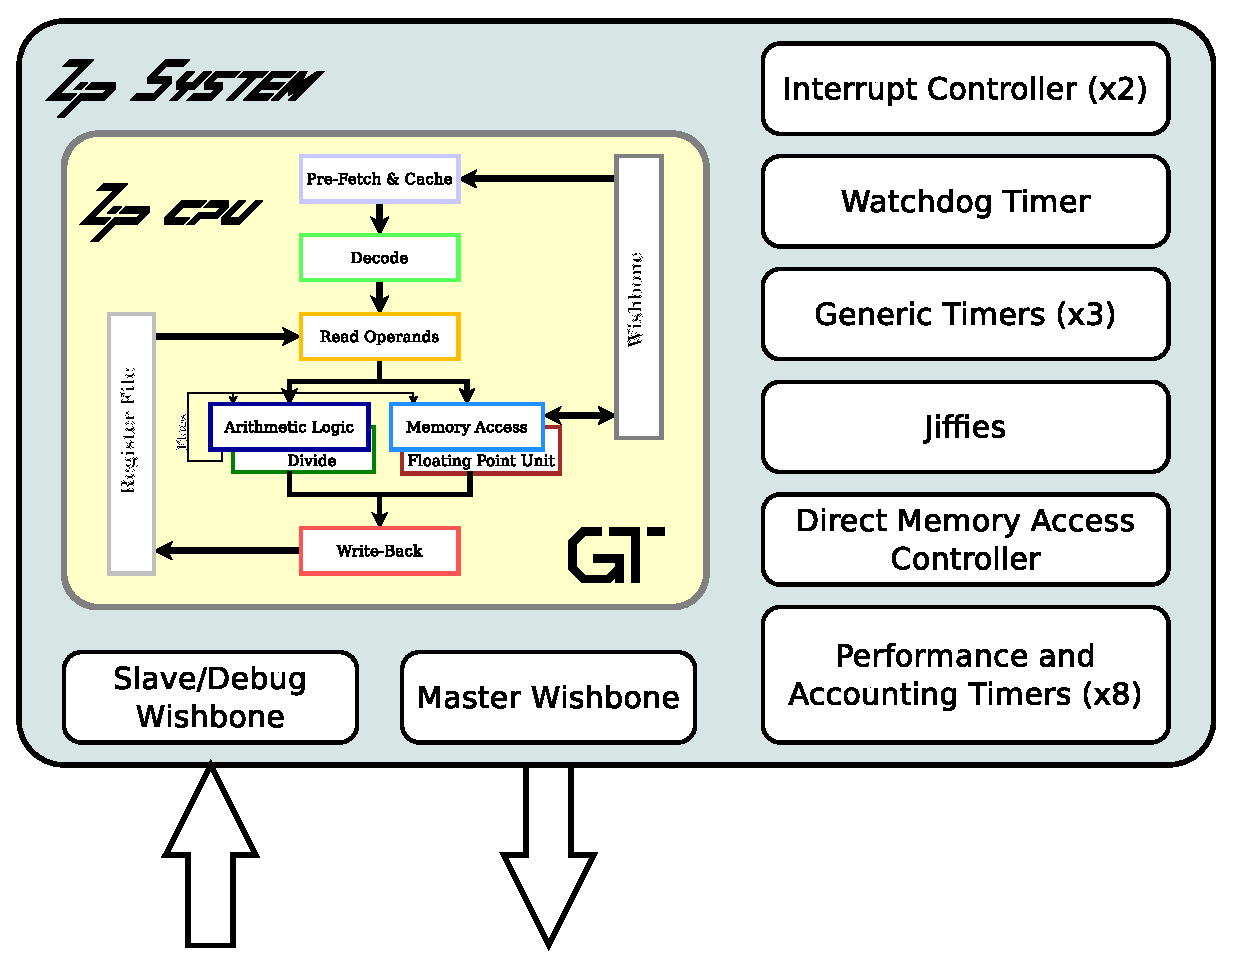
\includegraphics[width=3.5in]{../gfx/system.eps}
\caption{ZipSystem Peripherals}\label{fig:zipsystem}
\end{center}\end{figure}
and described here.  They are designed to make
the ZipCPU more useful in an Embedded Operating System environment.
%% }}}
\section{Document Scope}\label{sec:limits}
%% {{{
The ZipCPU is itself nothing more than a CPU that can be placed within a 
larger design.  It is not a System on a Chip, but it can be used to create
a system on a chip.  As a result, this document will not discuss more than a
small handful of CPU--related peripherals, as the actual peripherals used
within a design will vary from one design to the next.  Further, because
control access will vary from one environment to the next, this document will
not discuss any host control programs, leaving those to be discussed and defined
together with the environments the ZipCPU is placed within.
%% }}}
\appendix{Current Assessment}\label{chap:assessment}
%% {{{
Having now worked with the ZipCPU for several years, it is worth offering an
honest assessment of how well it works and how well it was designed. At the
end of this assessment, I will propose some changes that may take place in a
later version of this ZipCPU to make it better.

%%
%% Applications:
%%	(Designed for) GPS Correlator controller
%%	Video configuration handler
%%		Negotiate video clock rate, resolution, etc.
%%	SONAR data recorder
%%	Embedded Hard Drive test bench controller
%%	SONAR transmit controller
%%	FFT accelerator
%%	(NOR flash bringup)
%%	Simulation:
%%		Clock gate testing
%%		Embedded hard drive test bench controller
%%		Embedded flash test bench controller
%%
%%

\section{The Good}
%% {{{
\begin{itemize}
\item The ZipCPU was designed to be a simple and light weight CPU.  It has
	achieved this end nicely.  The proof of this is the full multitasking
	operating system built for Digilent's CMod S6 board, based around
	a very small Spartan~6/LX4 FPGA. 

	As a result, the ZipCPU also makes a good starting point for anyone
	who wishes to build a general purpose CPU and then to experiment with
	building and adding particular features.  Modifications should be
	simple enough. 

	Indeed, a non--pipelined version of the bare ZipBones (with no
	peripherals) has been built that only uses 1.5k~6--LUTs.  When using
	pipelining, the full cache, and all of the peripherals, the ZipSystem
	can take up to 4.6~k LUTs.  Where it fits in between is a function of
	your needs.

	When using an iCE40 FPGA, the minimal ZipBones wrapper plus the
	ZipCPU will fit nicely within the 2.7k~4-LUTs.

%% Fits its role
\item The ZipCPU was designed to be placed within an FPGA and so to control the
	actions within an FPGA.  It fits this role rather nicely.

	Some capabilities common to more general purpose CPUs, such as a
	floating point capability, vector registers and vector operations have
	been left out in favor of lower logic usage.  However, it was never
	designed to be such a general purpose CPU but rather a system within
	a chip.  

%% Simple instruction set
\item The extremely simplified instruction set of the ZipCPU has proven to be
	a good choice. Indeed, it is good enough that the ZipCPU has not needed
	an instruction set upgrade between version 2.0 and 3.0.  Although this
	instruction set does not have many of the commonly used instructions,
	PUSH, POP, JSR, and RET among them, the simplified instruction set has
	demonstrated an amazing versatility. I will contend therefore and for
	anyone who will listen, that this instruction set offers a full and
	complete capability for whatever a user might wish to do--with the
	only exception being accelerated floating-point or vector operation
	support.

%% Interrupt approach
\item The ZipCPU's approach to interrupts greatly facilitates the development
	of interrupt handlers from within high level languages.

	The approach involves a single interrupt ``vector'' only, and simply
	switches the CPU back to the instruction it left off at.  By using
	this approach, interrupt handlers no longer need careful assembly
	language scripting in order to save their context upon any interrupt.

	At the same time, if most modern systems handle interrupt vectoring in
	software anyway, why maintain complicated hardware support for it?

%% Tool suite
\item A complete tool suite consisting of GCC, binutils, newlib, and FATFS
	support now exists.
\end{itemize}
%% }}}

\section{The Not so Good}
%% {{{
\begin{itemize}
%% 3 Operand instructions
\item Many other instruction sets offer three operand instructions, whereas
	the ZipCPU only offers two operand instructions. This means that it
	may take the ZipCPU more instructions to do many of the same operations.
	The good part of this is that it gives the ZipCPU a greater amount of
	flexibility in its immediate operand mode.

	The impact of this lack of three operand instructions is application
	dependent, but does not appear to be too severe.

%% OOM
\item The ZipCPU doesn't support out of order execution.

	I suppose it could be modified to do so, but then it would no longer
	be the ``simple'' and low LUT count CPU it was designed to be.

%% Context switching
\item Although switching to an interrupt context in the ZipCPU design doesn't
	require a tremendous swapping of registers, in reality it still
	does--since any task swap (such as swapping to a task waiting on an
	interrupt) still requires saving and restoring all 16~user registers.
	That's a lot of memory movement just to service an interrupt.

	This isn't nearly as bad as it sounds, however, since most RISC
	architectures have 32~registers that will need to be swapped upon any
	context swap.

%% 4GB address space
\item The ZipCPU cannot handle addresses larger than 32-bits (4GB).
	This is a fundamental common to all 32-bit architectures, the ZipCPU
	included.  While an MMU might help this problem, user
	tasks would remain limited to 4GB of addressable memory.

	Given that both memory and peripherals must share the same bus, this
	effectively limits the ZipCPU's memory to 2GB.

	While this may limit the ZipCPU's utility as a generic CPU in the
	future, the limitation has yet to impact any of my projects.

%% GDB
\item The ZipCPU doesn't yet have full gdb support.  This may be provided
	in future versions.

%% Memory and DMA
\item When using a DMA to move memory, the only way to tell the CPU that
	memory may have been updated outside of the cache is currently to
	flush the entire cache.  While this isn't ideal, it does work.

%% Loading the ZipCPU
\end{itemize}
%% }}}

\section{The Next Generation}
%% {{{
This section could also be labeled as my ``To do'' list.  It outlines where
you may expect features in the future.  Currently, there are two primary
items on my to do list:
\begin{enumerate}
\item An optional Memory Management Unit

	An MMU is necessary to run Linux.  Linux, however, may easily get in the
	way of the ZipCPU's typically deeply embedded application.  As a
	bare metal (no O/S) CPU, the ZiPCPU does nicely without any MMU.  An
	MMU might first be a challenge to configure, and second it would be
	likely to slow down every memory access by one to two clock cycles.

	So, is an MMU truly necessary?

	Where not having an MMU becomes problematic is when trying to keep
	tasks running on the ZipCPU from overrunning their stack or smashing
	into another tasks memory area.  For this reason alone, an MMU could
	be valuable.

	The first version of an MMU has already been written.  It is 
	available for examination in the ZipCPU repository.  This MMU
	however, did not make it to integration.  The current
	3.0~architecture should make integrating an MMU easier.

\item An integrated floating point unit (FPU)

	Why a small scale CPU needs a hefty floating point unit, I'm not
	certain, but many application contexts require the ability to do
	floating point math.  This need is currently provided via GCC's
	floating point emulation library.  Whether a true floating point
	unit is really necessary is an open question--and one of the reasons
	why it has not (yet) been written.

% \item ROM instruction space

\end{enumerate}
%% }}}
%% }}}
\fi
